% ================================================
% Please HIGHLIGHT the new inputs such like this :
% Text :
%  \hl{comment}
% Aligned Eq. 
% \begin{shaded}
% \end{shaded}
% ================================================

\documentclass[letter,journal]{IEEEtran}

%\usepackage[retainorgcmds]{IEEEtrantools}
%\usepackage{bibentry}  
\usepackage{xcolor,soul,framed} %,caption

\colorlet{shadecolor}{yellow}
% \usepackage{color,soul}
\usepackage[pdftex]{graphicx}
\graphicspath{{../pdf/}{../jpeg/}}
\DeclareGraphicsExtensions{.pdf,.jpeg,.png}

\usepackage[cmex10]{amsmath}
%Mathabx do not work on ScribTex => Removed
%\usepackage{mathabx}
\usepackage{array}
\usepackage{mdwmath}
\usepackage{mdwtab}
\usepackage{eqparbox}
\usepackage{url}

\hyphenation{op-tical net-works semi-conduc-tor}

%\bstctlcite{IEEE:BSTcontrol}

\usepackage{multicol}
\usepackage{multirow}
\usepackage{array}
\usepackage{bm} % bold math
\usepackage{tabularx}
\usepackage[caption=false,font=footnotesize]{subfig}
\usepackage{cite}
\usepackage{hhline}
\usepackage{tikz}

\usepackage{makecell}
\usepackage{caption}
\usepackage{threeparttable}


%=== TITLE & AUTHORS ====================================================================
\begin{document}
\bstctlcite{IEEEexample:BSTcontrol}
    \title{A Real-Time Deep Reinforcement Learning Processor for Mapless Autonomous Navigation with Unified Actor-Critic Network and Inference-on-Request Scheduling}
  \author{Juyoung~Oh,~\IEEEmembership{Graduate Student Member,~IEEE,}
      Jie-Xin~Liu,
      Yi-Chen~Teng,\\
      Hsueh-Cheng~Wang,~\IEEEmembership{Member,~IEEE,}
      and~Dongsuk~Jeon,~\IEEEmembership{Member,~IEEE}% <-this % stops a space

  \thanks{Received 21 Jun 2025; revised 4 Oct 2025; accepted 24 Oct 2025. This work was supported in part by the Institute of Information and Communications Technology Planning and Evaluation (Grant RS-2025-02218733, 50\%) and National Research Foundation of Korea (Grant RS-2025-04162969, 50\%). (Corresponding author: Dongsuk Jeon.)}

  \thanks{Juyoung Oh and Dongsuk Jeon are with the Department of Intelligence and Information, the Research Institute for Convergence Science, and the Inter-University Semiconductor Research Center, Seoul National University, Seoul 08826, South Korea (e-mail: djeon1@snu.ac.kr).

  Jie-Xin Liu, Yi-Chen Teng, and Hsueh-Cheng Wang are with the Institute of Electrical and Control Engineering, National Yang Ming Chiao Tung University, Hsinchu 30010, Taiwan.
  }% <-this % stops a space
  }

% The paper headers
\markboth{IEEE JOURNAL OF SOLID-STATE CIRCUITS, VOL. xx, NO. x, MARCH 2026
}{Oh \MakeLowercase{\textit{et al.}}: Real-Time Reinforcement Processor}
% ====================================================================
\maketitle



% === ABSTRACT ====================================================================

\begin{abstract}
This paper presents a real-time deep reinforcement learning processor for mapless autonomous navigation targeting resource- and energy-constrained mobile robots. The unified actor-critic network architecture combined with feature map caching enables parameter sharing and eliminates redundant computations. This approach reduces the total parameter count, external memory access, and overall operations by 95.6\%, 84.1\%, and 85.4\%, respectively, without compromising learning performance. The processor further incorporates an inference-on-request scheduling scheme to achieve concurrent training and inference, thereby ensuring low inference latency and maintaining high processing element utilization of 71.0\% including external I/O overhead. A column-wise zero-skipping categorical projection accelerates distributional reinforcement learning by processing only non-zero entries in the sparse $\Delta h$ matrix, achieving a 99\% reduction in projection operations. Fabricated in a 28-nm CMOS process, the chip consumes 2.68 mW with a 10-MHz clock frequency, meeting the real-time latency requirements. The processor was verified on a real robot, demonstrating robust autonomous navigation ability in unseen environments. To the best of our knowledge, this is the first design to support distributional reinforcement learning, and experimental results with a real robot confirm both the effectiveness and practical viability of the design.
\end{abstract}
 

% === KEYWORDS ====================================================================
% =================================================================================
\begin{IEEEkeywords}
Deep reinforcement learning, neural network accelerator, autonomous navigation, task scheduling, adaptive dataflow.
\end{IEEEkeywords}

% For peer review papers, you can put extra information on the cover
% page as needed:
% \ifCLASSOPTIONpeerreview
% \begin{center} \bfseries EDICS Category: 3-BBND \end{center}
% \fi
%
% For peerreview papers, this IEEEtran command inserts a page break and
% creates the second title. It will be ignored for other modes.
\IEEEpeerreviewmaketitle
% ====================================================================
% ====================================================================
% ====================================================================


% === I. INTRODUCTION =============================================================
% =================================================================================
\section{Introduction}

\IEEEPARstart{M}{apless} autonomous navigation, which refers to navigating without pre-existing map information, has emerged as a critical requirement for mobile robots deployed in unknown or dynamic environments \cite{iros17, iros23, icra21}. As illustrated in Fig. \ref{fig:mapless_navigation}, mapless autonmous navigation leverages only on-board sensor observations to accomplish the navigation task, allowing the robot to flexibly adapt to unseen and changing environments. Traditional approaches relying on global maps and precise localization are often impractical due to the frequent unavailability or unreliability of environmental data, as well as the high cost of building and maintaining maps in real-world settings \cite{iros17}. Recent advances in deep reinforcement learning (DRL) have enabled the direct learning of navigation policies from sensor observations and goal coordinates, removing the need for manual feature design and expert demonstrations. DRL-based mapless navigation has demonstrated robust performance and generalization for a variety of robotic platforms including ground, aerial, and underwater robots by utilizing sparse range measurements and relative localization as input features \cite{iros17, iros23}.

\begin{figure}[!t]
   \begin{center}
  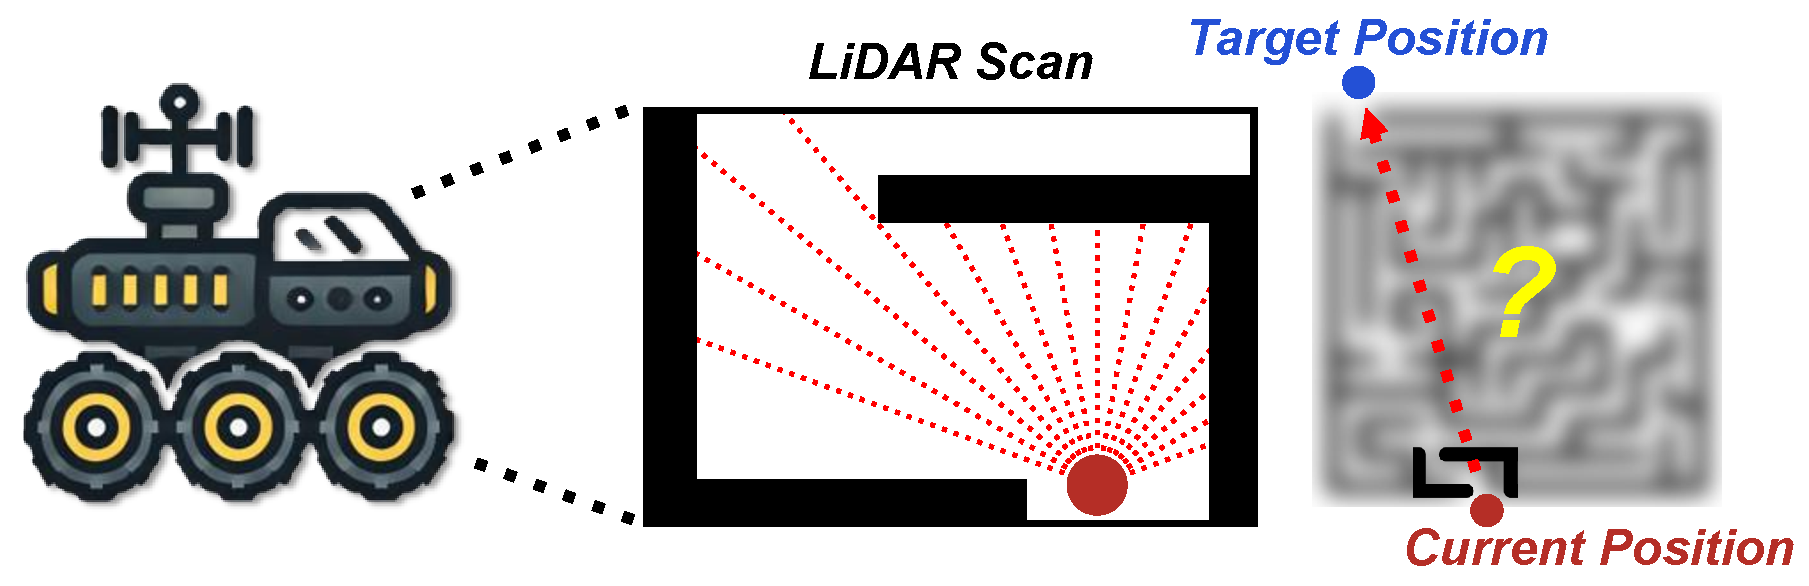
\includegraphics[width=3.5in]{Figures/Fig_mapless_navigation.pdf}\\
  \caption{Example of mapless autonomous navigation.}\label{fig:mapless_navigation}
   \end{center}
   \vspace{-0.5cm}
\end{figure}


While traditional DRL algorithms, such as Twin Delayed Deep Deterministic Policy Gradient (TD3) \cite{TD3}, represent expected rewards as scalar Q values, this approach does not sufficiently capture the uncertainty inherent in navigation tasks under ambiguous or dynamic conditions \cite{ur23, AAAI19}. In contrast, distributional reinforcement learning (DistRL) methods, such as C51 \cite{C51} and Distributed Distributional Deep Deterministic Policy Gradient (D4PG) \cite{d4pg}, model Q values as distributions, providing improved uncertainty estimation and greater robustness in policy execution. Recent studies have shown that DistRL approaches offer superior reliability and adaptability in mapless navigation tasks, particularly when facing unstructured or unpredictable environments \cite{ur23, nctu_fr, NCTU}.

Recent real-world navigation studies increasingly adopt a two-stage training scheme where policies are pre-trained offline using a simulator and then fine-tuned online in the deployment environment \cite{lifelong, selfi, fastrlap}. This approach is effective since pre-training provides general navigation priors, and online fine-tuning equips the robot with environment-specific behaviors that adapt the policy to the target setting. Moreover, building a high-fidelity simulation environment for every target environment is nontrivial, as setting up the simulator is time-consuming and modeling the 3D scene itself demands substantial effort \cite{iros_interview}. Consequently, starting from well-trained policy and fine-tuning it in the target environment is often the efficient way to the deployment.

Despite these algorithmic advances, deploying DRL for real-time, on-device navigation presents significant hardware and system-level challenges. State-of-the-art algorithms, including TD3 \cite{TD3} and D4PG \cite{d4pg}, require multiple network evaluations per control step, which substantially increases external memory access (EMA) and computational demand, which are major bottlenecks in embedded platforms subject to stringent power and latency constraints. DistRL further amplifies these resource requirements due to the additional cost of probability redistribution.

To address these challenges, a number of energy-efficient DRL accelerators have been proposed. The authors in \cite{ISSCC19} presented a DRL accelerator with a transposable PE array and experience compression, which reduced memory bandwidth and power consumption through dynamic data reuse. OmniDRL \cite{VLSI21} introduced dual-mode weight compression, an on-chip sparse weight transposer, and an exponent encoding scheme to enable flexible dataflow. The design in \cite{TCASII24} employs delta-based weight sharing and block-mantissa reconfigurable PE arrays, which further reduced EMA and supported flexible precision for various neural network workloads. The authors in \cite{CICC25} presented a processor capable of full speculation exploitation and parallel inference-training processing, achieving high utilization and efficiency by leveraging dynamic data sparsity, binary direct feedback alignment, and sparse data encoding.

While these prior works have made significant progress in improving hardware efficiency and throughput for RL workloads, they have mainly targeted DRL algorithms based on scalar Q-values, as well as lacked the flexibility and responsiveness required for dynamic workload scheduling and strict real-time control in practical robotic applications.

In this work, we present a real-time DRL processor for mapless autonomous navigation that achieves both high energy efficiency and robust adaptation to unseen environments. The key contributions of this work are as follows:
 \begin{enumerate}
    \item A unified actor-critic network architecture with feature map caching, which substantially reduces total parameters, EMA, and computational costs
    \item An Inference-on-Request (IoR) scheduling scheme for low-latency inference and high processor utilization
    \item Adaptive dataflow mapping to maximize PE utilization across diverse workload patterns
    \item A column-wise zero-skipping categorical projection scheme to efficiently support DistRL
\end{enumerate}

The remainder of this article provides a detailed description of our previously published conference paper \cite{RL_CICC}, along with additional elaboration and new experimental results. More specifically, this paper provides a detailed architectural description and processing flow of the unified actor–critic network. It also presents ablation studies that validate the effectiveness of parameter sharing and demonstrate applicability to other DRL algorithms. In addition, it elaborates more on critical hardware components, including the on-chip memory structure, the end-to-end execution flow, and the column-wise zero-skipping categorical projection, with substantially expanded explanations. Finally, experimental results from diverse simulation environments are included to highlight the generality and efficiency of the design. In Section \ref{sec:network}, we introduce the proposed unified actor-critic network architecture and feature map caching technique with ablation study and experiments. Section \ref{sec:processor} presents hardware optimization techniques including IoR scheduling, adaptive dataflow mapping, and column-wise zero-skipping categorical projection. Section \ref{sec:results} shows chip measurement results and experimental evaluations, followed by conclusions in Section \ref{sec:conclusion}.

\section{Unified Actor-Critic Network} \label{sec:network}
\subsection{Network Architecture}

\begin{figure}[!t]
\centering

\subfloat[]{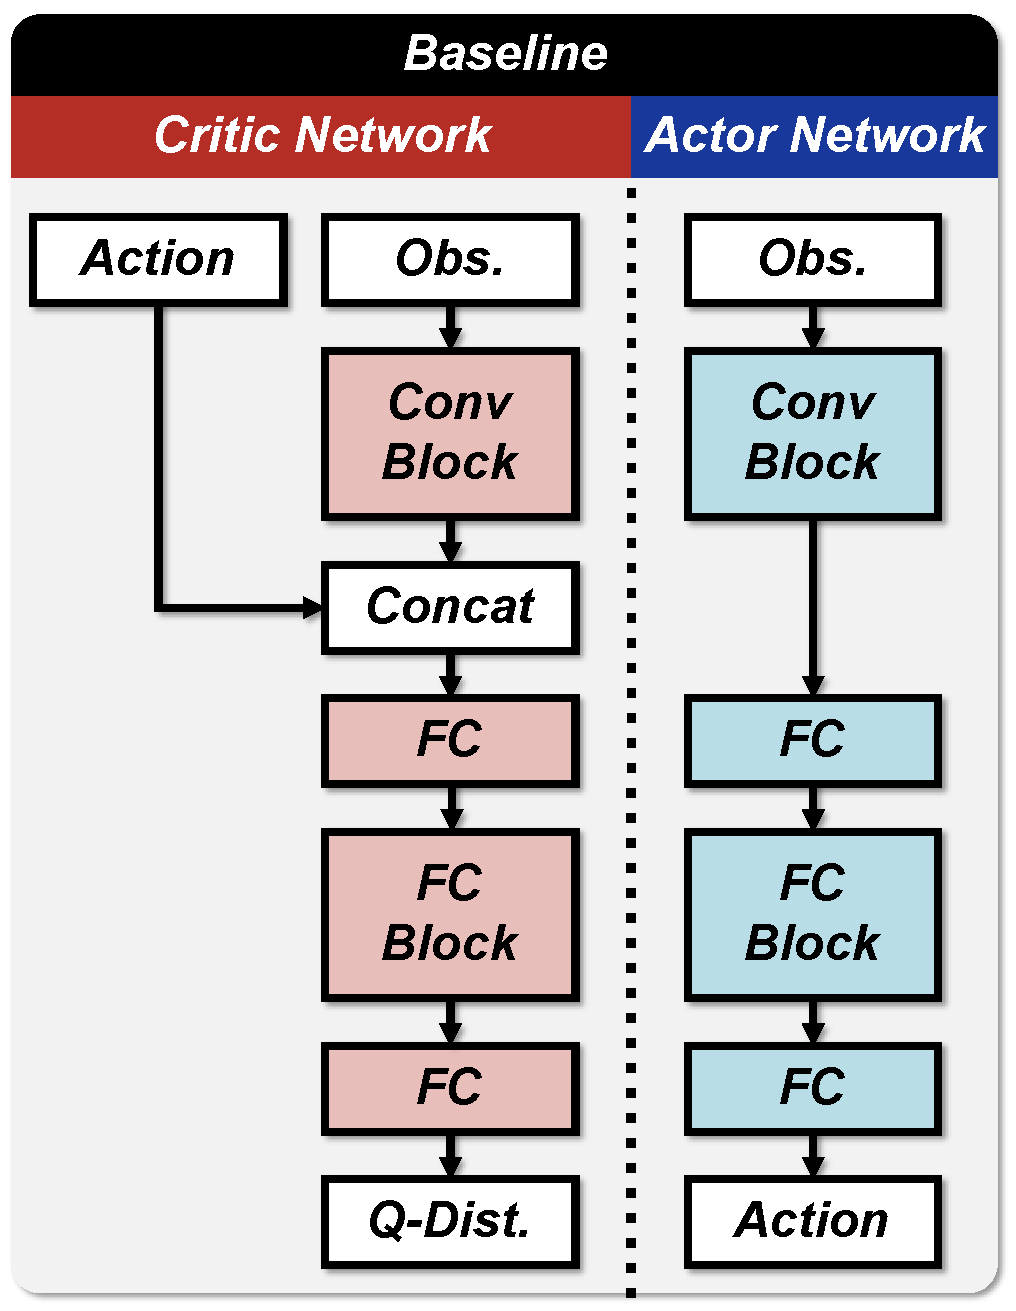
\includegraphics[height=6cm]{Figures/Fig_baseline_network_v3.pdf}\label{fig:baseline_network}}
\hspace{1mm}
\subfloat[]{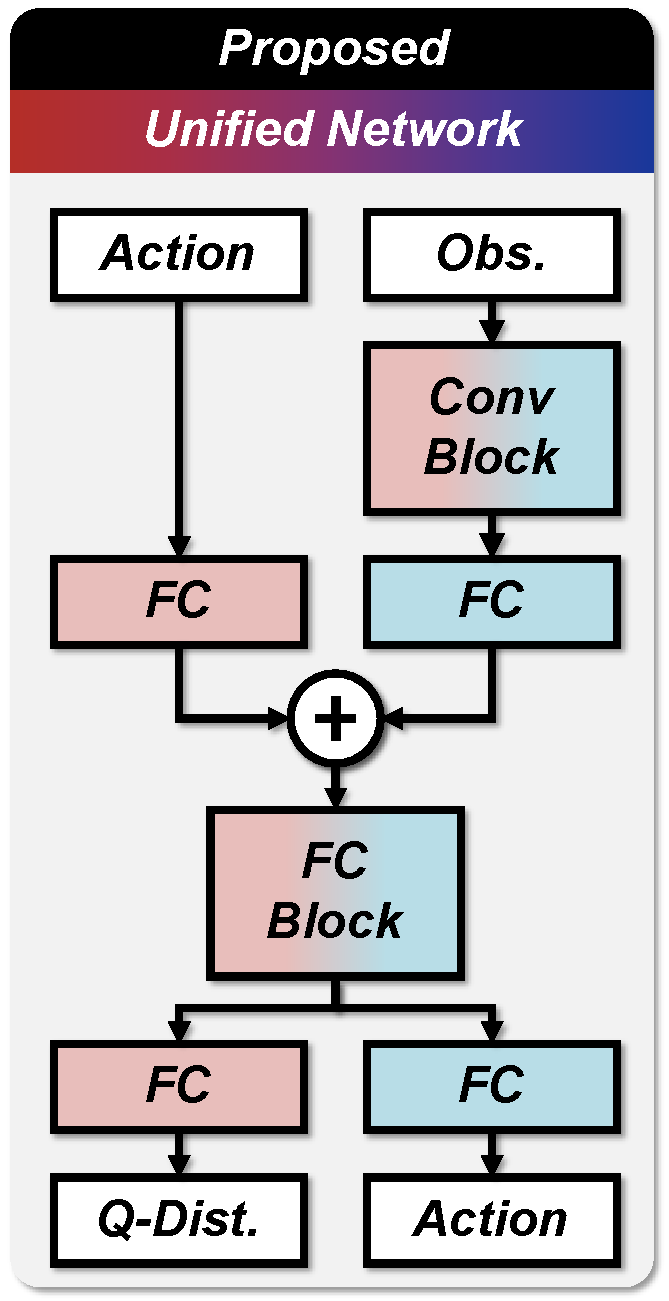
\includegraphics[height=6cm]{Figures/Fig_unified_network_v3.pdf}\label{fig:unified_network}}

\caption{(a) Baseline network architecture and (b) proposed unified actor-critic network.}\label{fig:networks}
\vspace{-0.5cm}
\end{figure}



D4PG \cite{d4pg} adopts an actor-critic network architecture, in which two separate types of neural networks are employed: an actor network, which generates an action given the current observation, and a critic network, which evaluates the quality of that action in a specific state. Fig. \ref{fig:networks}\subref{fig:baseline_network} shows the baseline architecture for D4PG used in prior work on mapless autonomous navigation \cite{NCTU}. The observation input to the network consists of three components: 2D laser-scan range data converted from 3D LiDAR point clouds, semantic segmentation labels, and the relative position of the robot with respect to its goal. They are first processed by a shared convolutional (Conv) block that extracts meaningful features from the input. The actor network generates actions from extracted features using fully connected (FC) layers. On the other hand, the critic network evaluates the quality of a given action in a specific state by taking both the extracted features (observation) and the action as inputs. These inputs are concatenated and processed through additional FC layers to produce a value function representing the evaluation of the state-action pair. Value functions are fundamental to reinforcement learning, as they provide a quantitative measure for evaluating states and actions. The state-value function (V-function) estimates the expected cumulative reward from a given state, while the action-value function (Q-function) estimates the expected return of taking a specific action in a specific state \cite{rl_intro}. D4PG, like many actor-critic algorithms, relies on the Q-function, requiring the critic to process both observation and action as inputs.

Given the architectural similarity between the actor and critic networks, we propose unified network structure that shares the majority of convolutional and FC layers, as shown in Fig. \ref{fig:networks}\subref{fig:unified_network}. To address functional differences, only a few FC layers remain separate, allowing each branch to capture task-specific features while benefiting from a largely shared backbone.

A key challenge in unifying the actor and critic architectures using Q-functions arises from their different input requirements: the critic network must process both the observation and the action, while the actor only requires the observation. To resolve this, the unified network employs a shared first FC layer that processes only observation-derived features, consistent with the actor pathway. For the critic, a lightweight additional FC layer processes the action input independently. The outputs of these two branches are then combined element-wise, allowing the remaining FC layers to be fully shared.

Beyond this point, all subsequent FC layers, represented as \textit{FC block} in the figure, are shared between the actor and critic, minimizing parameter redundancy. The final FC layer, however, is kept separate for each branch to accommodate the distinct output requirements: the actor produces a continuous action, while the critic outputs a Q-value. In Fig. \ref{fig:networks}\subref{fig:unified_network}, the layers depicted with a color gradient indicate the portions of the network shared between the actor and critic in the unified architecture. Red-colored layers are exclusive to the critic network, and blue-colored layers are exclusive to the actor network. This approach enables efficient parameter sharing and results in a compact model, while still allowing each branch to specialize as necessary for its respective task.

\begin{figure}[!t]
   \begin{center}
  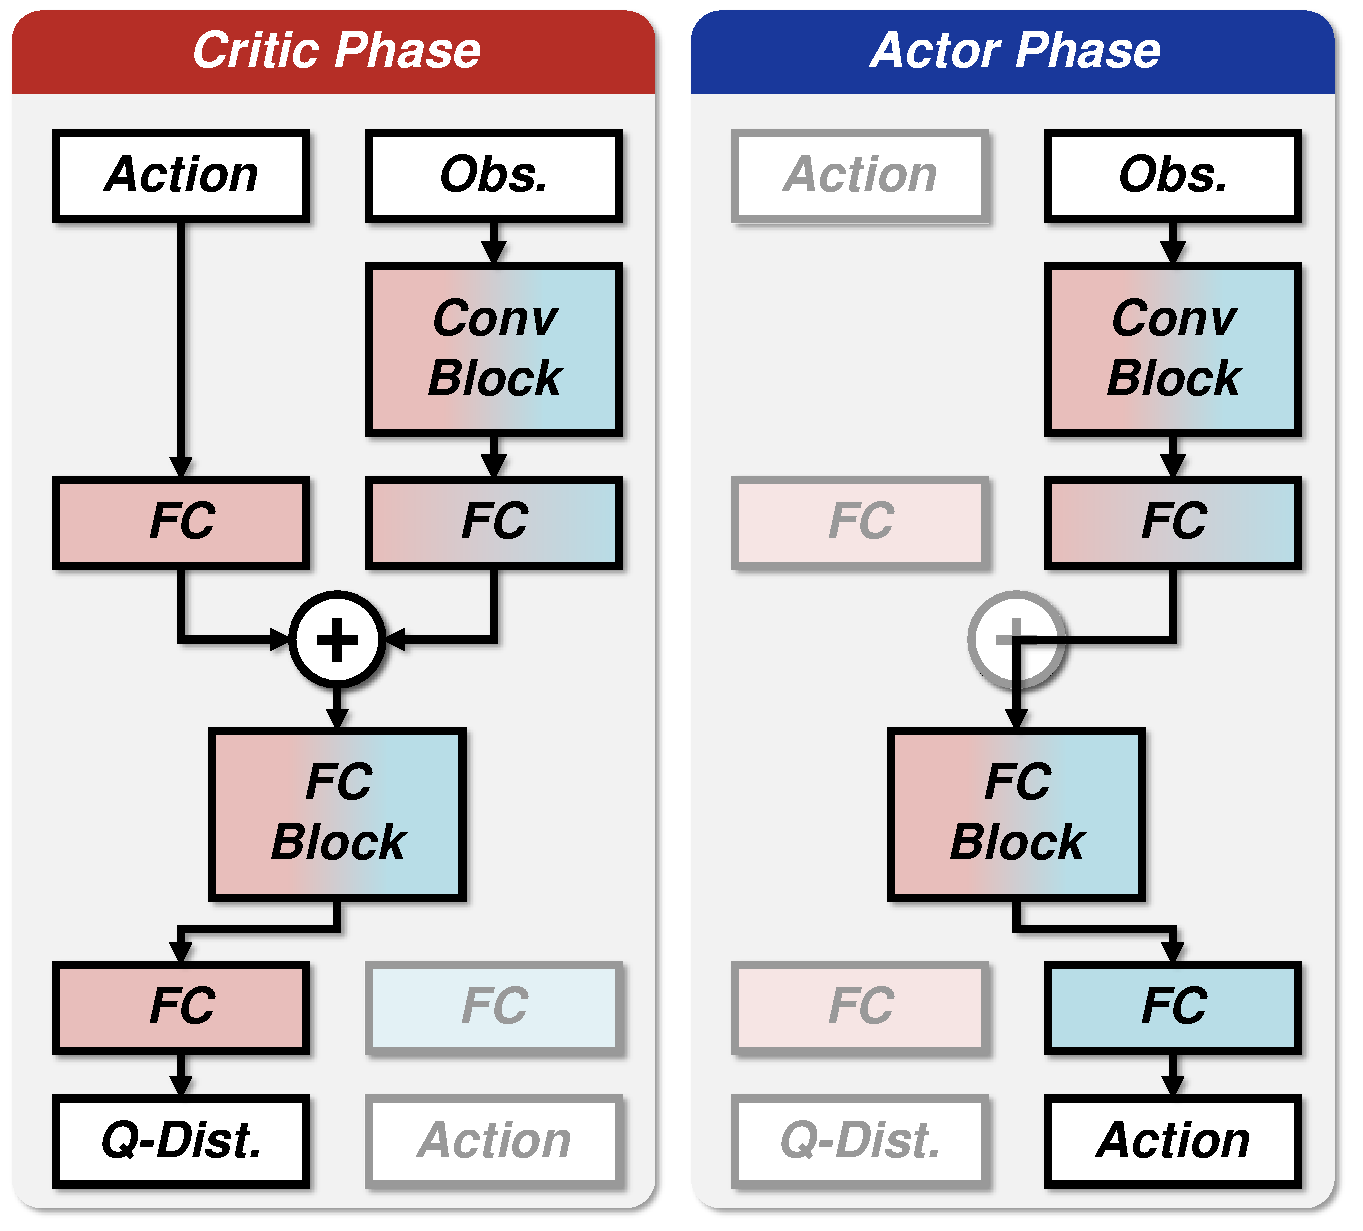
\includegraphics[width=0.8\linewidth]{Figures/Fig_network_flow.pdf}\\
  \caption{Processing flow of unified network architecture.}\label{fig:Network_flow}
   \end{center}
   \vspace{-0.5cm}
\end{figure}

\begin{figure}[!t]
   \begin{center}
  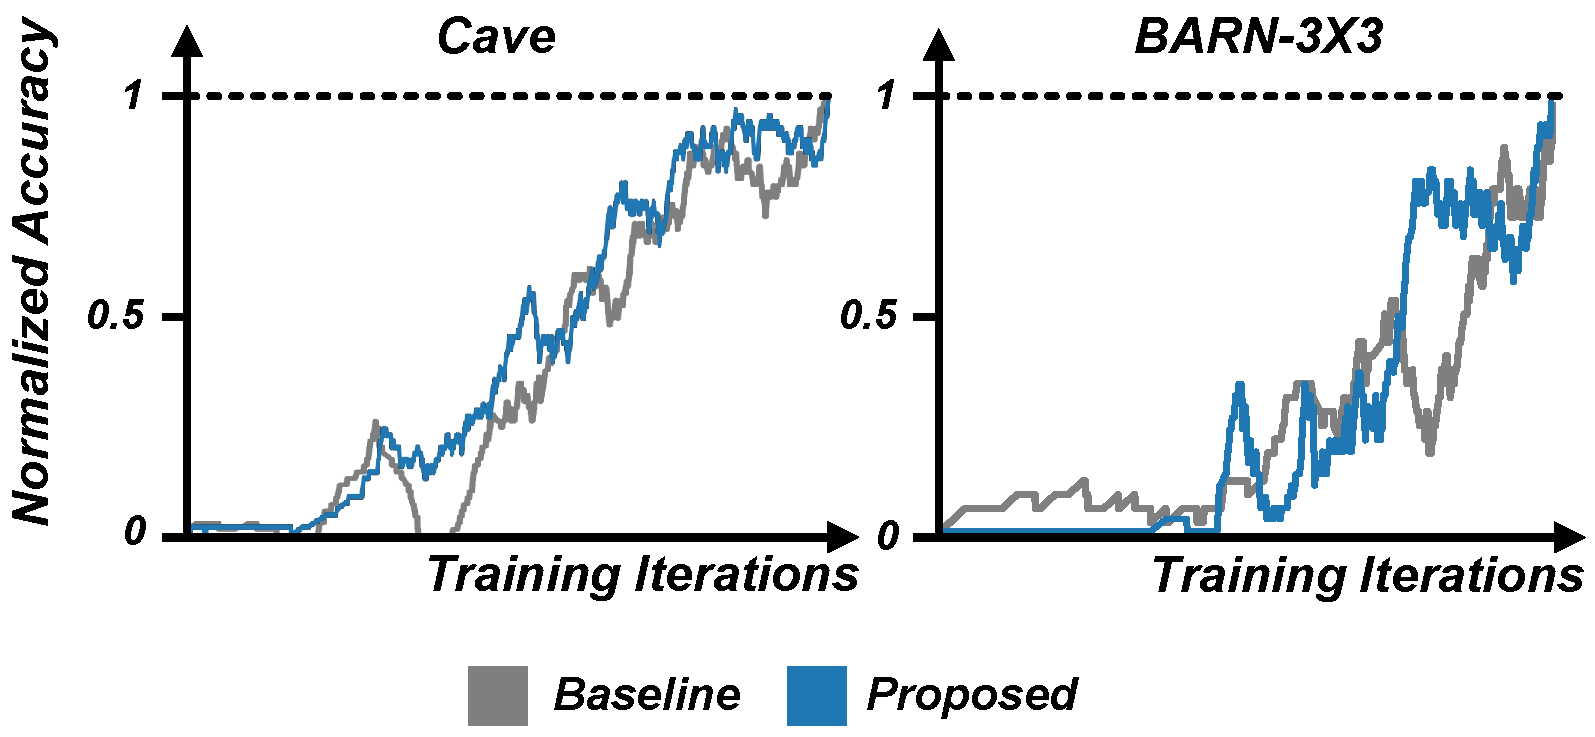
\includegraphics[width=0.9\linewidth]{Figures/Fig_unified_learning_curve_v2.pdf}\\
  \caption{Comparison of baseline network and proposed unified actor-critic network architecture.}\label{fig:Learning_curve}
   \end{center}
   \vspace{-0.5cm}
\end{figure}

Fig. \ref{fig:Network_flow} illustrates the dataflow of the unified actor-critic network architecture, detailing the layers utilized in the critic and actor phases. In the critic phase, the input observation passes through a shared convolutional block and the first FC layer, while the input action is processed by a lightweight, action-specific FC layer. The outputs of these two branches are then combined via element-wise addition and subsequently processed by a shared FC block and a critic-specific last FC layer to produce the Q-value. On the other hand, during the actor phase, only the observation is provided as input. It is propagated through the shared convolutional block, all subsequent FC layers, and the actor-specific last FC layer to generate the action output. Notably, the path related to the action input is omitted in the actor phase, and element-wise addition is not performed.

In the proposed architecture, element-wise addition is performed during the critic phase, whereas the actor phase does not include such operations. This difference in processing may cause a mismatch in the magnitudes of the feature maps generated in each phase. To ensure consistency, the critic phase divides the sum by two, thereby aligning the mean of the feature magnitudes between two phases.

The proposed network architecture was evaluated in multiple simulation environments, including Cave \cite{env_cave} and BARN-3X3 \cite{NCTU}. For comparing algorithm performance, the most critical metric is the number of training iterations required to reach the predefined accuracy threshold. Fig. \ref{fig:Learning_curve} shows that both the baseline and the proposed architecture require nearly the same number of training iterations to achieve the target accuracy, indicating that the proposed optimizations do not compromise learning performance.



\subsection{Feature Map Caching}



\begin{figure}[!t]
\centering

\subfloat[]{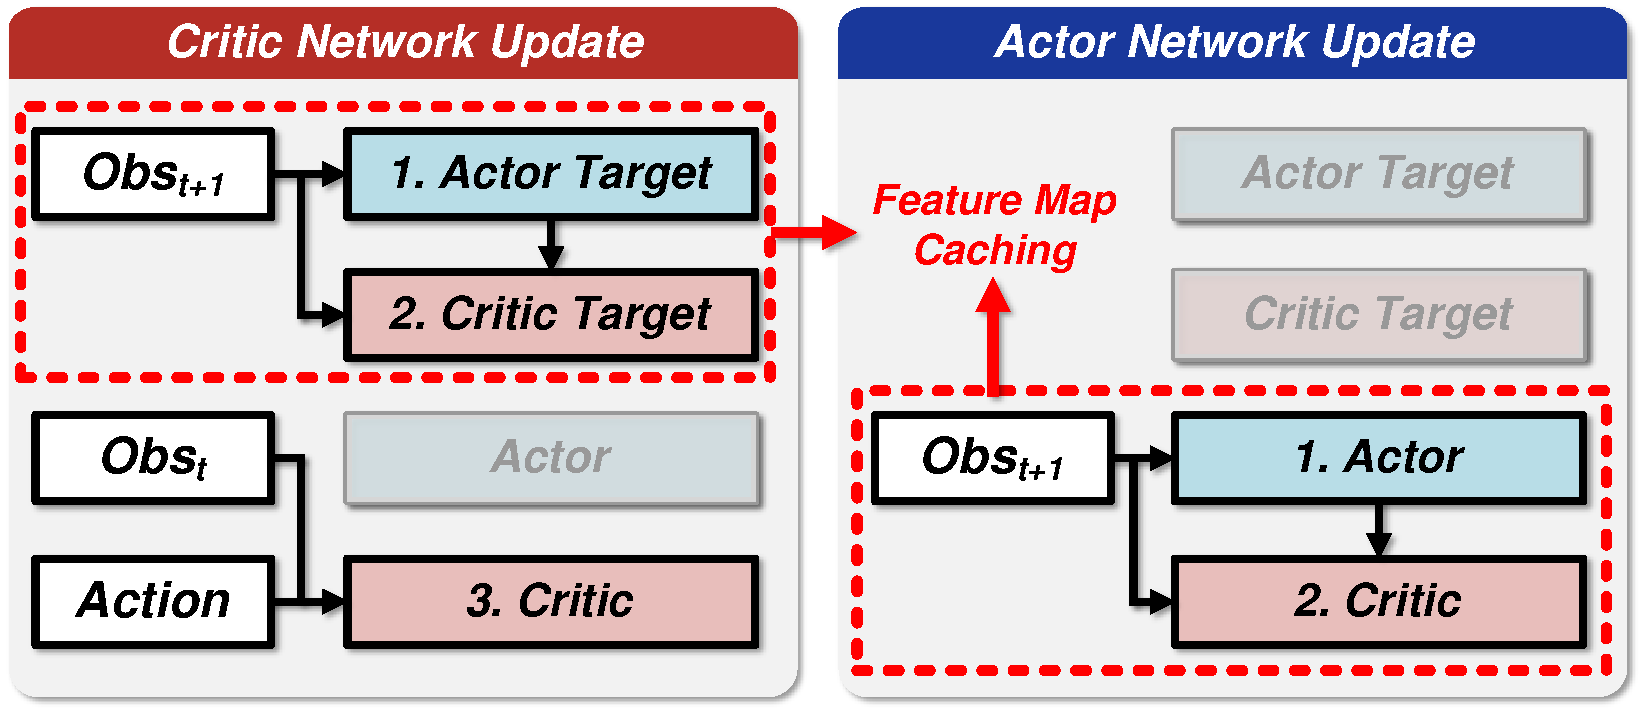
\includegraphics[width=.9\linewidth]{Figures/Fig_training_procedure.pdf}\label{fig:training_procedure}}

\subfloat[]{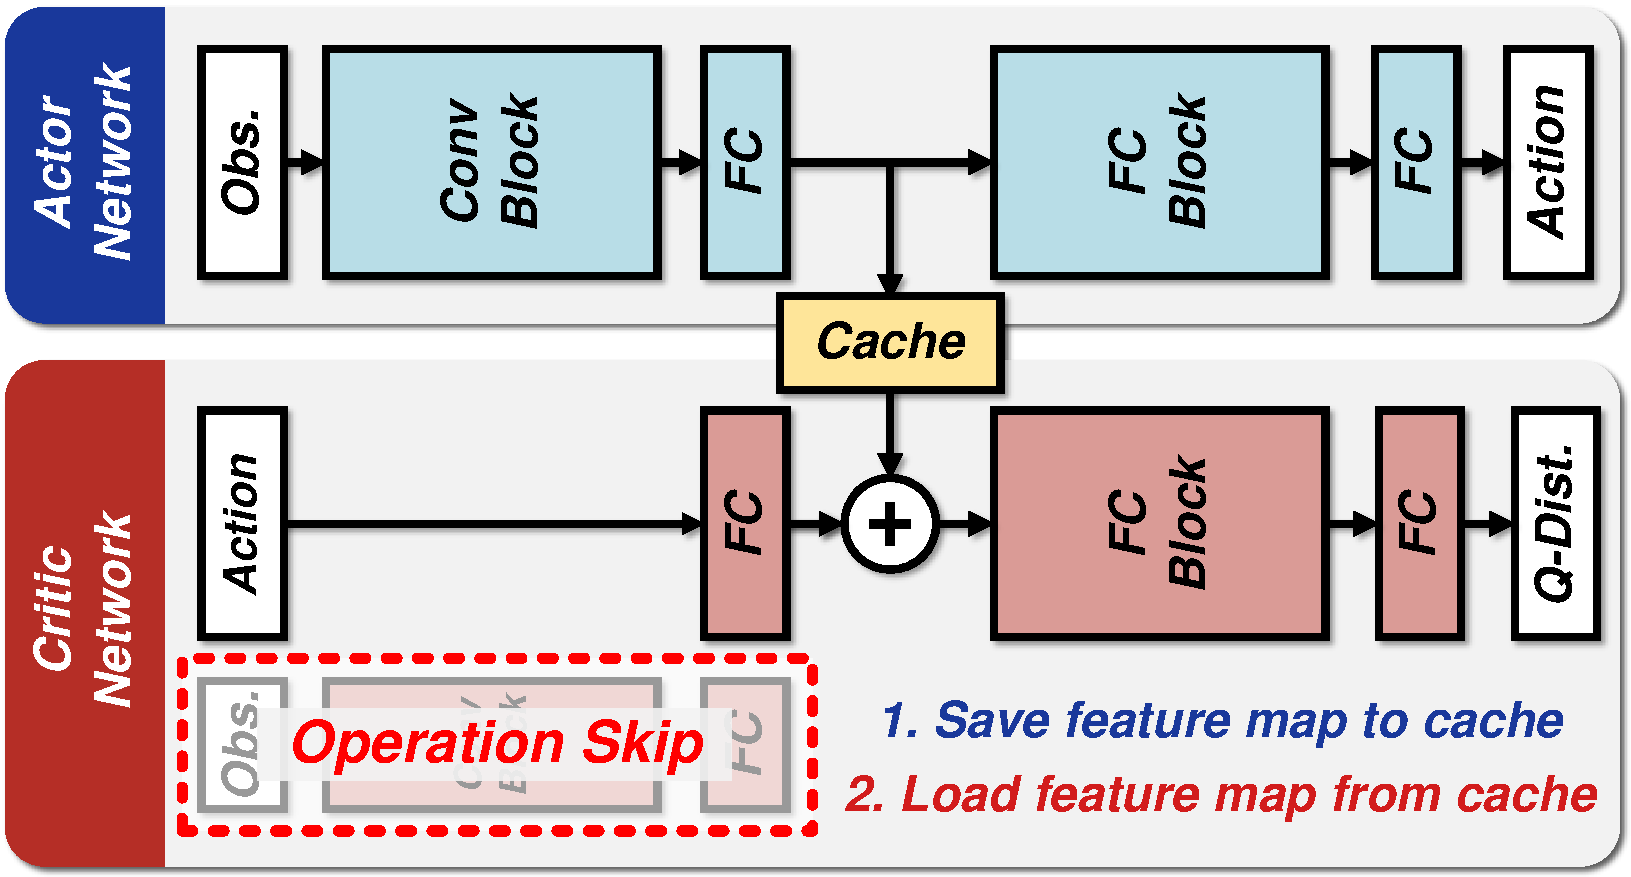
\includegraphics[width=.9\linewidth]{Figures/Fig_feature_map_caching.pdf}\label{fig:feature_map_caching}}

\caption{(a) Training procedure and (b) feature map caching technique.}\label{fig:feature_map_caching_whole}
\vspace{-0.2cm}
\end{figure}

Fig. \ref{fig:feature_map_caching_whole}\subref{fig:training_procedure} illustrates the training procedure of the D4PG algorithm. In the unified network, we maintain target networks for both actor and critic; the main and target networks are architecturally identical, where the target networks for actor and critic share the parameters as well. Both the actor and critic networks are sequentially updated based on the same input observation once in each iteration; the actor network generates an action from the input observation, and both the generated action and the observation are subsequently processed by the critic network. When employing the unified network architecture, the parameters of the shared convolutional block and the first FC layer are identical, resulting in identical output feature maps for the same input observation.



To avoid redundant computation of the identical feature map, we propose a feature map caching technique. As depicted in Fig. \ref{fig:feature_map_caching_whole}\subref{fig:feature_map_caching}, the output of the first FC layer is temporarily stored during the actor phase and later reused in the critic phase. In the critic phase, the cached feature map is loaded and combined with the output feature map from the action-specific FC layer. This approach enables bypassing the redundant convolutional block and the first FC layer computations for the input observation during the critic phase.

\begin{figure}[!t]
   \begin{center}
   % \captionsetup{skip=-5pt}
  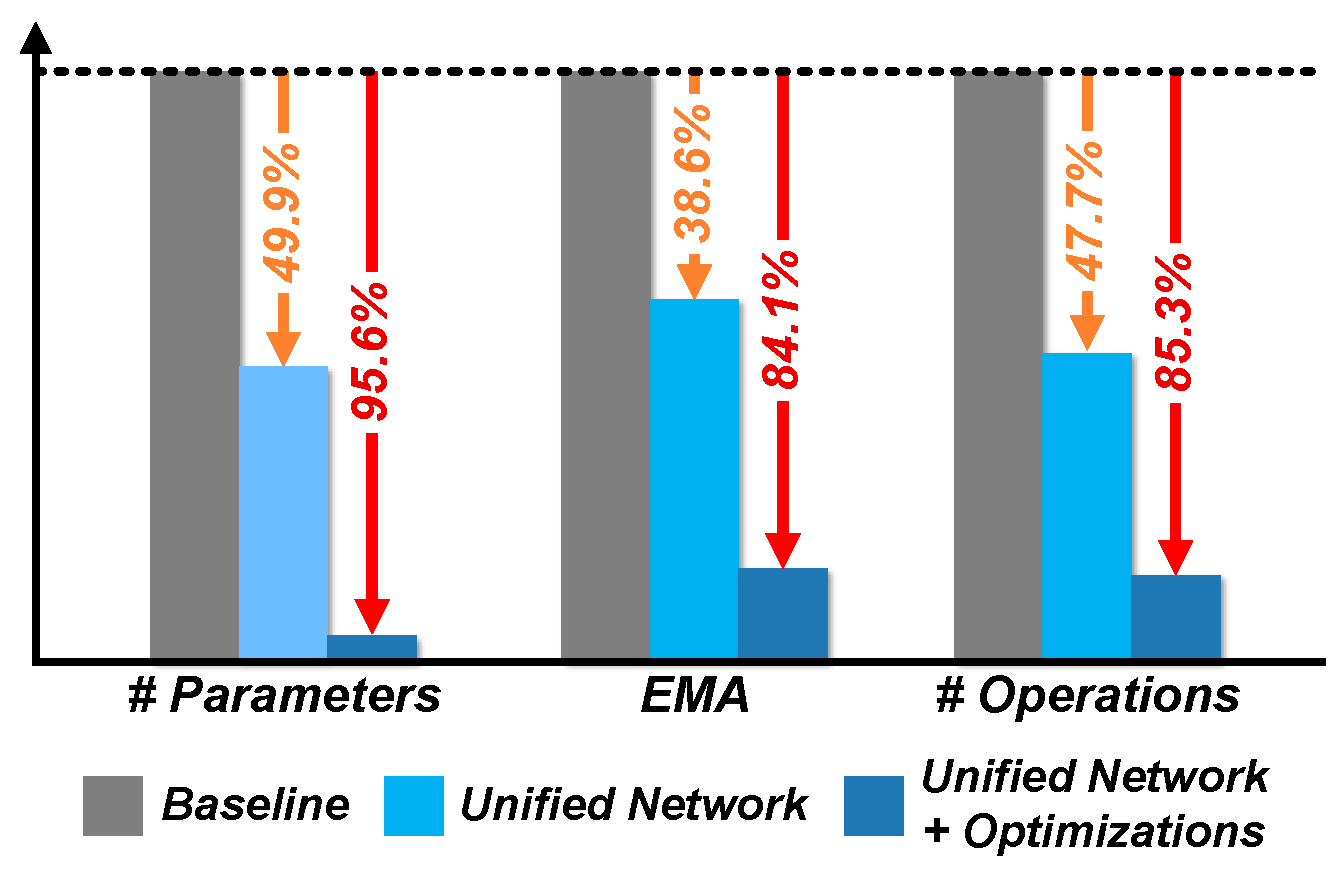
\includegraphics[width=0.8\linewidth]{Figures/Fig_unified_reduction_rev1_v2_cropped.pdf}\\
  \caption{Reductions in parameter, EMA, and operations.}\label{fig:redunction_comparison}
  
   \end{center}
   \vspace{-0.5cm}
\end{figure}

\begin{table}[t]
    \centering
    \caption{Detailed Configurations of Proposed Network}\label{tab:arch_details}
    \vspace{0.1cm}
    
    % 표의 행 높이를 1.5배로 늘립니다.
    \renewcommand{\arraystretch}{1.5} 
    
    \begin{tabular}{|c|c|c|c|}
        \hline
        \textbf{Layer}      & \textbf{\makecell{Input Shape \\ (Cin, Hin) \\ or (Hin)}} & \textbf{\makecell{Filter Size \\ (Cin, Cout, k) \\ or (Hin, Hout)}} & \textbf{\makecell{Activation \\ Function}} \\[8pt]
        \hline
        Conv1               & (4, 482)             & (4, 16, 3)           & ReLU                             \\
        \hline
        Conv2               & (16, 482)            & (16, 16, 3)          & ReLU                         \\
        \hline
        Conv3               & (16, 482)            & (16, 4, 1)           & ReLU                             \\
        \hline
        Conv4               & (4, 482)             & (4, 1, 1)            & ReLU                             \\
        \hline
        FC1\_Shared         & 512               & (512, 512)           & ELU                             \\
        \hline
        FC1\_Critic         & 3                 & (3, 512)             & ELU                          \\
        \hline
        FC2                 & 512               & (512, 512)           & ELU                          \\
        \hline
        FC3                 & 512               & (512, 256)           & ELU                         \\
        \hline
        FC4                 & 256               & (256, 256)           & ELU                          \\
        \hline
        FC5\_Actor          & 256               & (256, 3)             & Tanh                          \\
        \hline
        FC5\_Critic         & 256               & (256, 51)            & -                             \\
        \hline
    \end{tabular}
    \vspace{-0.5cm}
\end{table}

% Fig. \ref{fig:unified_reduction} displays the reductions in total parameter count, EMA, and operation count achieved by the proposed unified network architecture and feature map caching technique. By sharing the majority of layers between the actor and critic networks, the unified network architecture reduces the total parameter count by 95.6\%. While network sharing alone does not decrease EMA or overall computation, applying the feature map caching technique yields substantial reductions; EMA and operation count are decreased by 84.5\% and 85.4\%, respectively. Since the cached feature map is too large to be stored on-chip, it is temporarily saved in off-chip memory, incurring a minor caching overhead that increases the total EMA by 0.4\%. Nevertheless, even with this overhead, the total EMA is finally reduced by 84.1\% compared to the baseline.

Fig. \ref{fig:redunction_comparison} displays the reductions in total parameter count, EMA, and operation count achieved by the proposed unified network architecture and feature map caching technique. By sharing the majority of layers between the actor and critic networks, the unified network architecture reduces the total parameter count by 49.9\%. While network sharing alone does not decrease EMA or overall computation, applying the feature map caching technique yields substantial reductions; EMA and operation count are decreased by 38.6\% and 47.7\%, respectively.

For further optimization of the network, we halved the first two convolution layers' (Conv1 and Conv2) filter channels and introduced two point-wise convolution layers to the baseline network in \cite{NCTU} to reduce the input dimension of the first FC layer (FC1\_Shared). Overall, the total parameter, EMA, and operation count are decreased by 95.6\%, 84.1\% and 85.3\%, respectively.

Table \ref{tab:arch_details} summarizes the details of the proposed network architecture. For the first FC layer (FC1\_Shared), the Conv4 layer output feature map with dimension of 482 is concatenated with the goal-position vector with dimension of 30 to form a 512-dimension input feature map. The network does not employ any normalization layers.

Since the cached feature map is too large to be stored on-chip, it is temporarily saved in off-chip memory, incurring a minor caching overhead that increases the total EMA by 0.4\%. Nevertheless, even with this overhead, the total EMA is finally reduced by 84.1\% compared to the baseline.




\subsection{Ablation Study}

To determine the optimal extent of layer sharing between the actor and critic networks in the proposed unified network architecture, an ablation study was conducted. The experiments considered the following configurations:
 \begin{enumerate}
    \item \textbf{Baseline}: No layer sharing; the actor and critic networks are implemented independently.
    \item \textbf{Sharing Conv only}: Only the convolutional block is shared.
    \item \textbf{Sharing Conv + FC Layer}: The convolutional block and the subsequent first FC layer are shared.
    \item \textbf{Sharing Conv + FC Layer + FC Block}: The convolutional block, first FC layer, and FC block are shared.
\end{enumerate}

The results are summarized in Table \ref{tab:comp}, which reports the number of training iterations required for convergence, total parameter count, EMA, and operation count for each configuration. It is apparent that sharing more layers results in larger reductions in parameter count, EMA, and computation. However, it is interesting to see that the 2nd and 3rd configurations require more training iterations for convergence, despite sharing fewer layers. For a more detailed analysis, the learning curves and the gradient magnitude similarity (GMS), as defined in \cite{GMS}, for each configuration are obtained and displayed in Fig. \ref{fig:ablation_study}. GMS, given by

\begin{table}[t]
    \centering
    \caption{Ablation study results}
    \label{tab:comp}
    \vspace{0.1cm}
    \begin{tabular}{|c|c|c|c|c|}
        \hline
        \textbf{Sharing}             & \textbf{Iterations}   & \textbf{Params}   & \textbf{EMA}     & \textbf{OPs}     \\
        \hline
        Baseline (No sharing)          & 100\%   & 100\%    & 100\%   & 100\%   \\
        \hline Conv only  & 245.61\%& 99.13\%  & 56.87\% & 78.99\% \\
        \hline Conv + FC Layer  & 169.73\%& 81.32\%  & 55.06\% & 68.48\% \\
        \hline \makecell{Conv + FC Layer \\ + FC Block}      & 81.34\% & 50.14\%  & 55.06\% & 50.08\% \\
        \hline
    \end{tabular}
    \vspace{-0.2cm}
\end{table}

\begin{figure}[!t]
   \begin{center}
  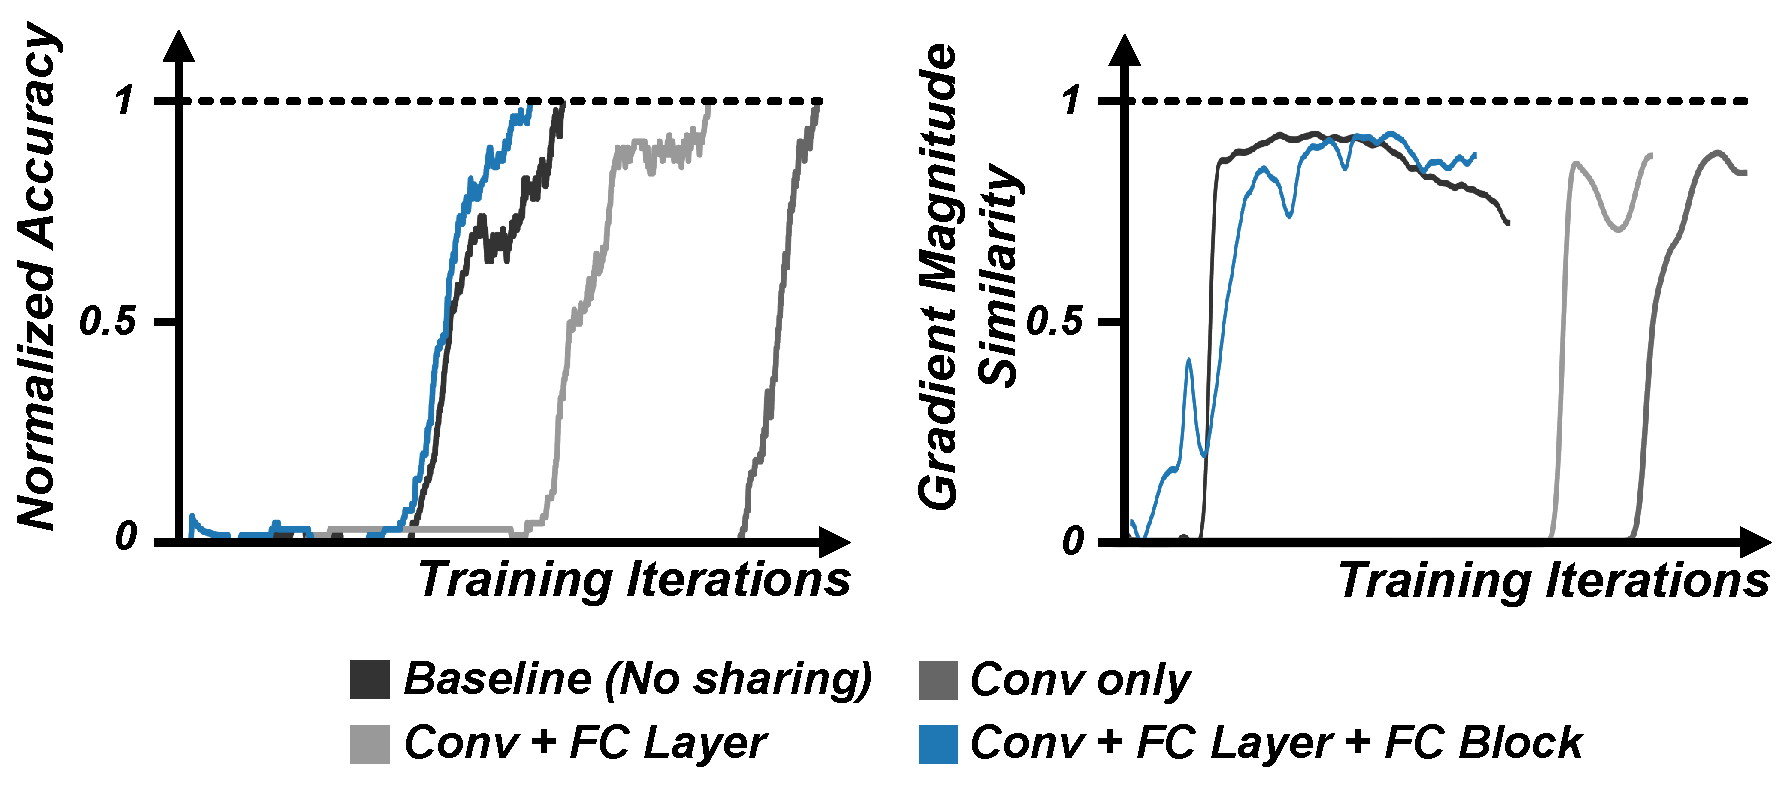
\includegraphics[width=0.95\linewidth]{Figures/Fig_ablation_study_v2.pdf}\\
  \caption{Training performance vs. gradient magnitude similarity.}\label{fig:ablation_study}
   \end{center}
   \vspace{-0.5cm}
\end{figure}

\begin{equation}
\label{eq_GMS}
\Phi(\boldsymbol{g_i, g_j})={{2||\boldsymbol{g_i}||_2}{||\boldsymbol{g_j}||_2}\over{{||\boldsymbol{g_i}||_2^2}{||\boldsymbol{g_j}||_2^2}}}
\end{equation}
quantifies the similarity of gradient magnitudes between two different neural networks. A value of 1 indicates perfect agreement, while lower values reflect increasing disparity.

The results in Fig. \ref{fig:ablation_study} show a strong correlation between normalized accuracy and gradient magnitude similarity. In particular, for partial sharing configurations such as Conv-only sharing and Conv + FC Layer sharing, a larger number of training iterations is required before the gradient magnitude similarity increases, leading to slower convergence compared to the other configurations. These results indicate that, compared to sharing all layers, partial sharing schemes such as Conv-only or Conv + FC Layer sharing can make it more difficult to align the gradient magnitudes between the actor and critic networks. As a consequence, these schemes tend to require a greater number of training iterations for the convergence.

\begin{figure}[!t]
\centering

\subfloat[]{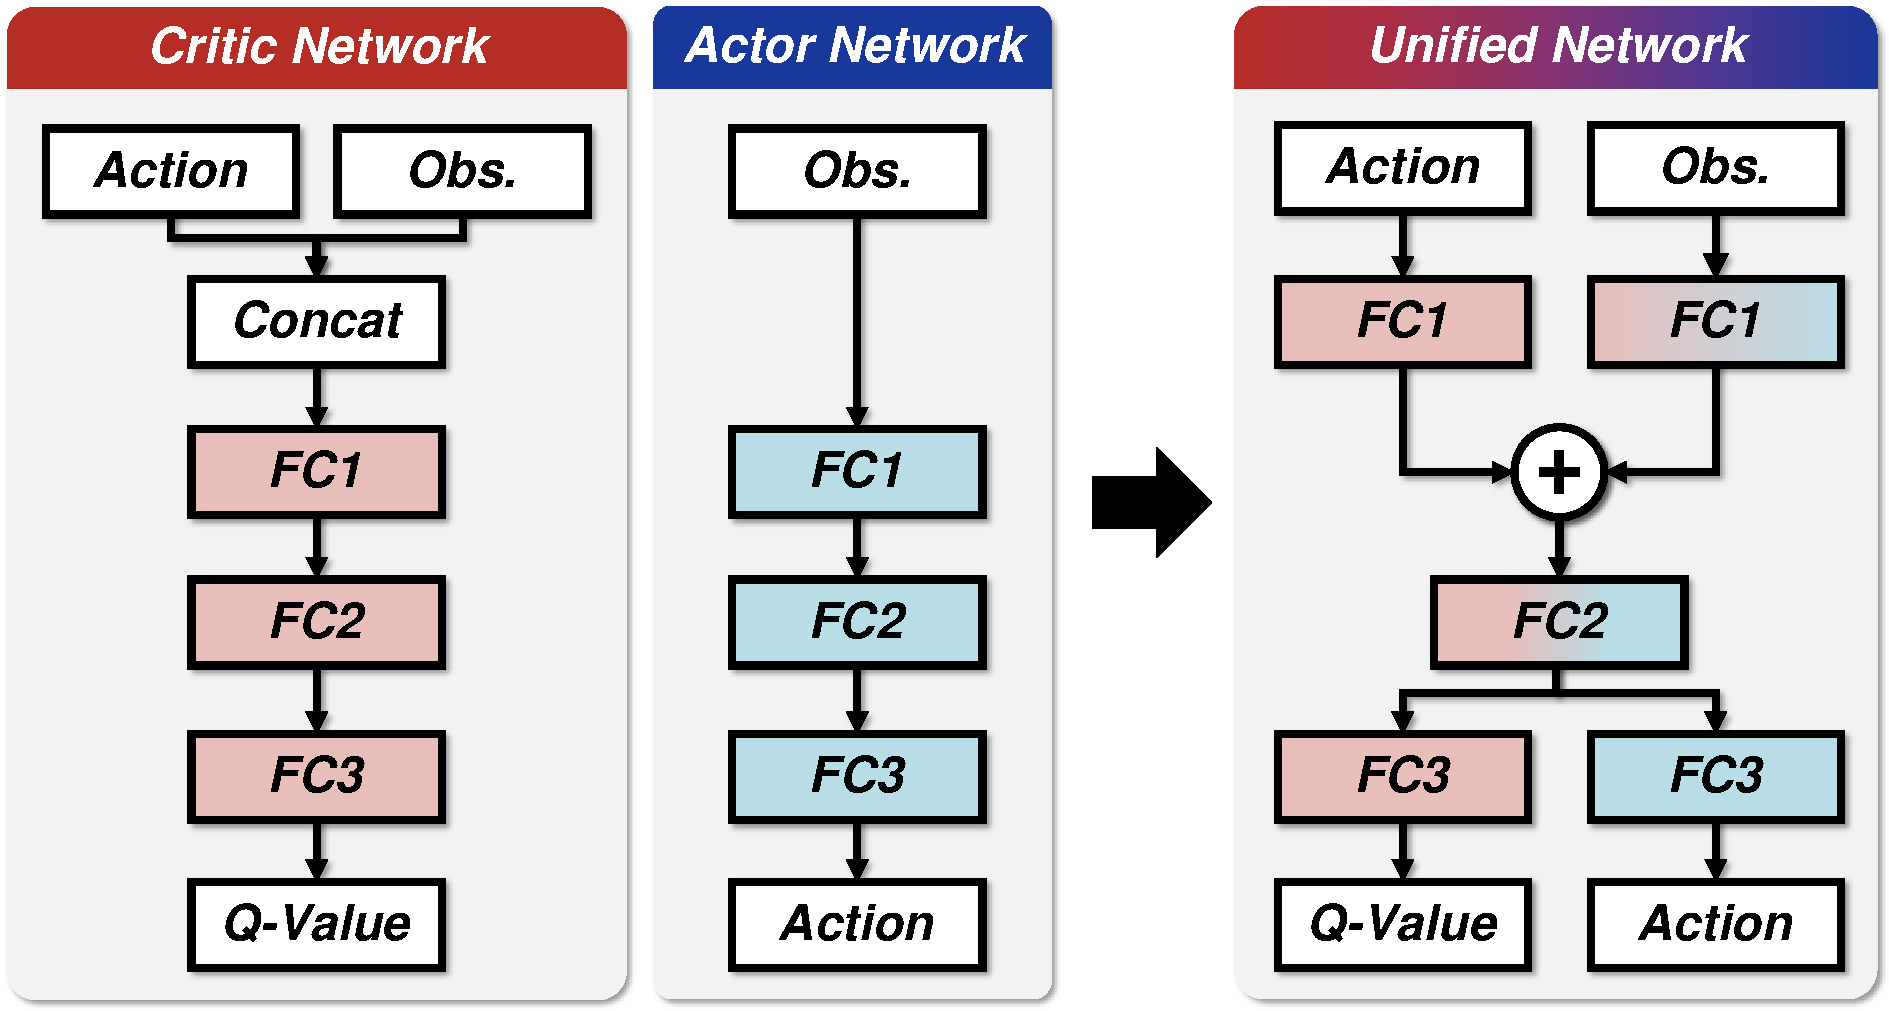
\includegraphics[width=1\linewidth]{Figures/Fig_single_critic.pdf}\label{fig:single_critic}}

\subfloat[]{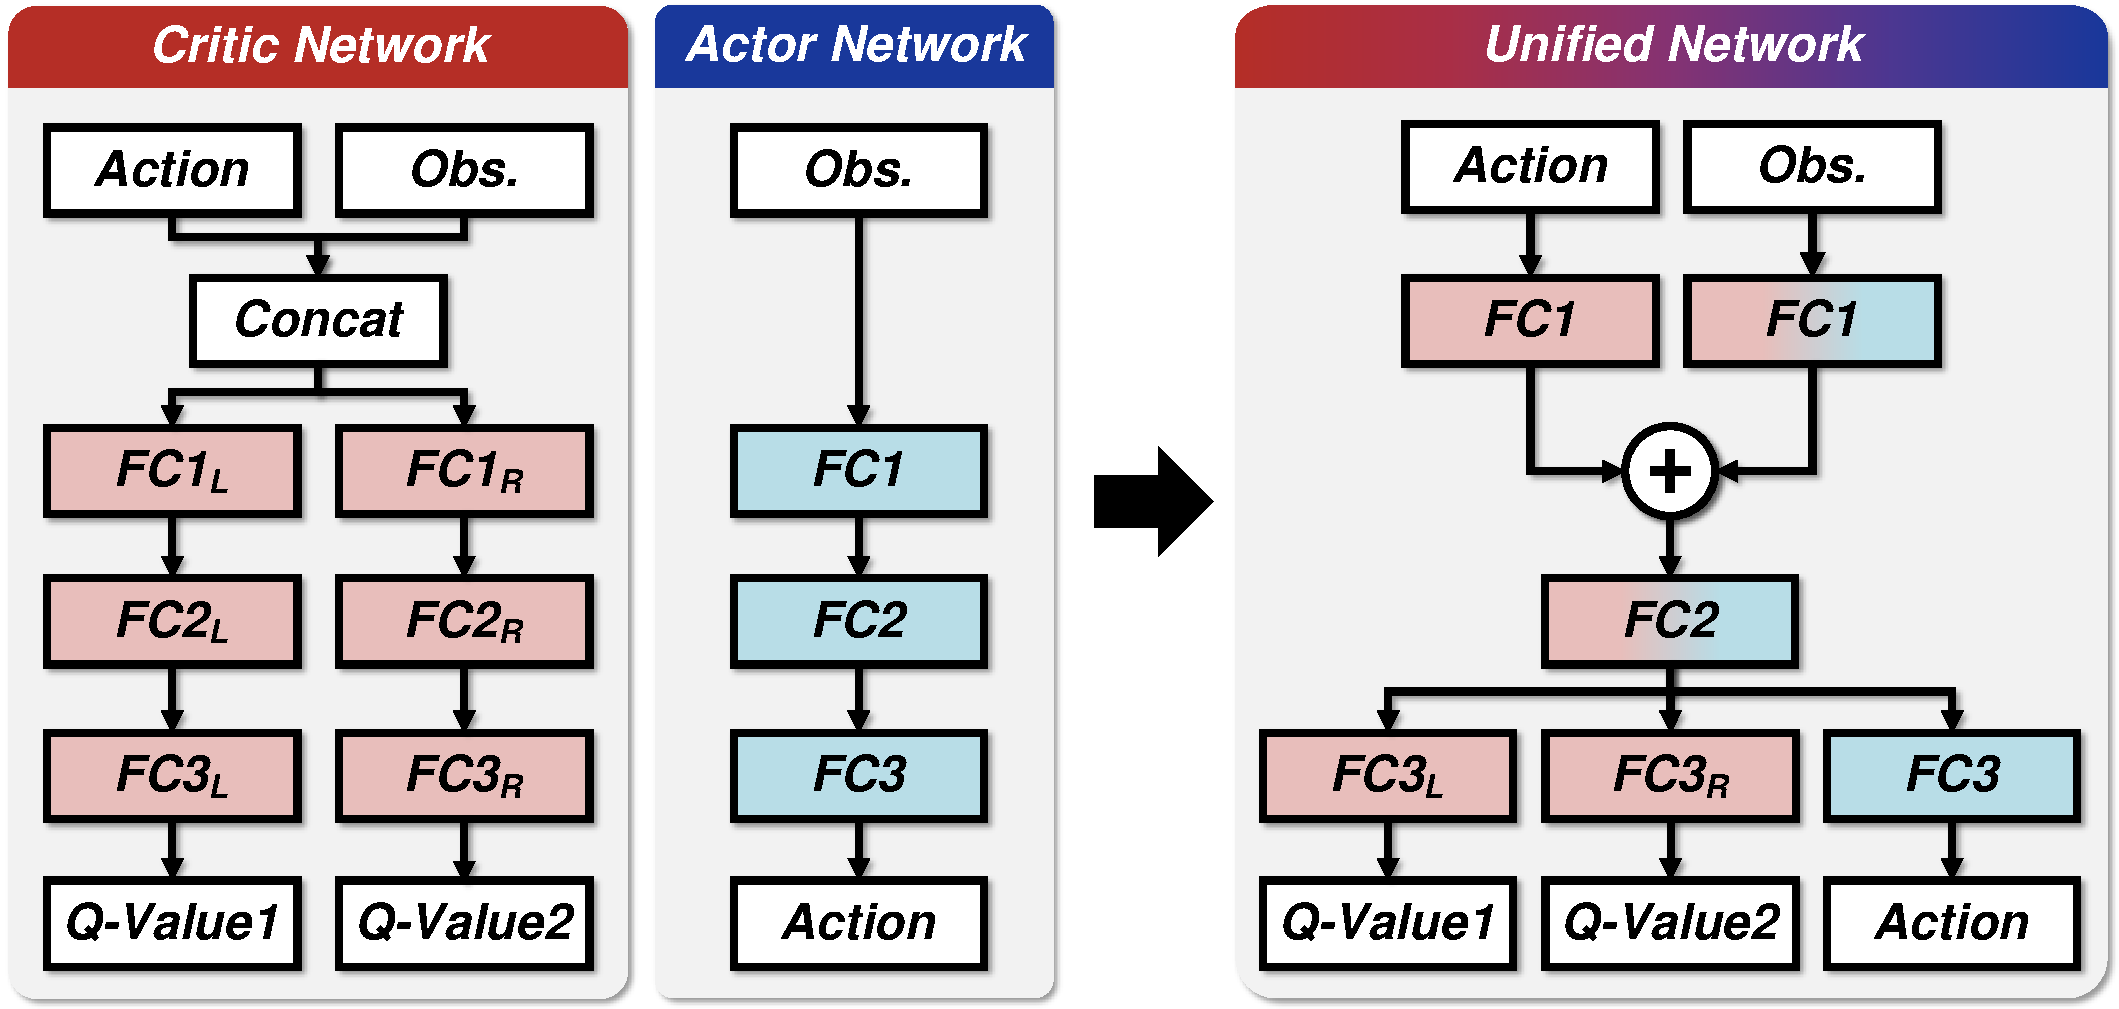
\includegraphics[width=1\linewidth]{Figures/Fig_double_critic.pdf}\label{fig:double_critic}}

\caption{Applying unified network architecture to (a) single-critic and (b) double-critic networks.}\label{fig:network_architecture_expansion}
\vspace{-0.5cm}
\end{figure}

We suggest that the unified network remains effective since the actor and critic largely rely on a common state representation, with task-specific variations absorbed by lightweight, decoupled heads. This is consistent with multi-task learning behavior, where early and mid-level features are shared while the output branches are specialized \cite{mtl1, mtl2}. Fig. \ref{fig:ablation_study} shows that, although GMS is low at the beginning of training, both GMS and normalized accuracy increase simultaneously, indicating progressive alignment of the shared representation. Moreover, the proposed unified architecture can be viewed as a form of multi-task learning in which shared layers serve both actor and critic while lightweight heads capture task-specific variations. It should be noted that, however, effectiveness may depend on gradient alignment and environment specifics; the proposed approach was proven effective for the autonomous navigation task considered in this work.


\subsection{Generalization to Other RL Algorithms}


Up to this point, the unified network architecture has been evaluated only with D4PG. However, this approach is also directly applicable to other actor-critic-based algorithms as well. To experimentally validate its generality, we applied the sharing scheme to widely used DRL algorithms, including DDPG\cite{DDPG}, TD3\cite{TD3}, and SAC\cite{SAC}. DDPG adopts a single-critic network architecture, similar to D4PG, and can be implemented with the unified network as shown in Fig. \ref{fig:network_architecture_expansion}\subref{fig:single_critic}. In contrast, TD3 and SAC utilize double-critic network architectures, for which the unified network can be constructed as depicted in Fig. \ref{fig:network_architecture_expansion}\subref{fig:double_critic}.

\begin{figure}[!t]
\centering

% --- 왼쪽 열 시작 ---
\begin{minipage}{0.48\linewidth}
    \centering
    \subfloat[]{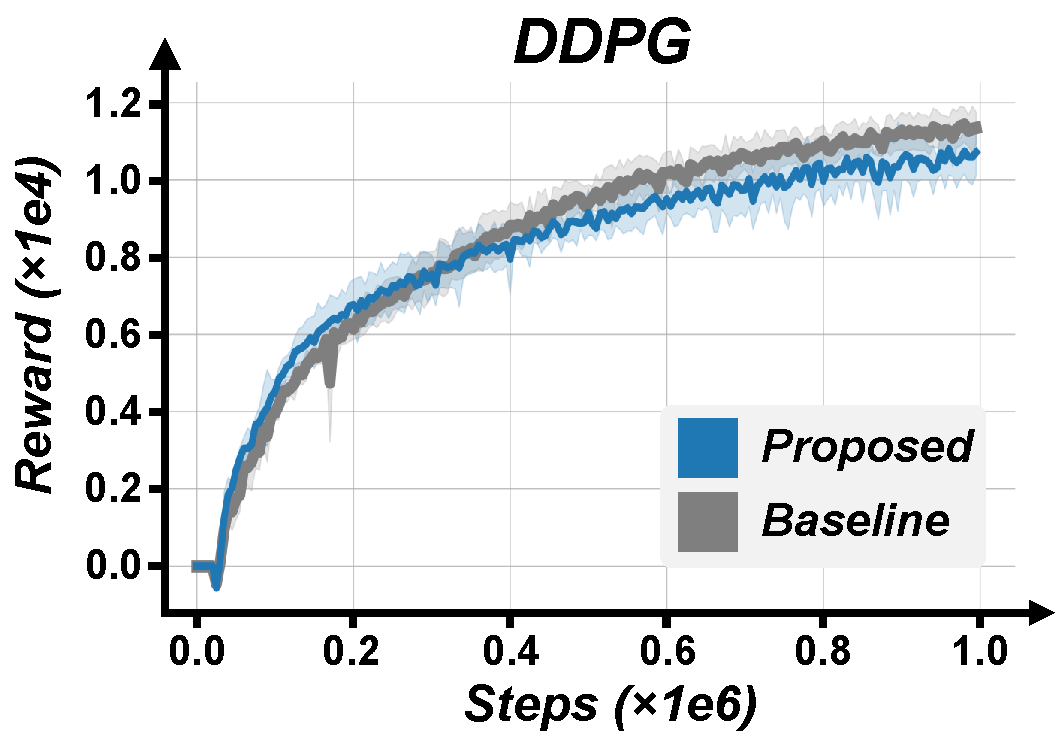
\includegraphics[width=\linewidth]{Figures/Fig_DDPG_v3.pdf}\label{fig:DDPG}} \\
    \subfloat[]{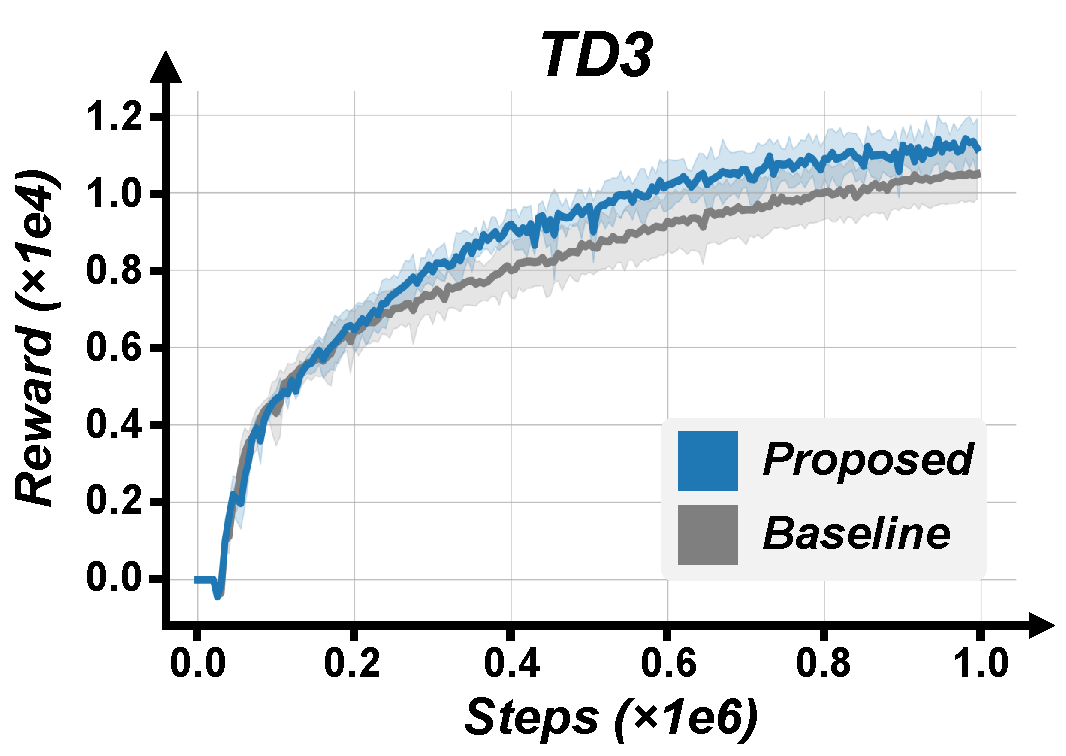
\includegraphics[width=\linewidth]{Figures/Fig_TD3_v3.pdf}\label{fig:TD3}} \\
    \subfloat[]{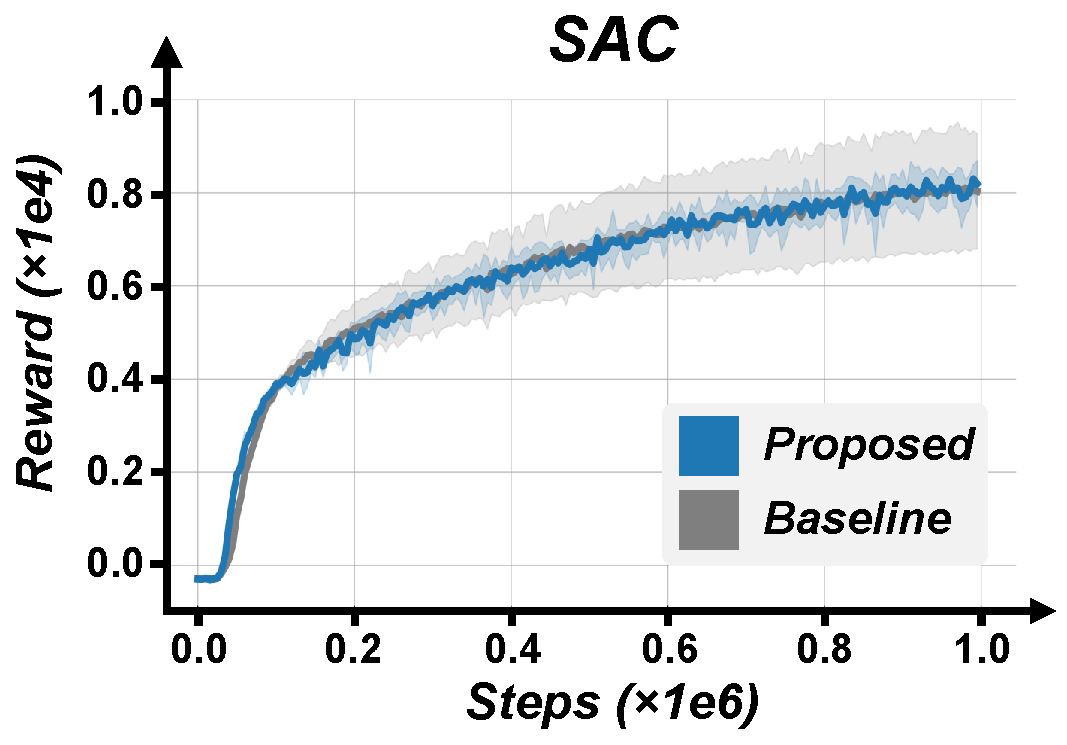
\includegraphics[width=\linewidth]{Figures/Fig_SAC_v3.pdf}\label{fig:SAC}}
\end{minipage}% <--- 두 minipage 사이의 불필요한 공백을 막기 위해 %를 붙입니다.
% --- 왼쪽 열 끝 / 오른쪽 열 시작 ---
\begin{minipage}{0.48\linewidth}
    \centering
    \subfloat[]{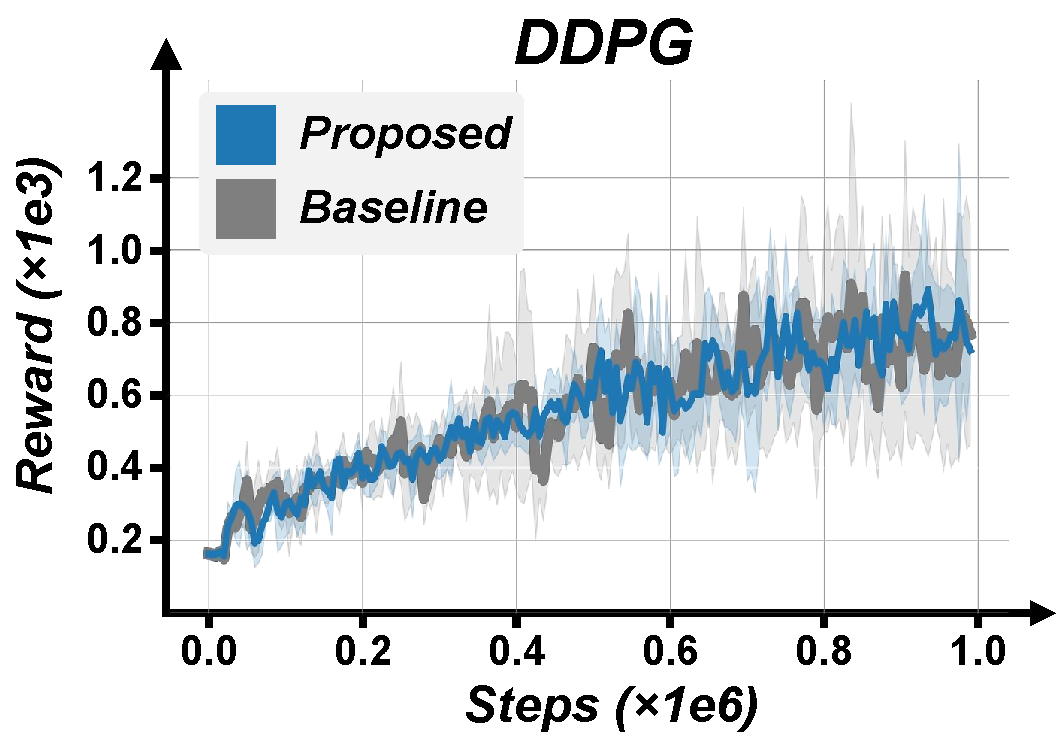
\includegraphics[width=\linewidth]{Figures/Fig_DDPG_humanoid_cropped.pdf}\label{fig:DDPG_Humanoid}} \\
    \subfloat[]{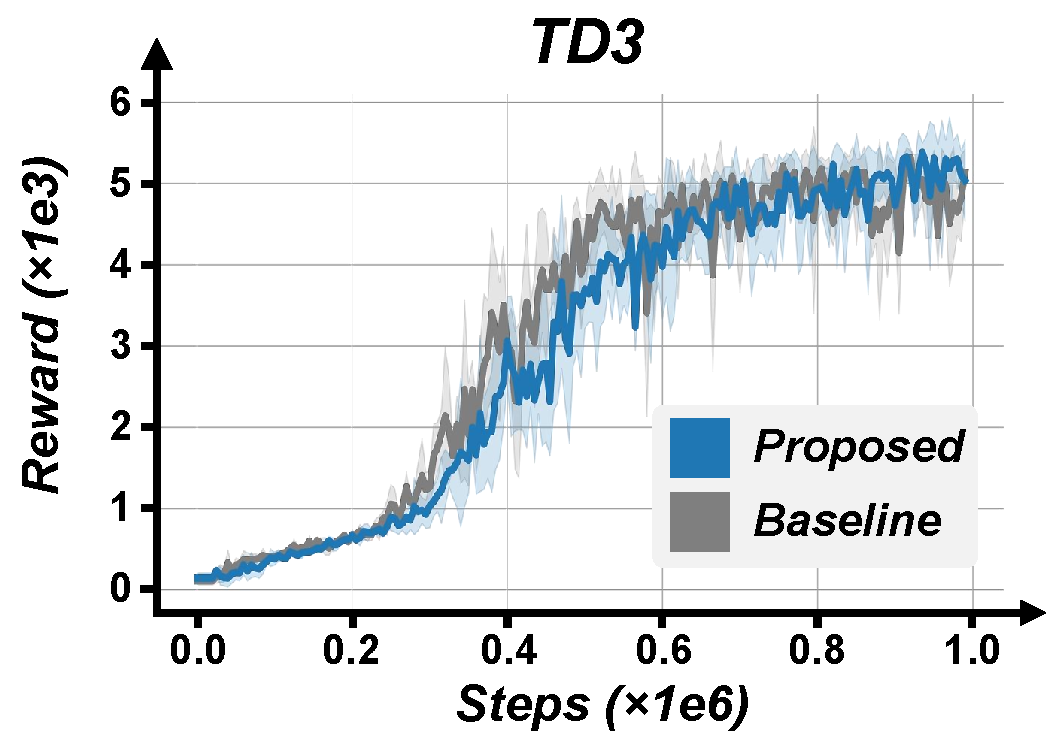
\includegraphics[width=\linewidth]{Figures/Fig_TD3_humanoid_cropped.pdf}\label{fig:TD3_Humanoid}} \\
    \subfloat[]{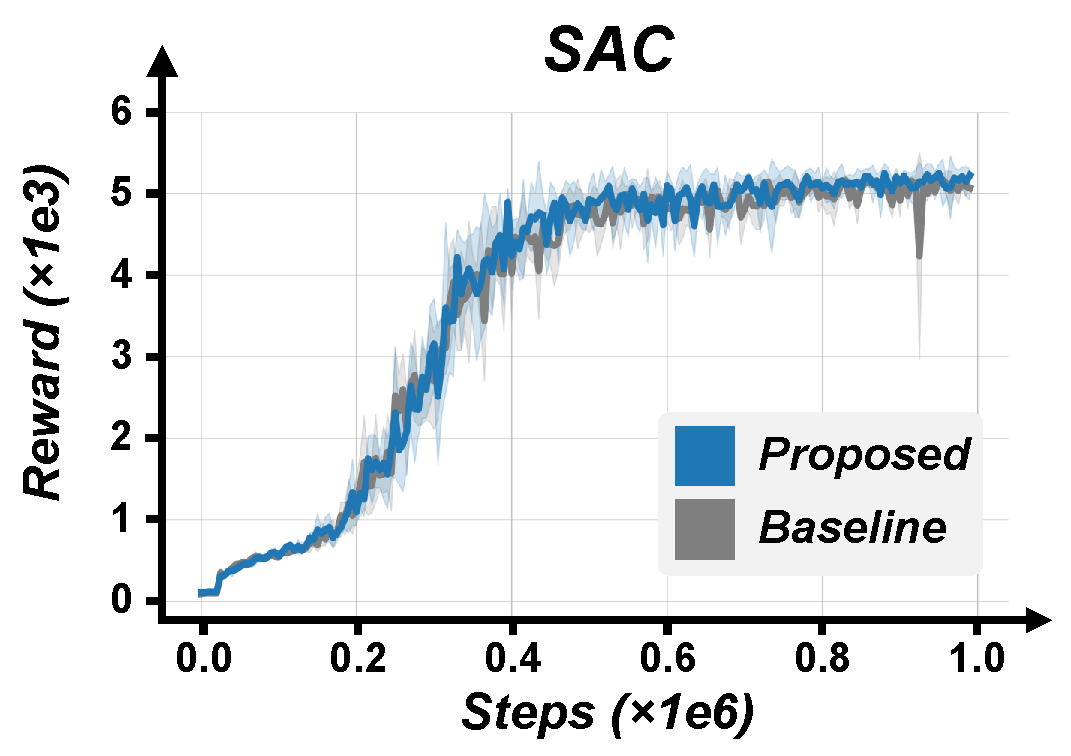
\includegraphics[width=\linewidth]{Figures/Fig_SAC_humanoid_cropped.pdf}\label{fig:SAC_Humanoid}}
\end{minipage}
% --- 오른쪽 열 끝 ---

\caption{Performance comparisons in HalfCheetah-v2 ((a)-(c)) and Humanoid-v2 ((d)-(f)) for different RL algorithms.}\label{fig:algorithm_experiment}
\vspace{-0.2cm}
\end{figure}

Fig. \ref{fig:algorithm_experiment} displays the learning curves for each algorithm representing the mean and one $\sigma$ range over five experiments with different random seeds. Experiments were conducted in the Halfcheetah-v2 and Humanoid-v2 environments of MuJoCo \cite{mujoco}. For Humanoid-v2, we additionally applied a gradient conflict mitigation technique (PCGrad) proposed in \cite{GMS}. PCGrad is a model-agnostic gradient-surgery method for multi-task learning. When two task gradients exhibit negative cosine similarity, it projects each gradient onto the other's normal plane to remove the conflicting component, which mitigates task interference and reduces sensitivity to curvature and gradient scale imbalance, improving the model's performance. Experimental results confirm that the proposed sharing scheme closely matches the non-shared baseline in all tasks and DRL algorithms. These results demonstrate that the proposed unified network architecture can be effectively applied to a wide range of actor-critic algorithms without compromising performance.

\section{Proposed DRL Processor} \label{sec:processor}
\subsection{Overall Architecture} \label{subsec:overall_arch}

\begin{figure}[!t]
   \begin{center}
   % \captionsetup{skip=-5pt}
  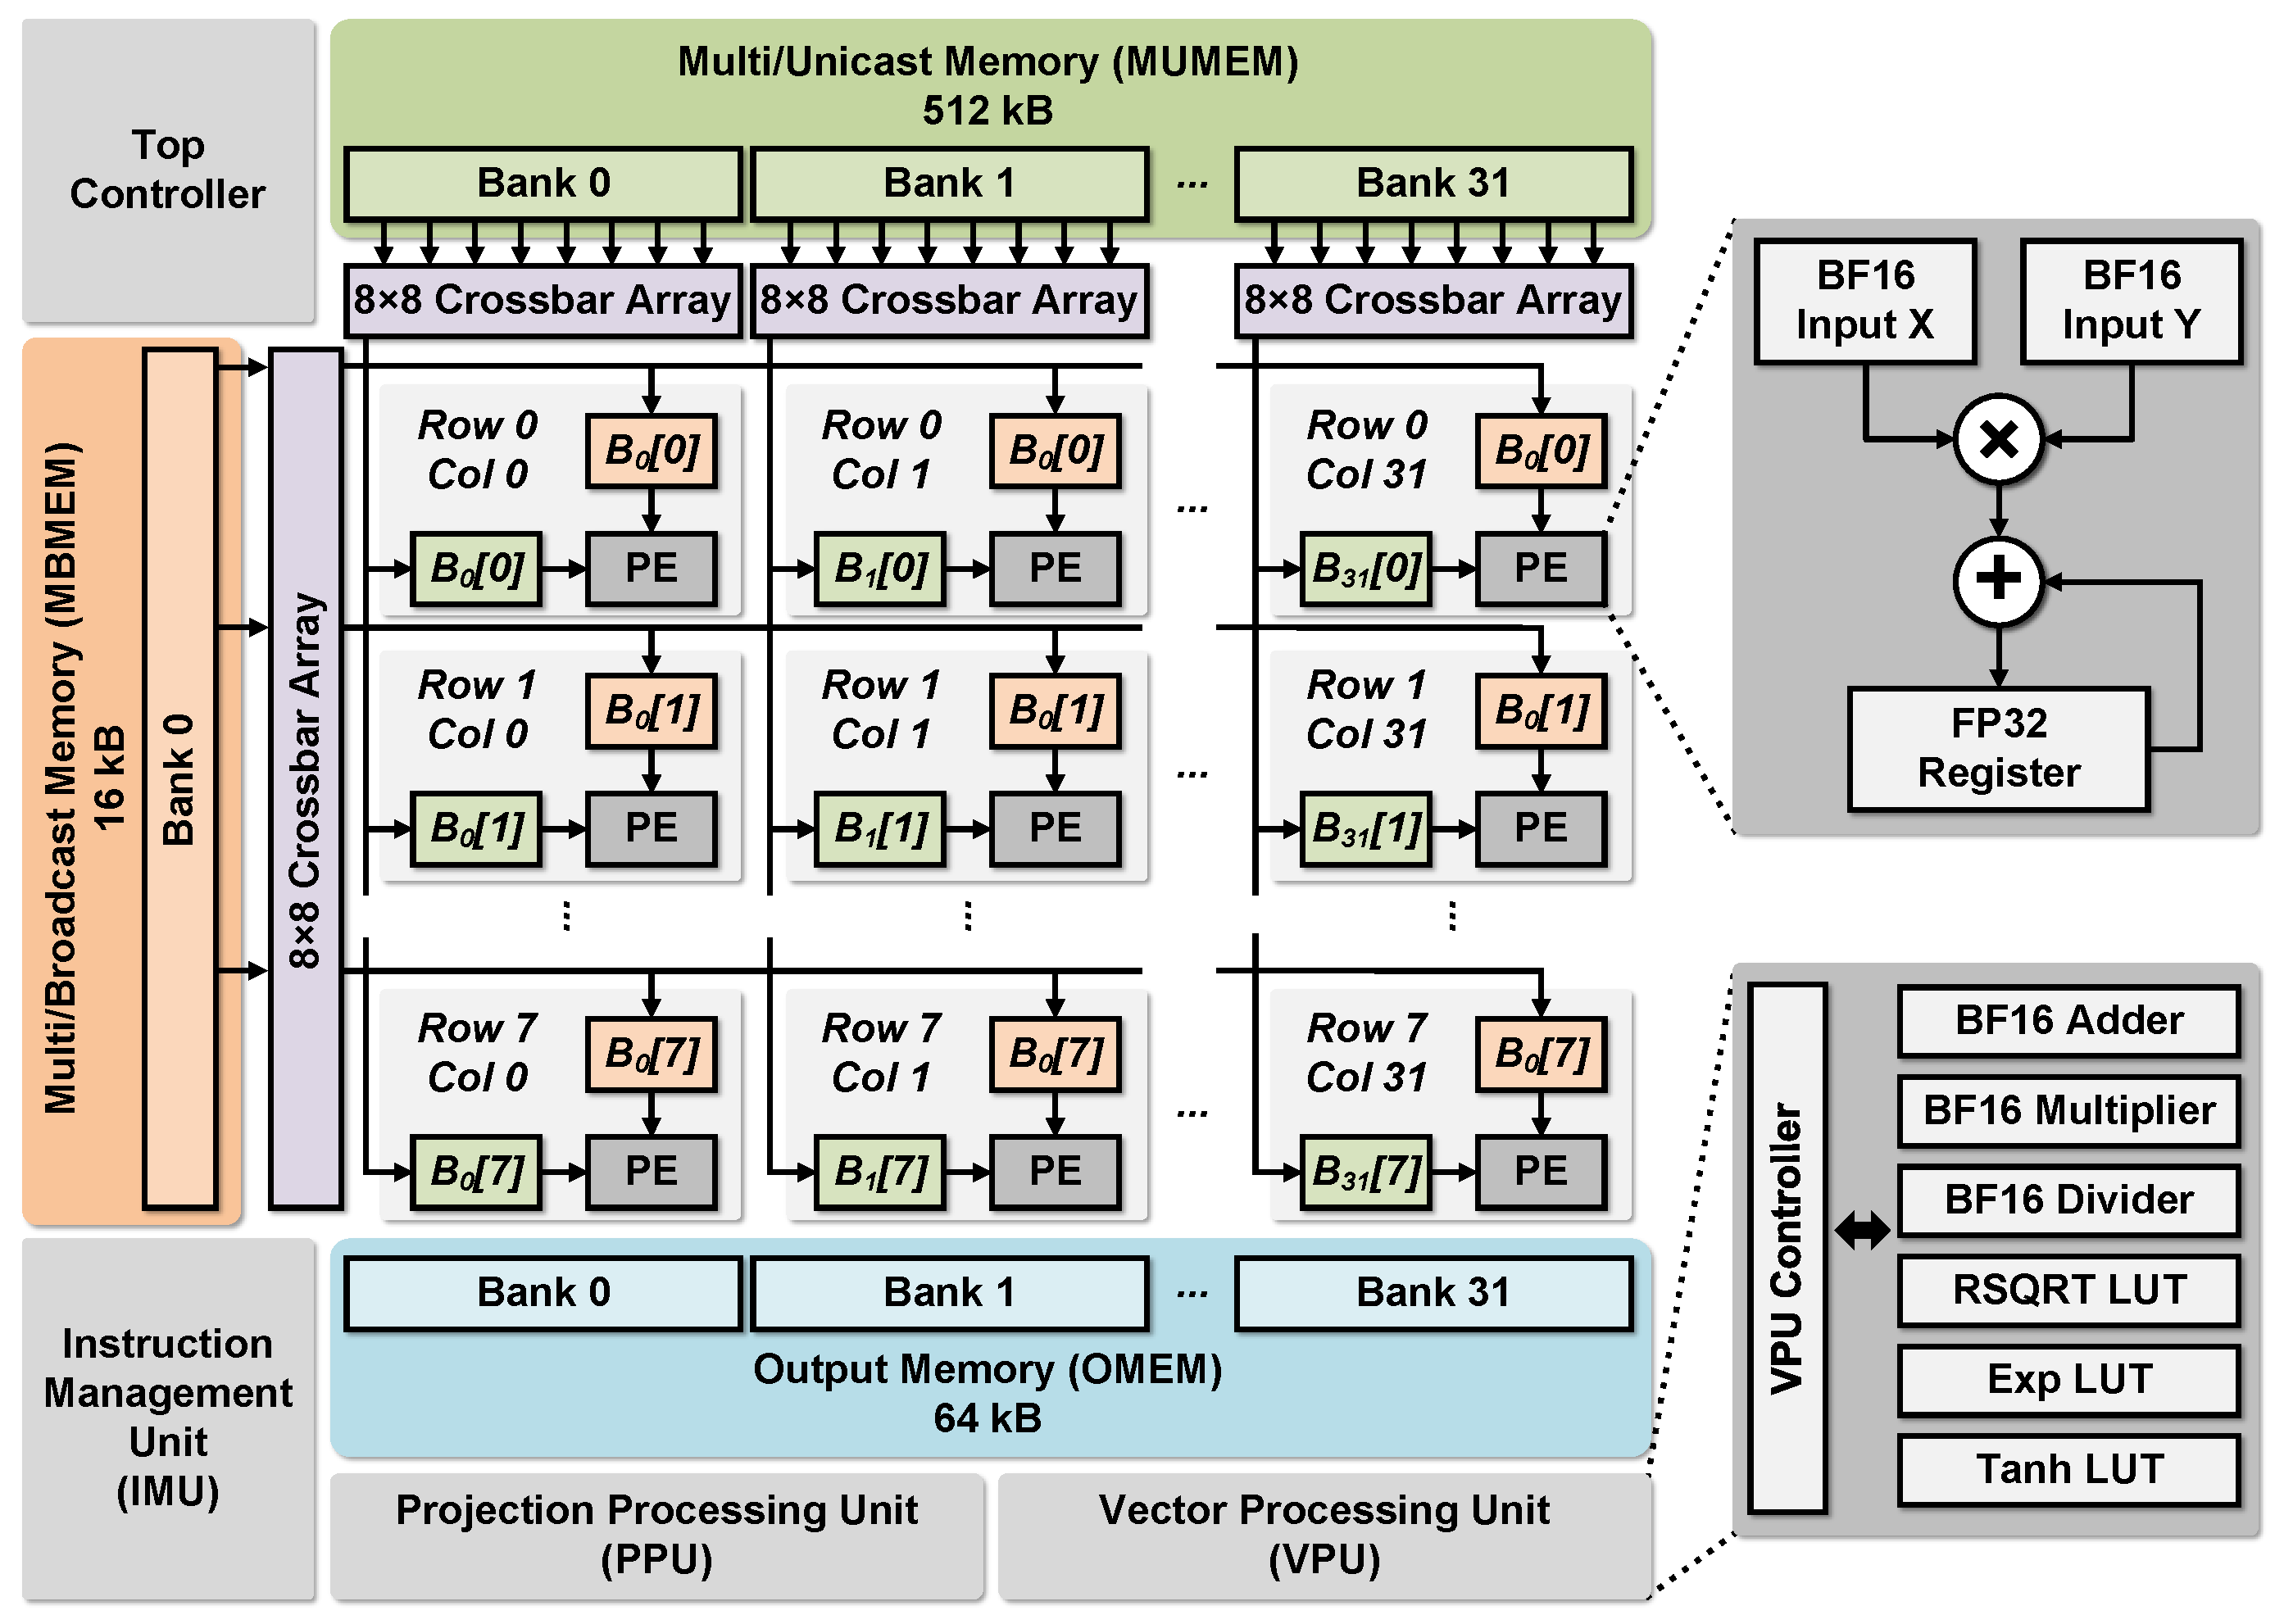
\includegraphics[width=1\linewidth]{Figures/Fig_architecture_rev1_v2_cropped.pdf}\\
 \caption{Overall architecture of proposed DRL processor.}\label{fig:overall_architecture}
   \end{center}
   \vspace{-0.8cm}
\end{figure}



\begin{figure}[!t]
\centering

\subfloat[]{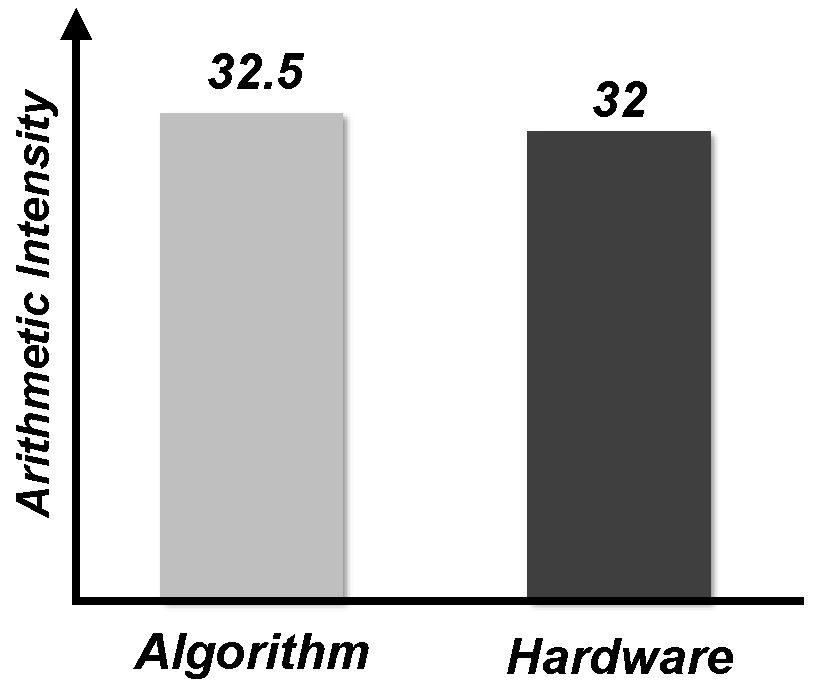
\includegraphics[width=0.5\linewidth]{Figures/Fig_arithmetic_intensity_v2.pdf}\label{fig:arithmetic_intensity}}
\subfloat[]{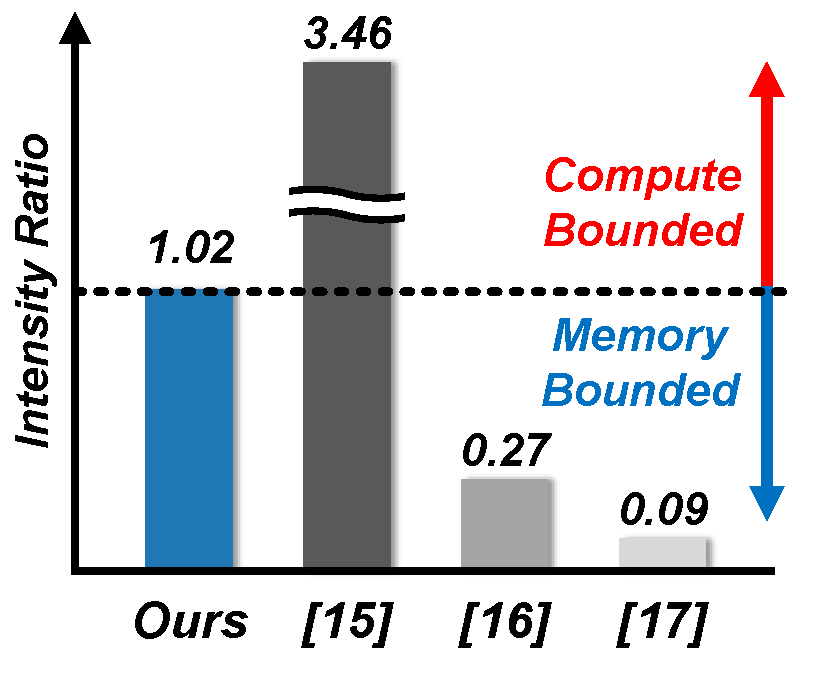
\includegraphics[width=0.5\linewidth]{Figures/Fig_arithmetic_intensity_comparison_rev1_v2_cropped.pdf}\label{fig:arithmetic_intensity_comparison}}

\caption{(a) Arithmetic intensity of algorithm and hardware in our design. (b) Arithmetic intensity ratio comparisons.}\label{fig:arithmetic_intensity_top}
\vspace{-0.5cm}
\end{figure}


Fig. \ref{fig:overall_architecture} illustrates the overall architecture of the proposed DRL processor. The processor consists of 8×32 processing element (PE) array, 16-kB Multi/Broadcast Memory (MBMEM), 512-kB Multi/Unicast Memory (MUMEM), 64-kB Output Memory (OMEM), an Instruction Management Unit (IMU), a Vector Processing Unit (VPU), a Projection Processing Unit (PPU), and a top-level controller with a 128-bit external I/O interface. 8$\times$8 crossbar arrays are placed at the output of MBMEM and MUMEM to enable flexible data distribution. MBMEM delivers data along rows of the PE array, so all PEs within the same row receive identical data. MUMEM delivers data along columns of the PE array, with each MUMEM bank mapped to a specific PE column and supplying data to that column. Each PE supports BF16 multiplication and FP32 accumulation for stable training. IMU orchestrates the inference and training executions by issuing appropriate instructions. VPU performs element-wise operations and supports non-linear activation functions including ReLU \cite{relu}, ELU \cite{elu} and Tanh. Non-linear functions such as reciprocal square root (RSQRT), exponential for ELU and softmax, and hyperbolic tangent function (Tanh) are implemented using LUTs. PPU is specifically designed to support categorical projection, which is essential for DistRL algorithms such as D4PG.

Arithmetic intensity \cite{operational_intensity}, defined as the ratio of total operations to data access for algorithms and the ratio of compute capability to external memory bandwidth for hardware, is a key metric for estimating hardware utilization. In addition, arithmetic intensity ratio is defined as the algorithmic arithmetic intensity divided by the hardware arithmetic intensity. A ratio close to 1 indicates that the hardware's compute throughput and external memory bandwidth are well matched to the algorithm. Any mismatch of these two leads to under-utilization of either compute resources or external memory bandwidth. To address this, the proposed design employs 256 PEs, carefully matching the algorithmic and hardware arithmetic intensity to the 128-bit external I/O bandwidth. As a result, the arithmetic intensity ratio becomes 1.02, as shown in Fig. \ref{fig:arithmetic_intensity_top}\subref{fig:arithmetic_intensity}, which is close to the ideal value of 1 and effectively prevents under-utilization of any hardware resource. This demonstrates a significant improvement in resource utilization compared to prior designs, as displayed in Fig. \ref{fig:arithmetic_intensity_top}\subref{fig:arithmetic_intensity_comparison}.

\begin{figure}[!t]
\centering

\subfloat[]{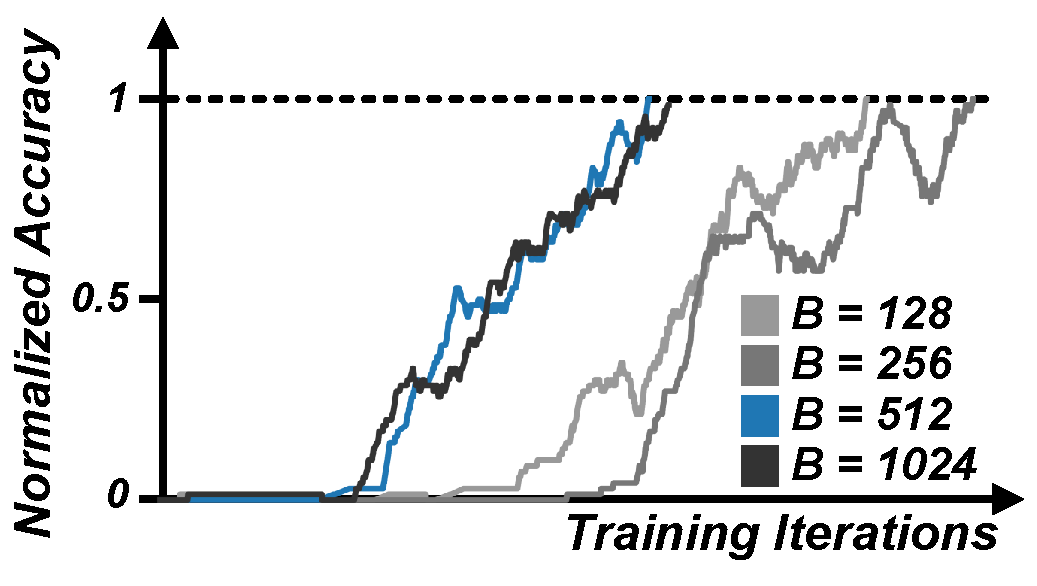
\includegraphics[width=0.58\linewidth]{Figures/Fig_batch_sweep_rev1_cropped.pdf}\label{fig:batch_sweep}}
\subfloat[]{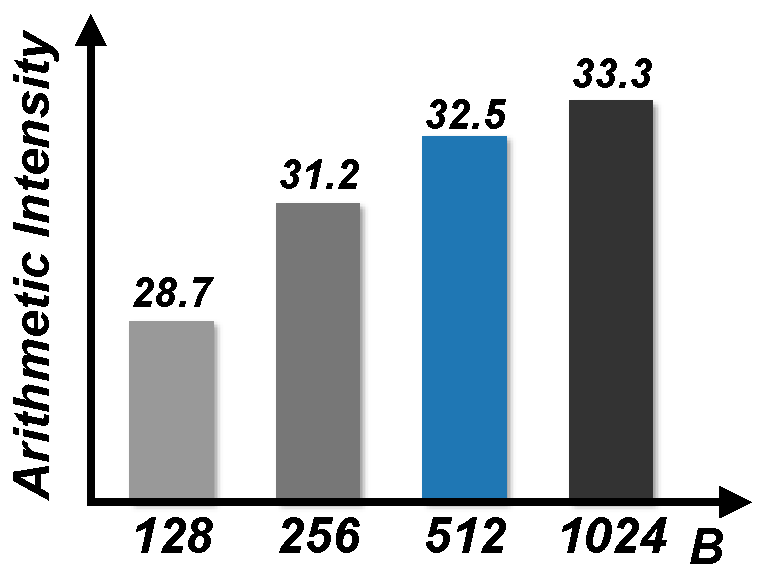
\includegraphics[width=0.43\linewidth]{Figures/Fig_batch_sweep_ai_rev1_cropped.pdf}\label{fig:batch_sweep_ai}}

\caption{(a) training performance and (b) arithmetic intensity vs. batch size (B).}\label{fig:batch_sweep_top}
\vspace{-0.5cm}
\end{figure}

\begin{figure}[!t]
\centering

\subfloat[]{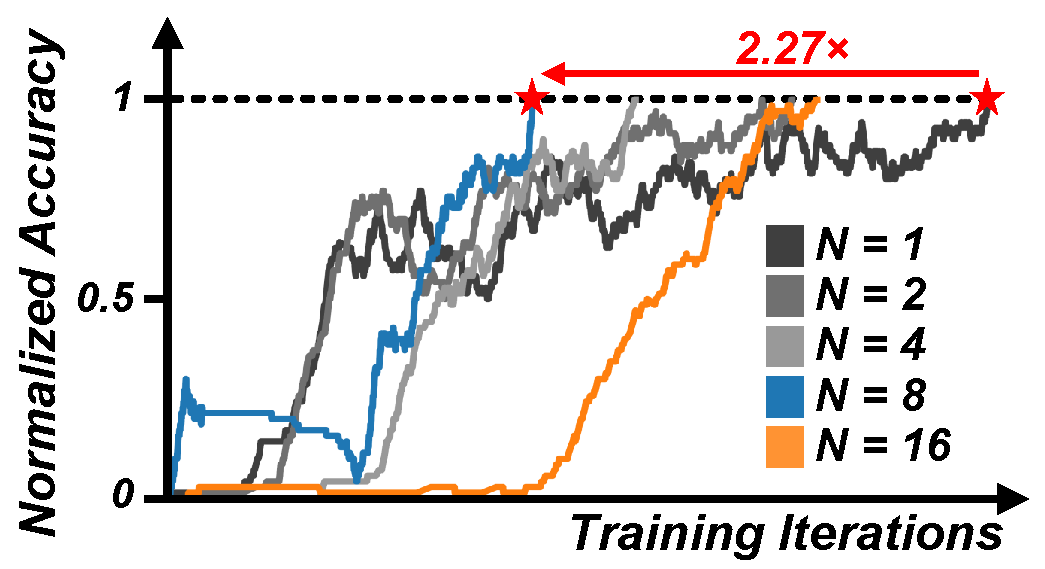
\includegraphics[width=0.6\linewidth]{Figures/Fig_sparse_training_rev1_v2_cropped.pdf}\label{fig:sparse_training}}
\subfloat[]{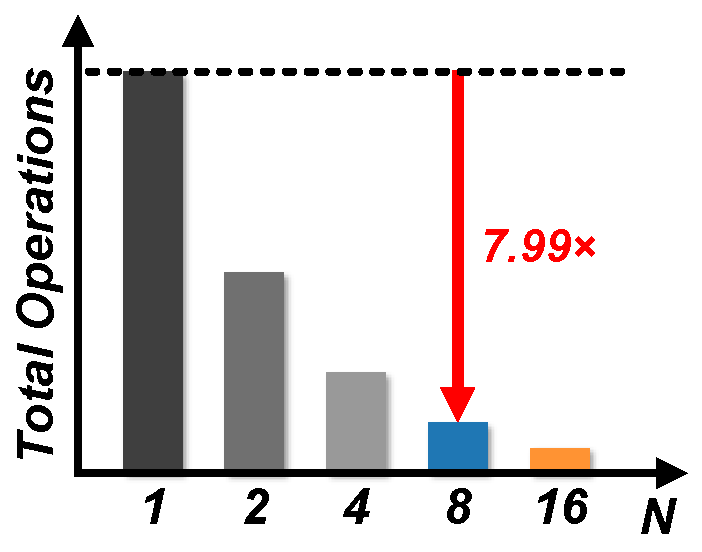
\includegraphics[width=0.4\linewidth]{Figures/Fig_sparse_training_ops_rev1_cropped.pdf}\label{fig:sparse_training_ops}}

\caption{(a) Training performance and (b) the number of training operations per iteration for various inference-to-training ratios.}\label{fig:sparse_training_top}
\vspace{-0.2cm}
\end{figure}

Fig. \ref{fig:batch_sweep_top}\subref{fig:batch_sweep} shows the training performance across batch sizes. Using relatively smaller batch sizes (e.g., 128 and 256) exhibit slower training convergence. Batch sizes of 512 and 1024 achieve similar training performance, but a batch size of 1024 requires twice the number of operations and external-memory accesses compared to batch size of 512. In addition, Fig. \ref{fig:batch_sweep_top}\subref{fig:batch_sweep_ai} shows that the model’s arithmetic intensity increases with batch size but quickly saturates. Beyond our design point of 512 batch size, adding more PEs to meet real-time constraints raises compute throughput without improving arithmetic intensity, leaving the workload memory-bound under a fixed I/O bandwidth budget and incurring power and area overheads. Therefore, our design choice of 512 batch size represents an optimal trade-off between training performance and hardware efficiency.

\subsection{Inference-on-Request (IoR) Scheduling}

In \cite{sparse_training}, it was shown that sparse training, where training is performed less frequently than inference, can lead to improved performance over conventional dense training. The inference-to-training ratio, $N$, is defined as the number of inference steps performed between each training iteration. For example, $N=4$ indicates that four inference steps are conducted for every training iteration. Fig. \ref{fig:sparse_training_top}\subref{fig:sparse_training} shows that increasing the inference-to-training ratio reduces the number of iterations required for convergence compared to dense training ($N=1$). The fastest convergence was achieved at $N=8$, while a further increase to $N=16$ resulted in slower convergence due to infrequent training iterations. In addition, Fig. \ref{fig:sparse_training_top}\subref{fig:sparse_training_ops} demonstrates that the number of training operations per iteration also decreases with larger inference-to-training ratios. Based on these observations, the inference-to-training ratio was set to 8 in our design, which reduced the required training iterations and the number of training operations per iteration by 2.27$\times$ and 7.99$\times$, respectively, compared to conventional dense training. As a result, the total number of operations required for training convergence is reduced by 18.14$\times$.

\begin{figure}[!t]
   \begin{center}
  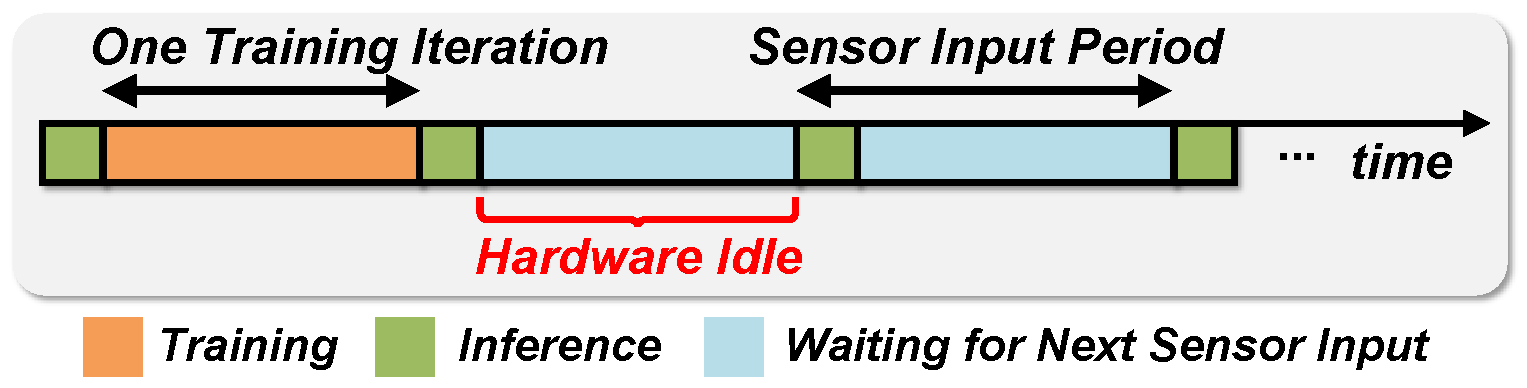
\includegraphics[width=0.95\linewidth]{Figures/Fig_conventional_scheduling_v3.pdf}\\
  \caption{Conventional sequential scheduling for sparse training.}\label{fig:conventional_scheduling}
   \end{center}
   \vspace{-0.8cm}
\end{figure}

However, sparse training with conventional sequential scheduling inevitably incurs hardware idle time as depicted in Fig. \ref{fig:conventional_scheduling}. Since inference and control are synchronized with the sensor input period, the computationally intensive training must be completed within each sensor input period. Consequently, the processor must operate at a high clock frequency to meet the throughput requirement, and the hardware remains idle between inference until the next training is required.

\begin{figure}[!t]
   \begin{center}
  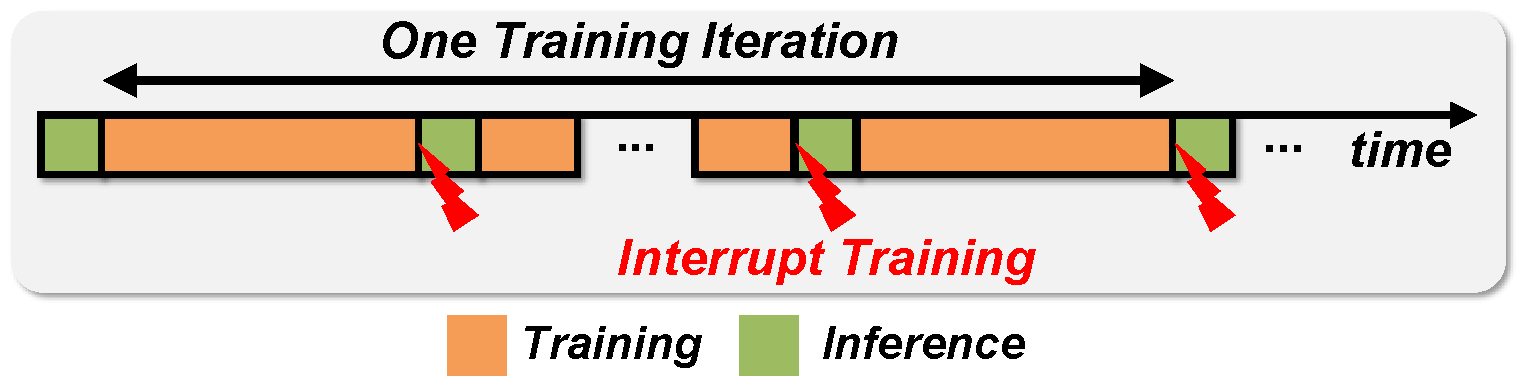
\includegraphics[width=0.95\linewidth]{Figures/Fig_ior_scheduling_v3.pdf}\\
  \caption{Proposed IoR scheduling.}\label{fig:ior_scheduling}
   \end{center}
   \vspace{-0.5cm}
\end{figure}



The fundamental limitation of conventional sequential scheduling arises from executing both training and inference on the same core in a strictly sequential manner. To address this, a recent design in \cite{CICC25} introduced separate cores dedicated to training and inference. While this scheme sustains high utilization for the training core, the inference core inherently suffers from low utilization due to environment response time. Additionally, as training and inference are performed on separate cores, simultaneous external memory accesses can lead to bus contention, which can cause one core to stall while the other completes its access. In addition, this architecture cannot be easily optimized for a wide range of inference-to-training ratios; as the ratio changes, the utilization of one of the cores inevitably decreases, limiting flexibility to support various scenarios.

\begin{figure}[!t]
   \begin{center}
  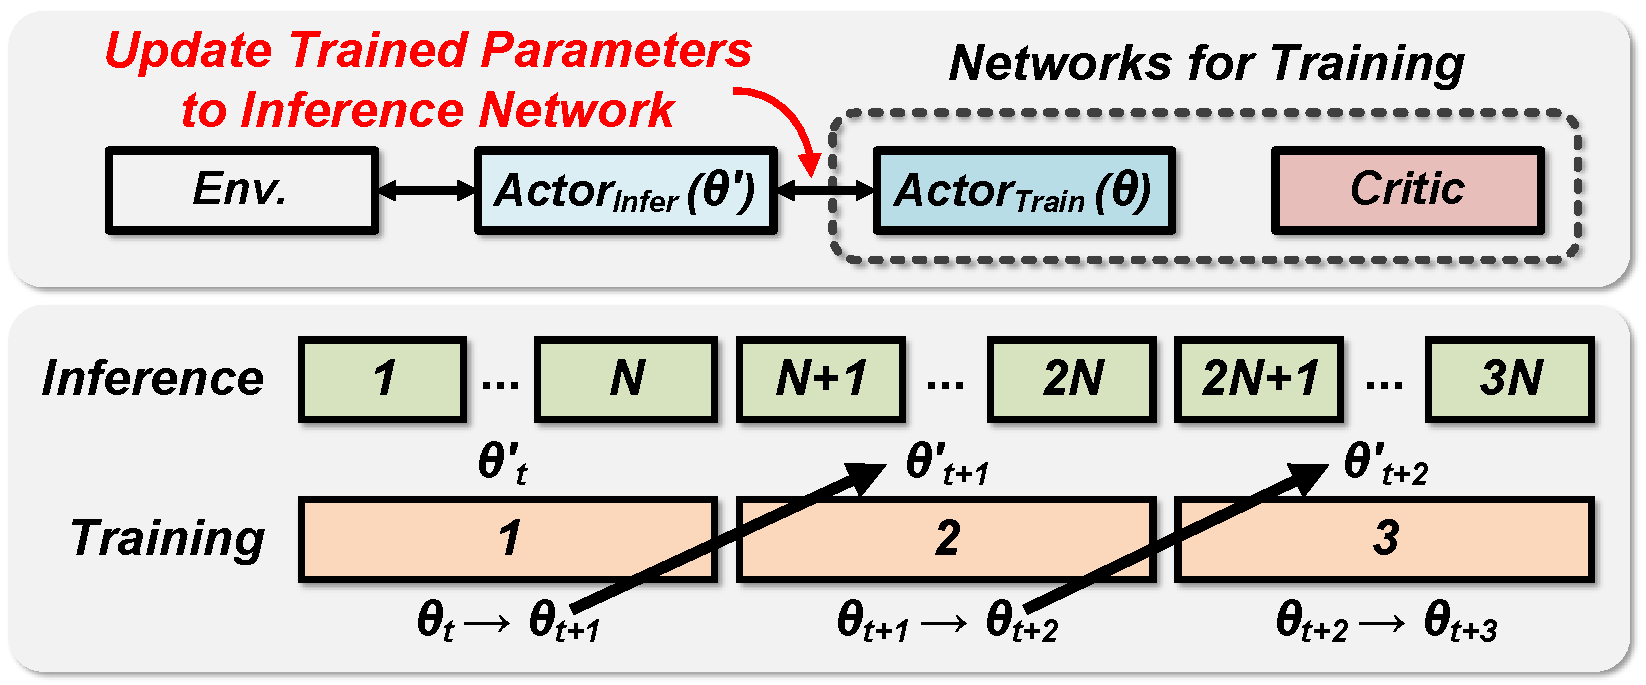
\includegraphics[width=0.95\linewidth]{Figures/Fig_ior_param_copy.pdf}\\
  \caption{Parameter copying between main actor network and inference actor network.}\label{fig:ior_param_copy}
   \end{center}
   \vspace{-0.5cm}
\end{figure}

\begin{figure}[!t]
   \begin{center}
  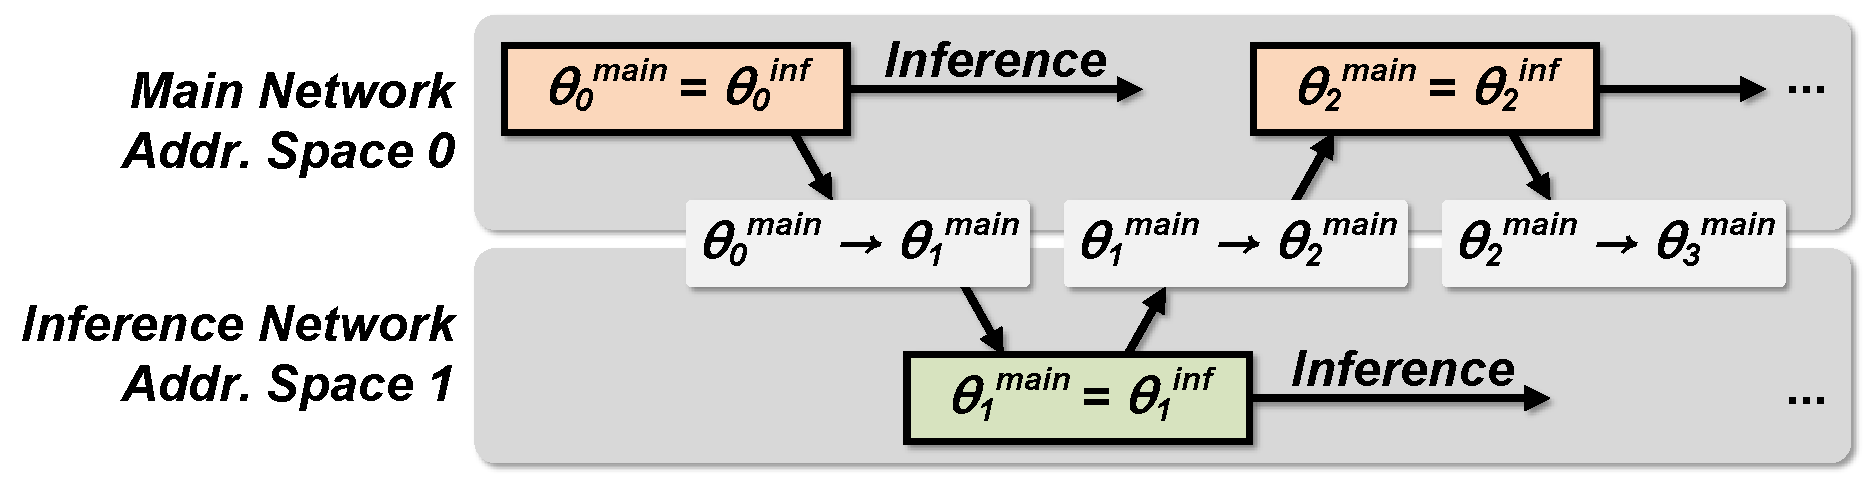
\includegraphics[width=1\linewidth]{Figures/Fig_address_pointer_rev1_cropped.pdf}\\
  \caption{Address pointer management scheme.}\label{fig:address_pointer}
   \end{center}
   \vspace{-0.8cm}
\end{figure}

To address these limitations, we propose an Inference-on-Request (IoR) scheduling scheme, which is described in Fig. \ref{fig:ior_scheduling}. In this scheme, computationally intensive training is executed in the background, while inference requests from the robot are given higher priority over training. Upon receiving an inference request, the processor temporarily suspends the ongoing training and immediately processes the inference task. Since each training iteration needs to be completed only before the next update is required, the processor can operate with a significantly lower clock frequency.


Since IoR scheduling allows inference to be performed without waiting for training to complete, there may be cases where inference is requested while the actor network is being updated. This could potentially result in unstable actions. To prevent this, a dedicated actor network is maintained for inference as shown in Fig. \ref{fig:ior_param_copy}. After each training iteration, the updated parameters of the actor network are copied to the inference network. Since directly copying parameters from external memory could incur significant power and latency overheads, we implement parameter synchronization using address pointers rather than duplicating the actual data as shown in Fig. \ref{fig:address_pointer}. Both the inference and main actor networks read parameters from the same address space. While main network is updated, write operations are redirected to an alternate address space in a ping-pong fashion. By simply switching the address pointer, unnecessary memory copies can be avoided, minimizing the overheads.

\begin{figure}[!t]
\centering

\subfloat[]{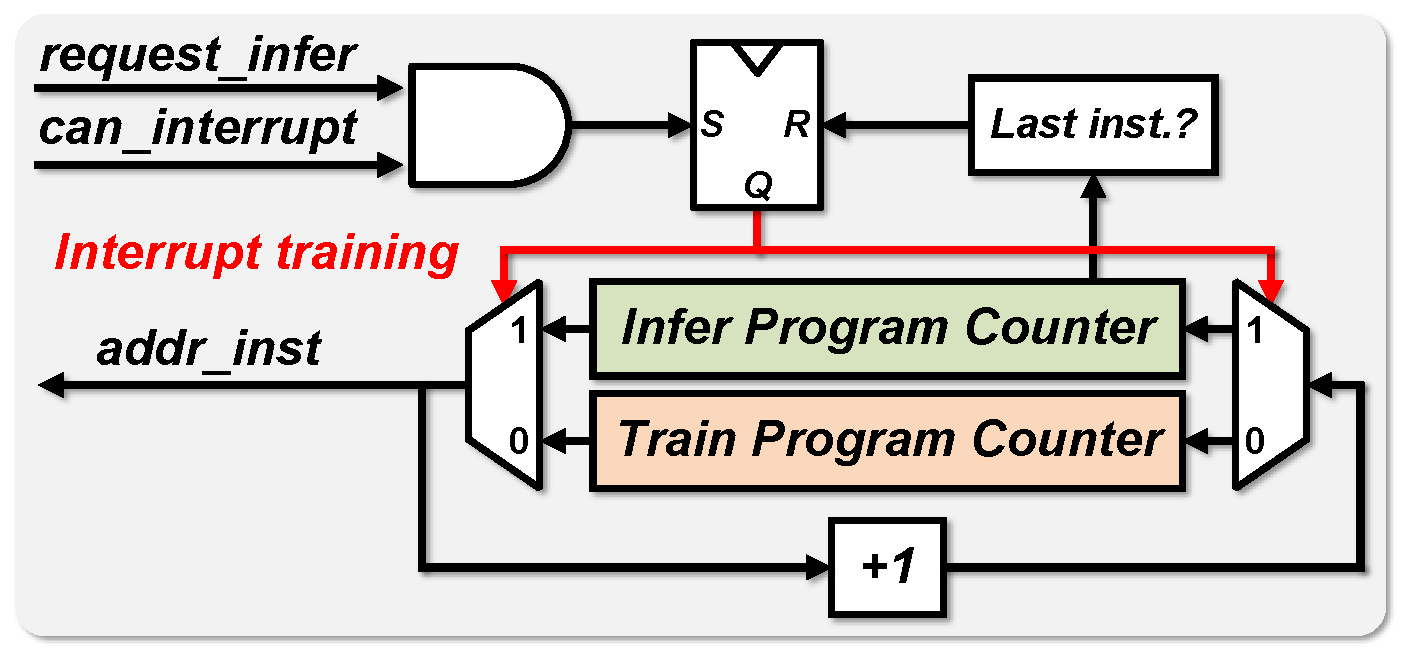
\includegraphics[width=0.9\linewidth]{Figures/Fig_IMU.pdf}\label{fig:IMU}}

\subfloat[]{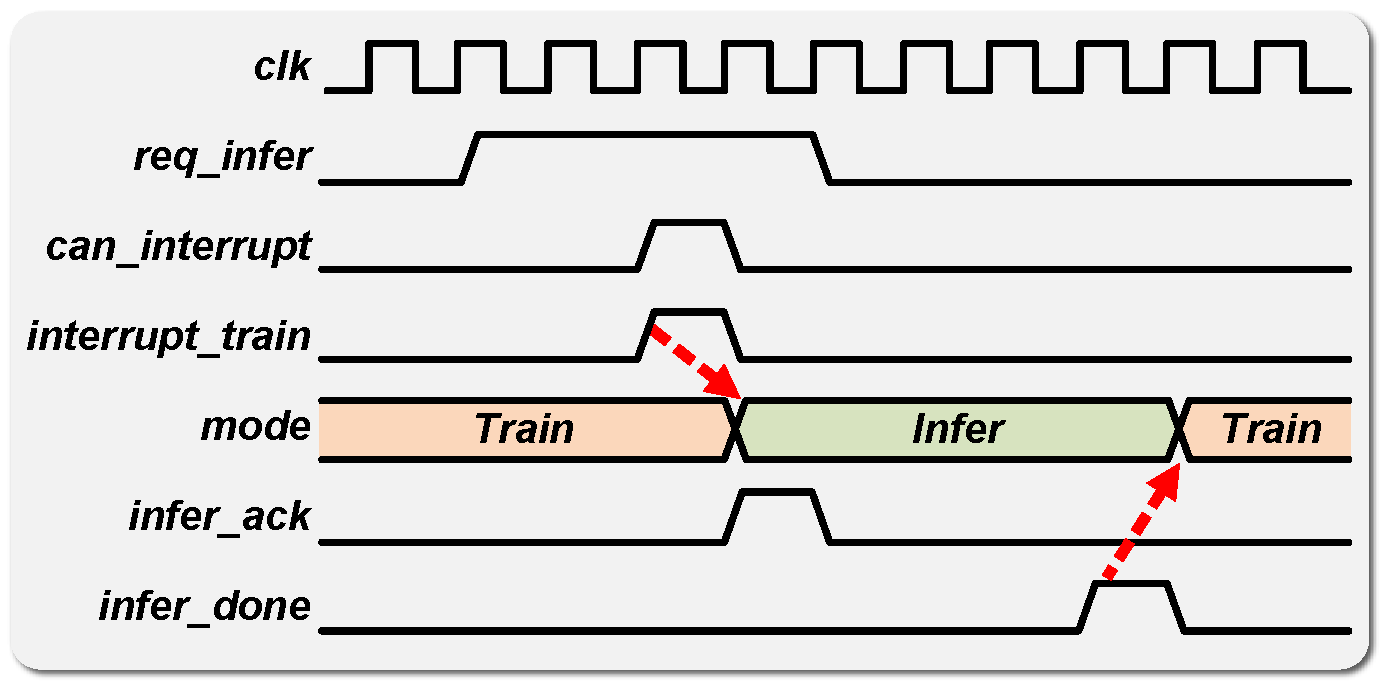
\includegraphics[width=0.9\linewidth]{Figures/Fig_IoR_waveform.pdf}\label{fig:ior_waveform}}

\caption{(a) Block diagram and (b) timing diagram of IMU.}\label{fig:IMU_total}
\vspace{-0.5cm}
\end{figure}


Fig. \ref{fig:IMU_total}\subref{fig:IMU} illustrates IMU, which is responsible for handling the proposed IoR scheduling scheme. IMU monitors training instructions and determines when they can be interrupted. To maximize on-chip data reuse, a training instruction can be interrupted only after all computations involving the on-chip data are complete and further reuse is not possible. When an inference request is received, IMU checks for interrupt availability and, if allowed, switches the processor to the inference mode. After the inference is completed, the processor returns to the training mode. Depending on the current mode, either the training or inference program counter is used to issue instructions. The operational timing diagram of IMU is shown in Fig. \ref{fig:IMU_total}\subref{fig:ior_waveform}.

Fig. \ref{fig:ior_comparison} shows the hardware utilization and required operating frequency for various inference-to-training ratios. When using conventional sequential scheduling, hardware utilization decreases as the inference-to-training ratio increases. In contrast, the proposed IoR scheduling maintains 100\% utilization across all inference-to-training ratios. This can be achieved since IoR scheduling performs training as a background task, while inference requests, which have higher priority, interrupt the ongoing training, eliminating idle periods caused by waiting for either phase to complete.

\begin{figure}[!t]
   \begin{center}
  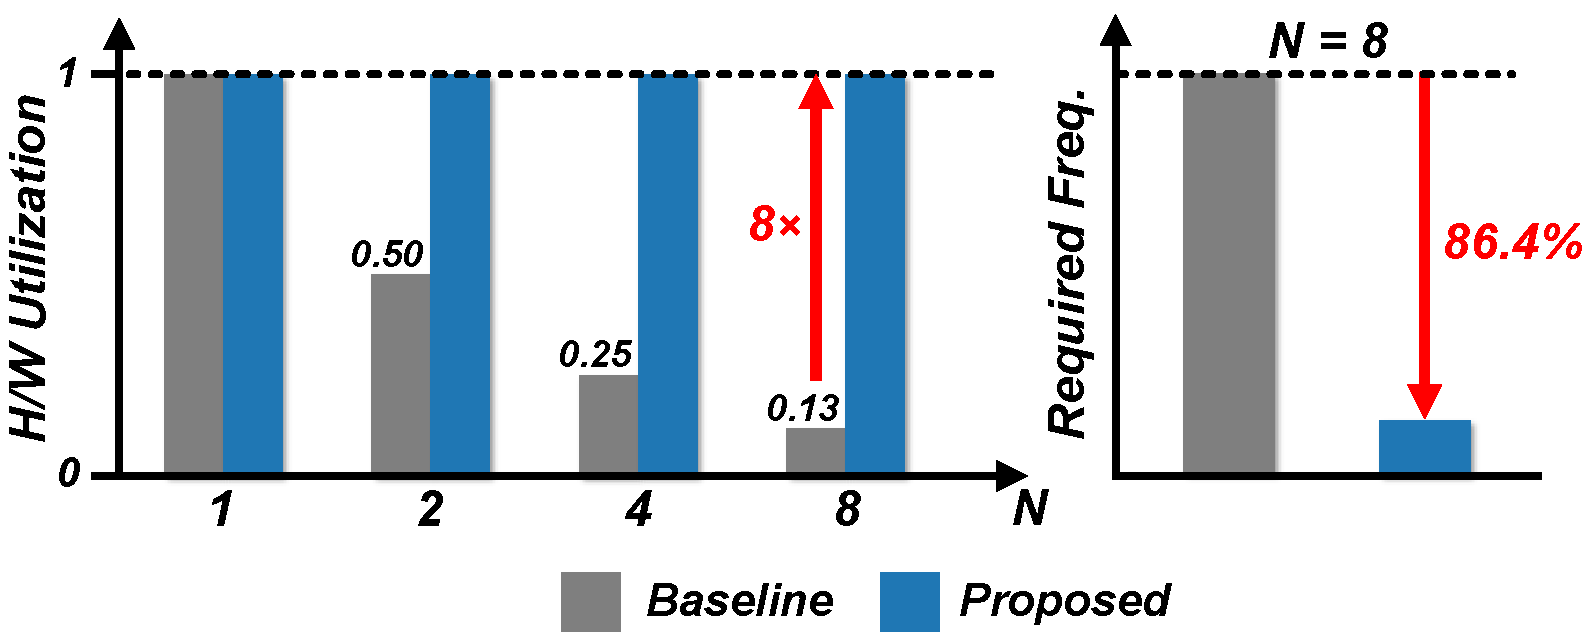
\includegraphics[width=0.95\linewidth]{Figures/Fig_IoR_comparison.pdf}\\
  \caption{Comparisons of hardware utilization and operation frequency.}\label{fig:ior_comparison}
   \end{center}
   \vspace{-0.5cm}
\end{figure}

Furthermore, at the optimal inference-to-training ratio of $N = 8$, the IoR scheduling reduces the required operating frequency to meet timing constraints by 86.4\% compared to conventional sequential scheduling, thereby significantly reducing processor power consumption. Simulation results also confirm that the worst-case inference latency remains within 10\% of the sensor input period under IoR scheduling, ensuring real-time response and stable navigation performance.

\subsection{Adaptive Dataflow Mapping}


\begin{figure*}[!t]
% \centering
\begin{center}

\subfloat[]{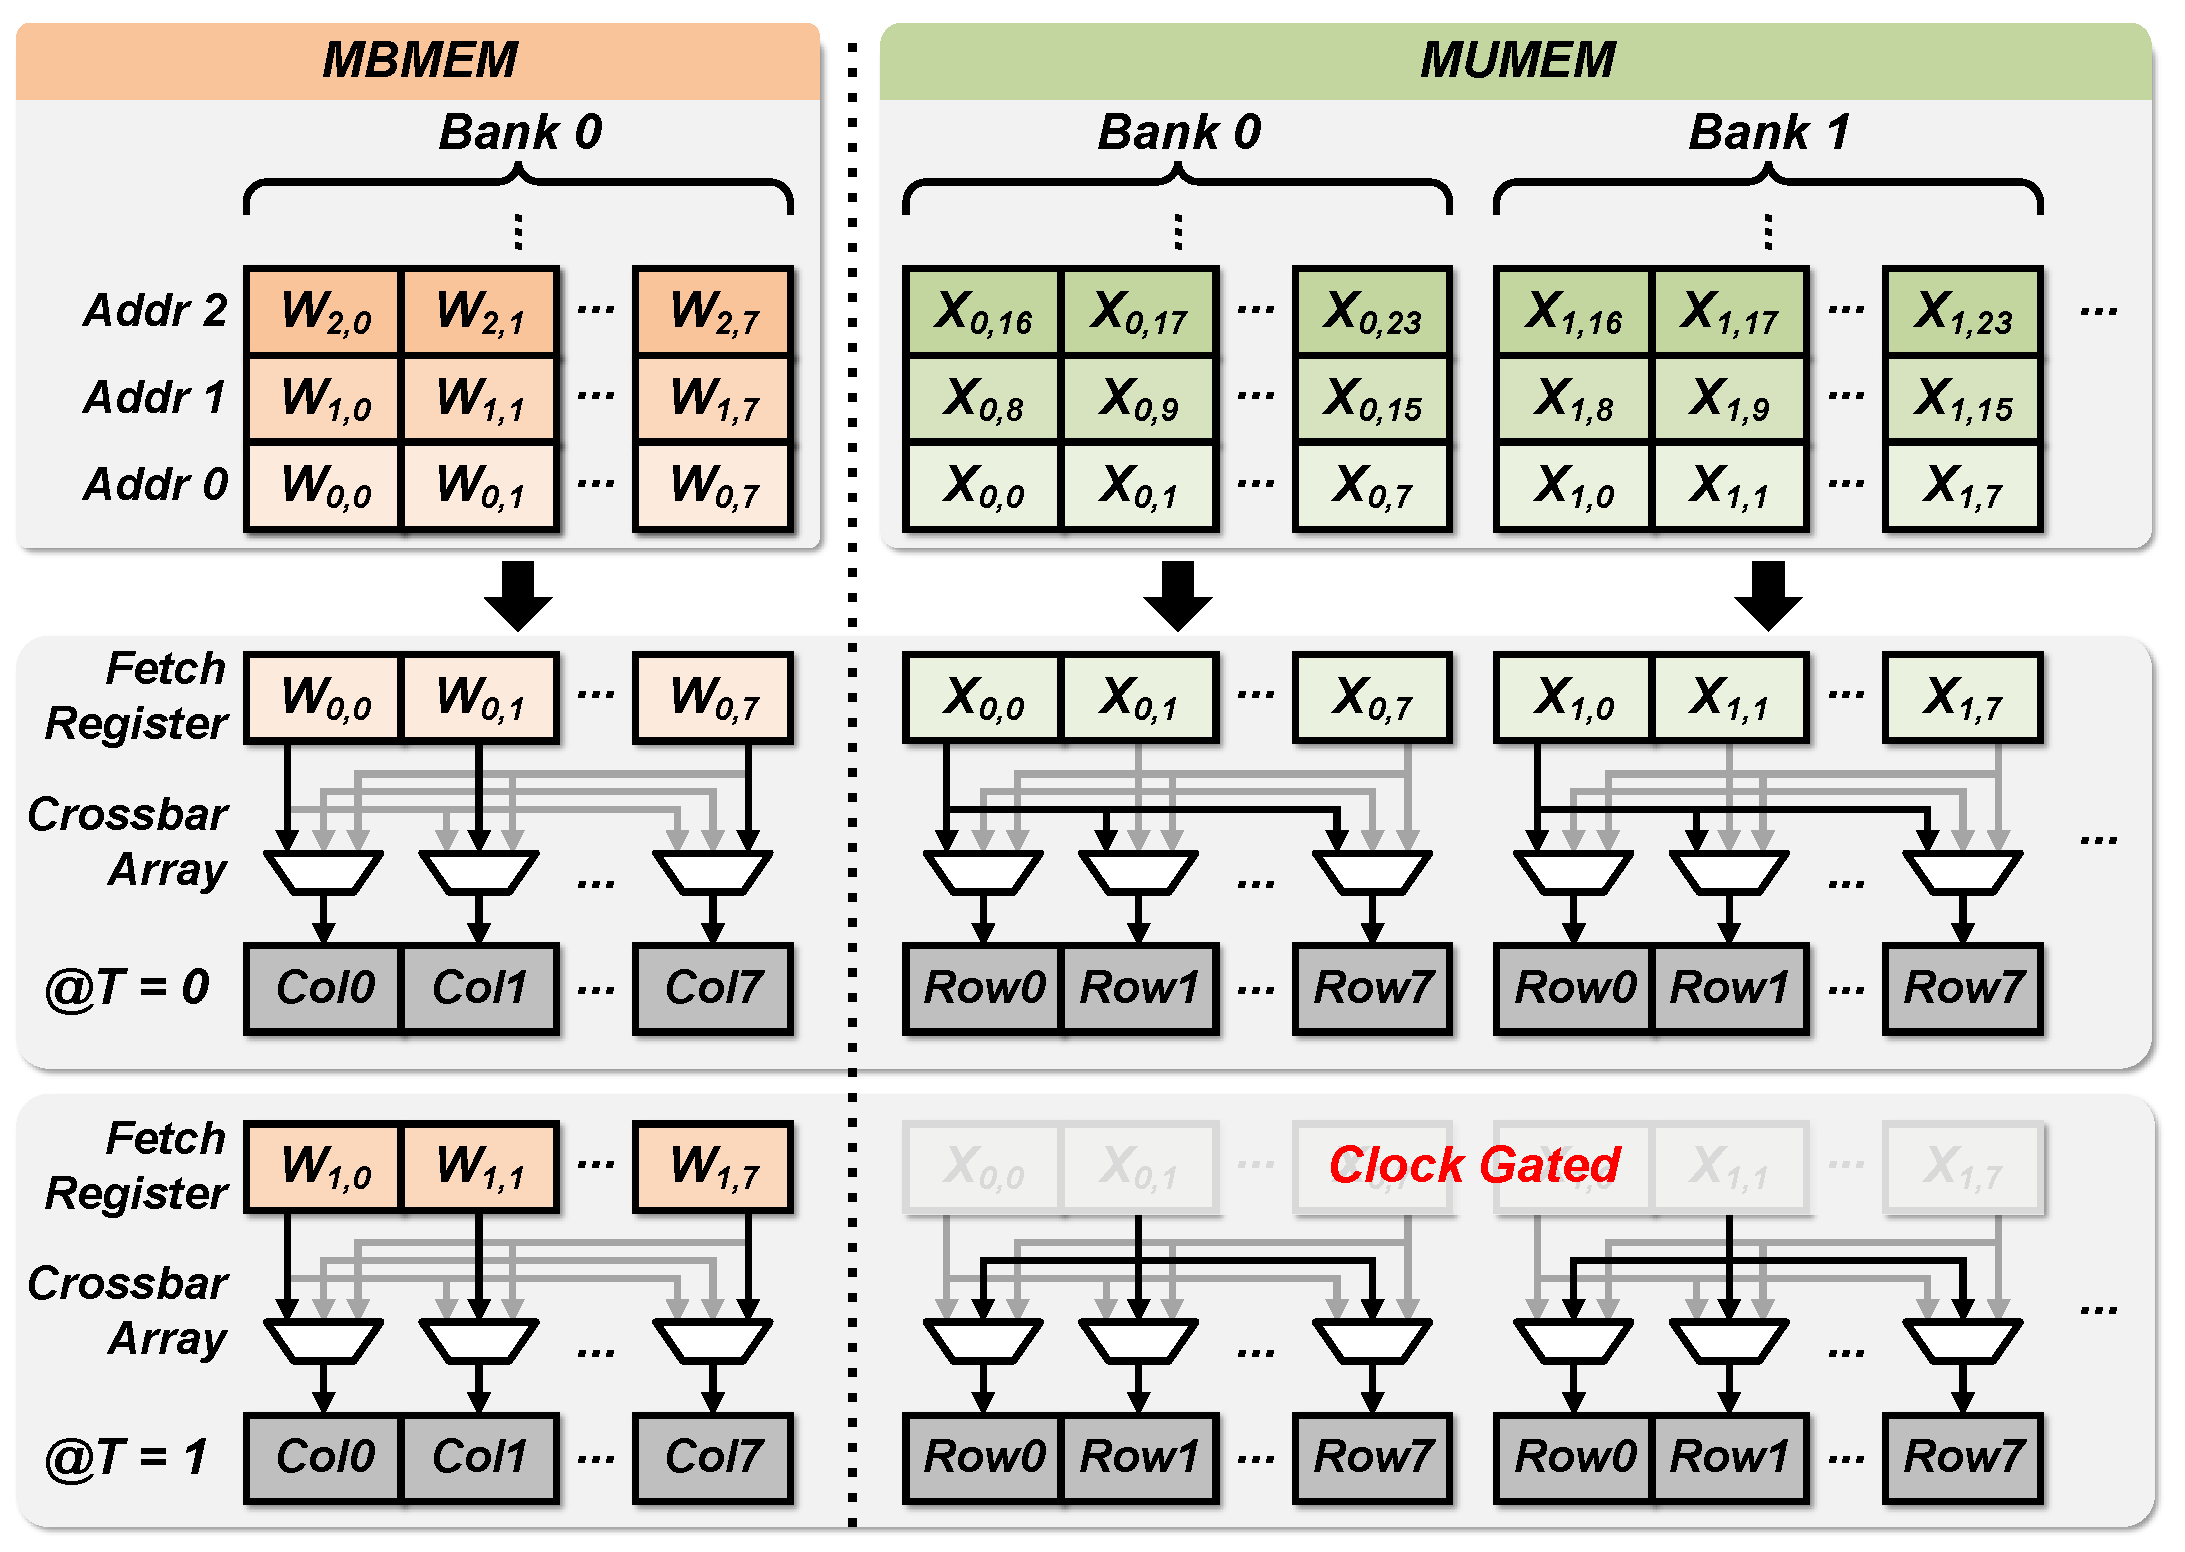
\includegraphics[width=.45\linewidth]{Figures/Fig_dataflow_multibatch_rev1_cropped.pdf}\label{fig:dataflow_training}}
\hspace{2.5mm}
\subfloat[]{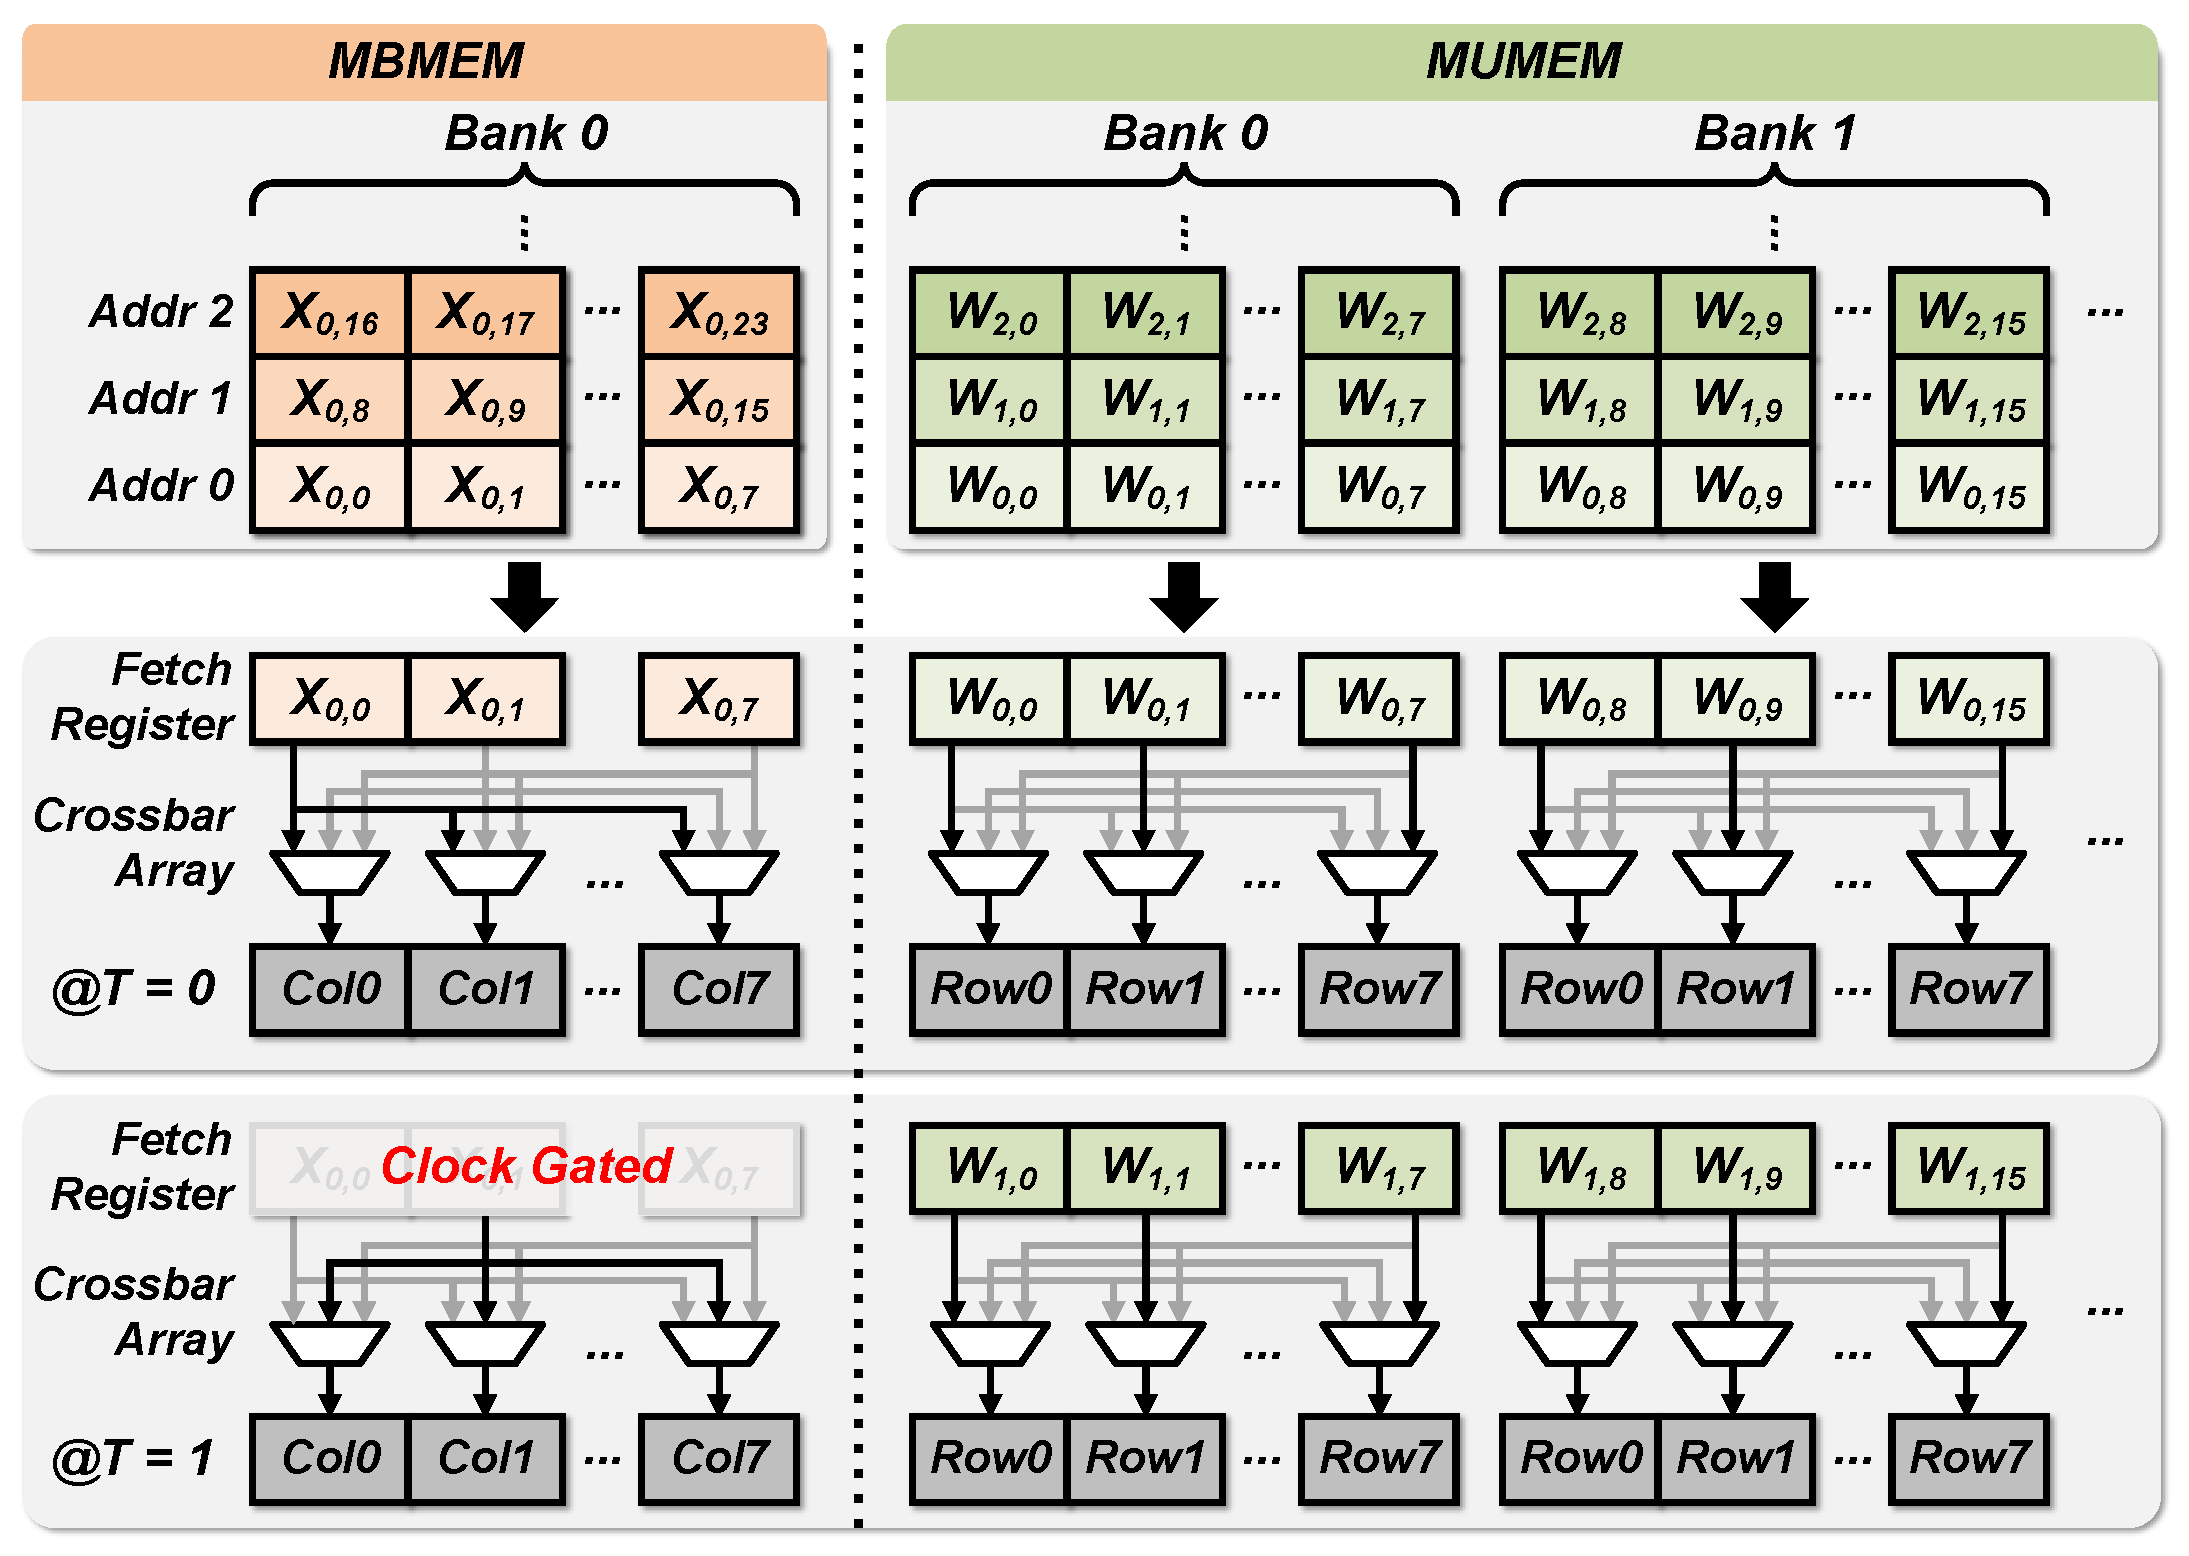
\includegraphics[width=.45\linewidth]{Figures/Fig_dataflow_singlebatch_rev1_cropped.pdf}\label{fig:dataflow_inference}}

\subfloat[]{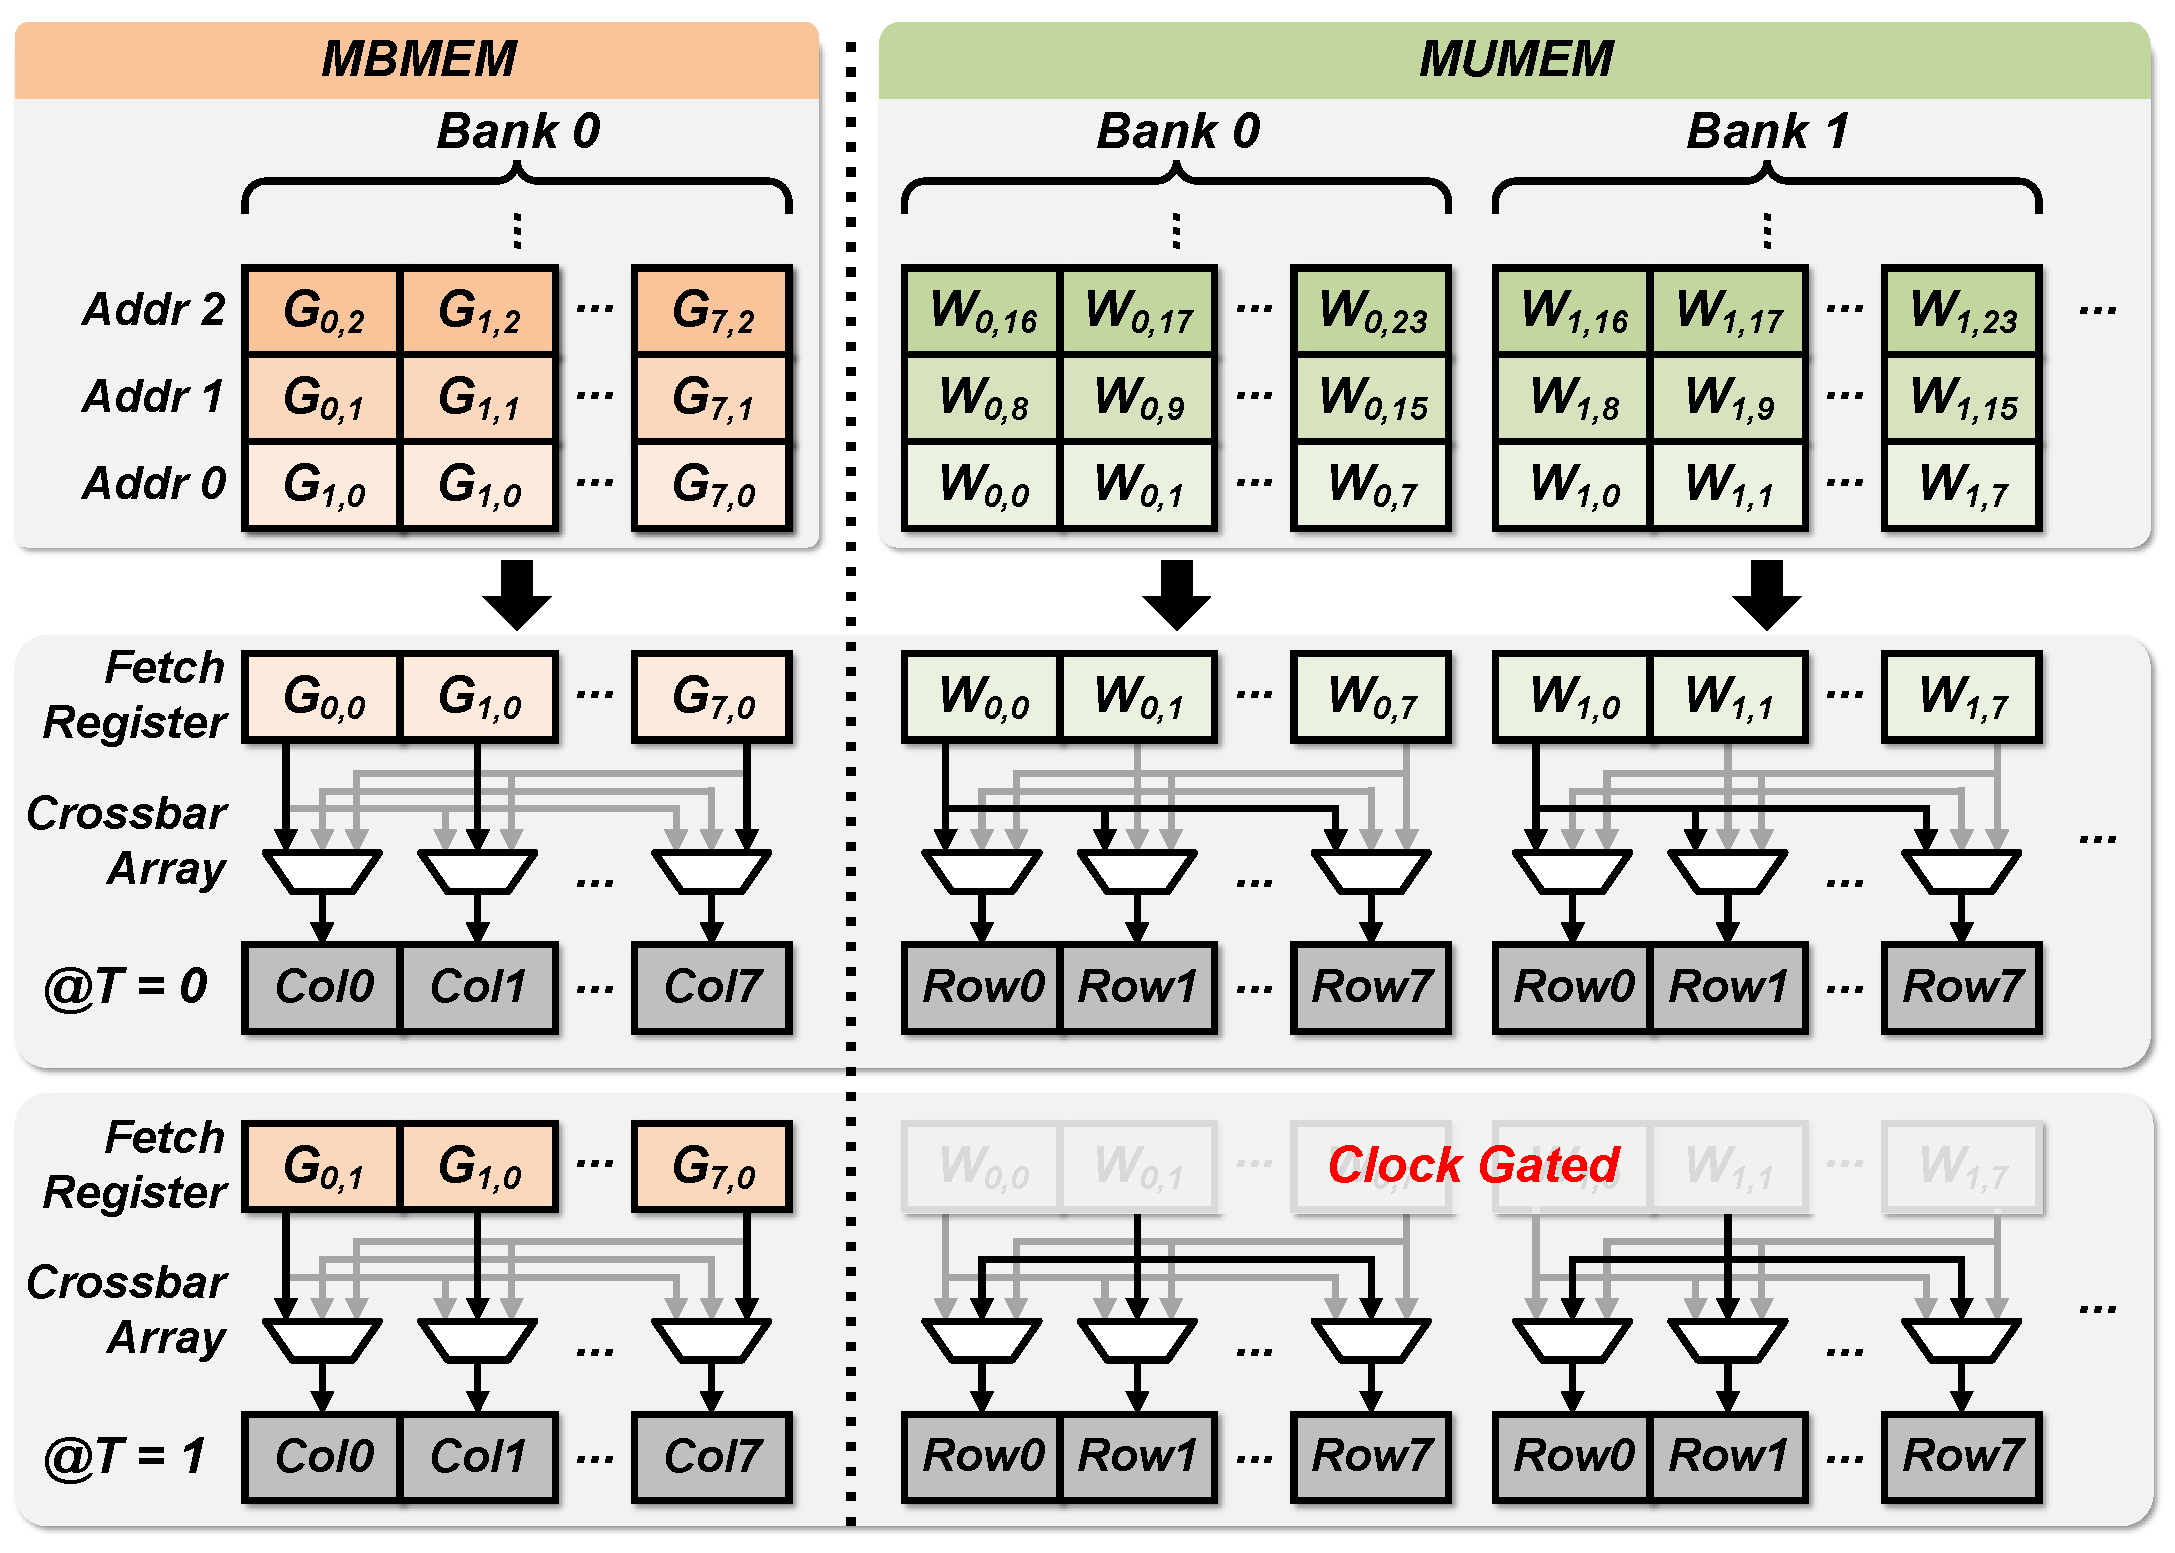
\includegraphics[width=.45\linewidth]{Figures/Fig_dataflow_dX_rev1_cropped.pdf}\label{fig:dataflow_dx}}
\hspace{2.5mm}
\subfloat[]{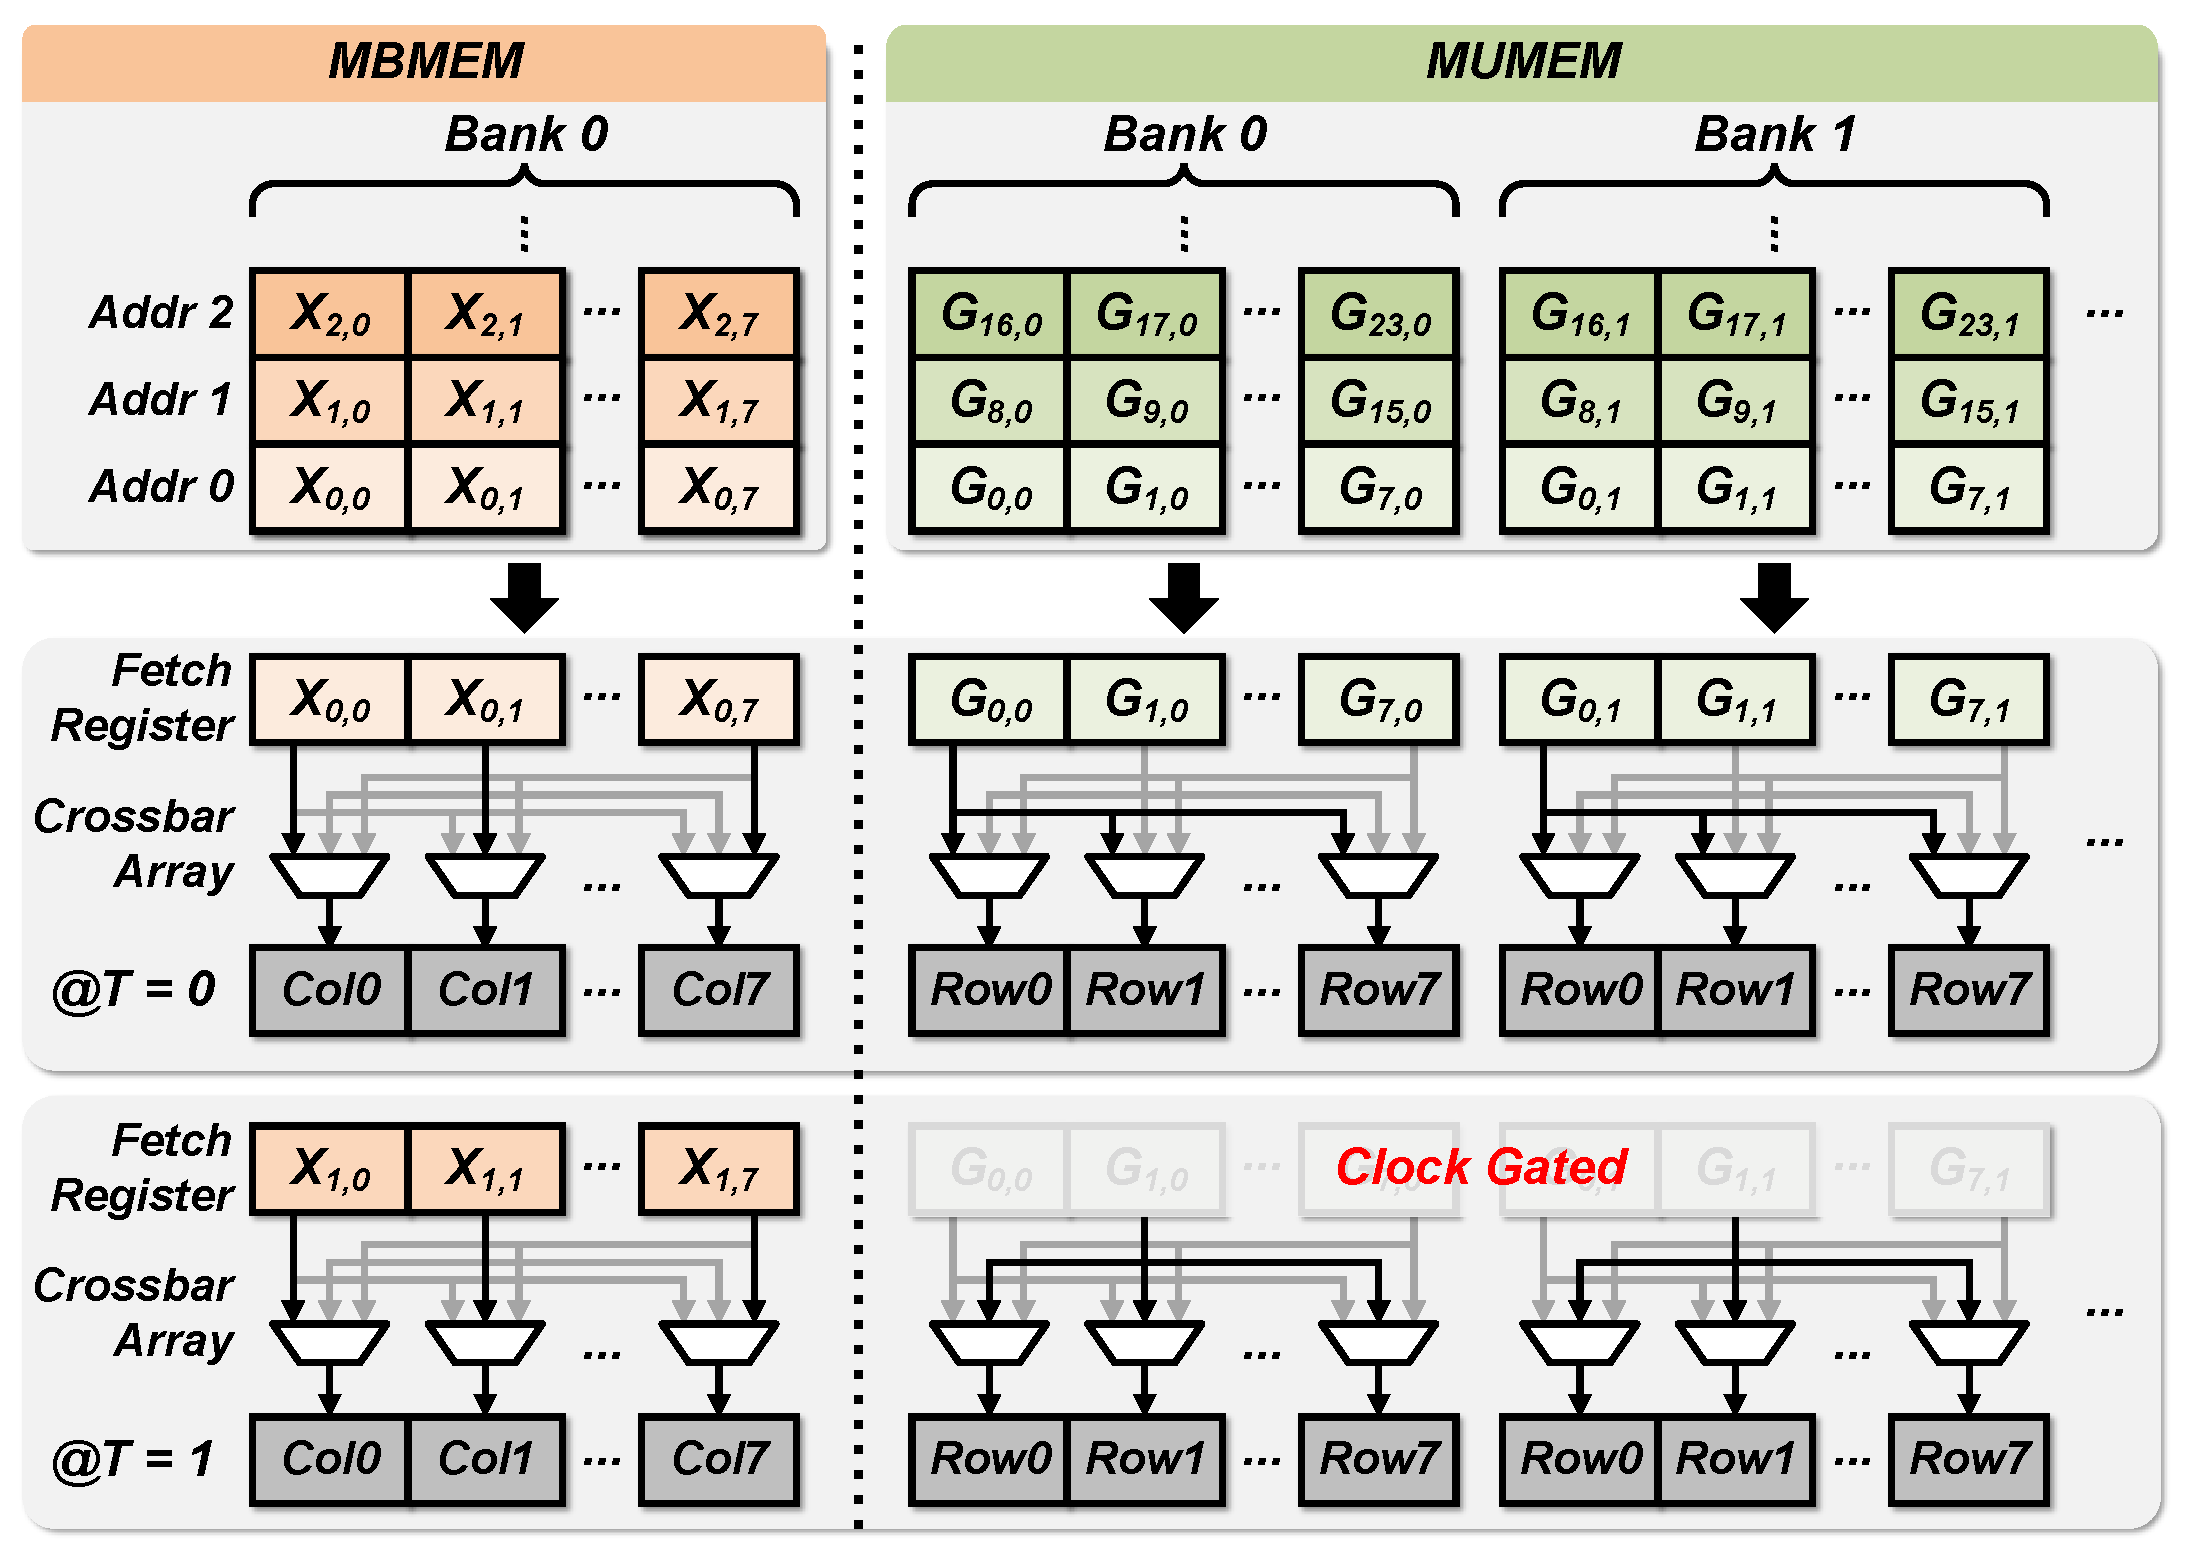
\includegraphics[width=.45\linewidth]{Figures/Fig_dataflow_dW_rev1_cropped.pdf}\label{fig:dataflow_dw}}

% \vspace{-0cm}

\caption{Dataflow for (a) multi-batch feed-forward, (b) single-batch feed-forward, (c) activation gradient computation, and (d) weight gradient computation.}\label{fig:dataflow}
\end{center}
\vspace{-0.7cm}
\end{figure*}

DRL training requires both single-batch and multi-batch feed-forward execution. Therefore, our processor is designed to efficiently support both single-batch and multi-batch feed-forward operations by adaptively reconfiguring the dataflow according to the workload. The dataflow is dynamically switched, while MBMEM and MUMEM are flexibly utilized to maintain high PE array utilization. For both activation and weight gradient computation, weights, activations, and activation gradients required for the computation are stored in DRAM as groups of eight contiguous elements. To exploit these 8-way groups without fragmentation, we allocate the data differently in MBMEM and MUMEM for activation-gradient and weight-gradient updates, respectively, allowing each kernel to consume fully packed bursts and sustain high compute and bandwidth efficiency.


In a prior RL processor in \cite{ISSCC19}, the data in the row buffer is broadcast only along PE rows, which at the array level implements multicasting. When the input batch size is small, input features are unicast across the PE array, with the batch dimension mapped to the array width; this mapping severely reduces PE utilization in the single-batch feed-forward operations (batch size = 1). In contrast, our design further optimizes the dataflow so that, even under single-batch feed-forward, the input feature is broadcast across the entire PE array rather than row-limited multicast, enabling full-array usage and mitigating batch-size dependences.

MBMEM is implemented as a single bank and is connected to the PE array in a row-wise manner, allowing each PE in a row to receive identical data. It can operate in broadcast mode, delivering identical data to all rows, or in multicast mode, delivering distinct data per row. In contrast, MUMEM comprises 32 banks connected in a column-wise manner to the PE array, with each bank mapped to a PE column. MUMEM can operate in multicast mode, sending the same data to each row, or in unicast mode, providing unique data to each row.

Fig. \ref{fig:dataflow} illustrates the data distribution strategies of MBMEM and MUMEM for different operational modes. Data distribution is adaptively reconfigured by nine crossbar arrays at the output of MBMEM and MUMEM, incurring only 0.35\% area overhead. Each crossbar array consists of eight 8:1 multiplexers. For multi-batch feed-forward used in training (Fig. \ref{fig:dataflow}\subref{fig:dataflow_training}), weights and activations are stored in MBMEM and MUMEM, respectively, both utilizing input-channel-first addressing, such that the memory address increases with the input channel index. In MUMEM, the output-channel indices of activations are mapped to bank indices. Each memory read is buffered in fetch registers, where each bank has 128-bit width accommodating eight 16-bit values. The weights stored in MBMEM are multicasted to all columns via the crossbar, while the activations stored in MUMEM are multicasted to all rows for each column. The fetch registers retain loaded data for eight cycles with only routing adjustments, and clock-gating is applied to minimize power consumption.

For single-batch feed-forward used in inference (Fig. \ref{fig:dataflow}\subref{fig:dataflow_inference}), the allocation of activations and weights is reversed; activations and weights are stored in MBMEM and MUMEM, respectively. However, the addressing scheme remains input-channel-first, as in the training mode. The output channel indices of weights increase with the MUMEM bank index. MBMEM broadcasts the activations to all columns, enabling each fetch register to supply data for eight cycles through routing adjustments, with clock-gating for energy efficiency. In contrast, MUMEM unicasts the weights to each PE. This adaptive dataflow mapping scheme across training and inference enables high memory utilization and minimizes both latency and power overhead.


The proposed mapping further supports weight gradient and activation gradient computation during backpropagation without requiring an additional transposer. For activation gradient computation (Fig. \ref{fig:dataflow}\subref{fig:dataflow_dx}), output gradients and weights are stored in MBMEM and MUMEM, respectively, both using output-channel-first addressing (i.e., memory addresses increase with the output channel index), and in MUMEM, input channel indices of weights are mapped to bank indices. For weight gradient computation (Fig. \ref{fig:dataflow}\subref{fig:dataflow_dw}), activations and output gradients are stored in MBMEM and MUMEM, respectively, both using batch-first addressing, where memory addresses increase with the batch index, and in MUMEM, output channel indices of gradients are mapped to bank indices. The data distribution scheme for MBMEM and MUMEM is identical to that used for activation gradient calculation.

\begin{figure}[!t]
   \begin{center}
  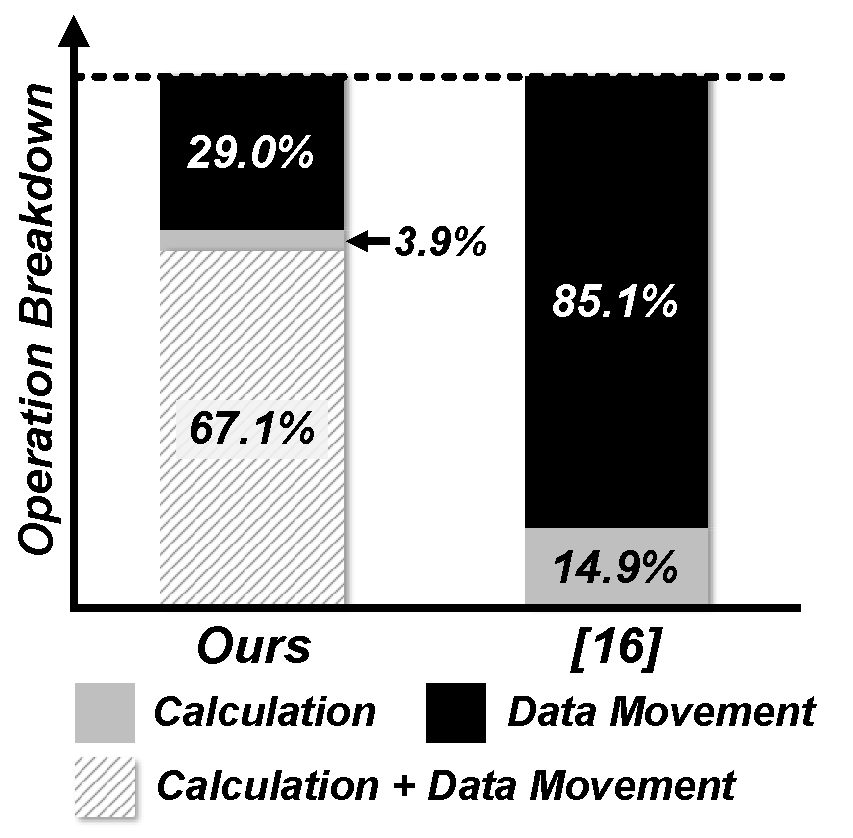
\includegraphics[width=0.6\linewidth]{Figures/Fig_pe_utilization_rev1_v2_cropped.pdf}\\
  \caption{Operation breakdown comparison.}\label{fig:pe_utilization}
   \end{center}
   \vspace{-0.5cm}
\end{figure}

By adopting this adaptive dataflow mapping, the processor efficiently supports all of multi-/single-batch feed-forward, and weight/activation gradient calculations. Furthermore, by closely matching the arithmetic intensity of the algorithm and hardware, the design achieves a high PE array utilization of 71.0\% including external I/O latency throughout the training scenario, significantly outperforming a prior design in \cite{VLSI21}, as shown in Fig. \ref{fig:pe_utilization}.


\subsection{Column-wise Zero-Skipping Categorical Projection}

While conventional DRL algorithms often represent Q-values as scalars, this can fail to capture the uncertainty in value estimation, which is critical in safety-sensitive domains such as autonomous navigation \cite{ur23}. DistRL algorithms model Q-values as probability distributions (Q-distributions), thereby capturing the full range of possible outcomes and providing a richer training signal \cite{C51}. In particular, C51 \cite{C51} demonstrated that directly approximating the return distribution can improve the stability and performance of DRL algorithms under function approximation and non-stationary policies. By explicitly modeling the value distribution, DistRL methods yield superior empirical results in complex tasks such as Atari games. By quantifying uncertainty, this approach enables more robust and reliable policy learning in dynamic and uncertain environments.

\begin{figure}[!t]
   \begin{center}
  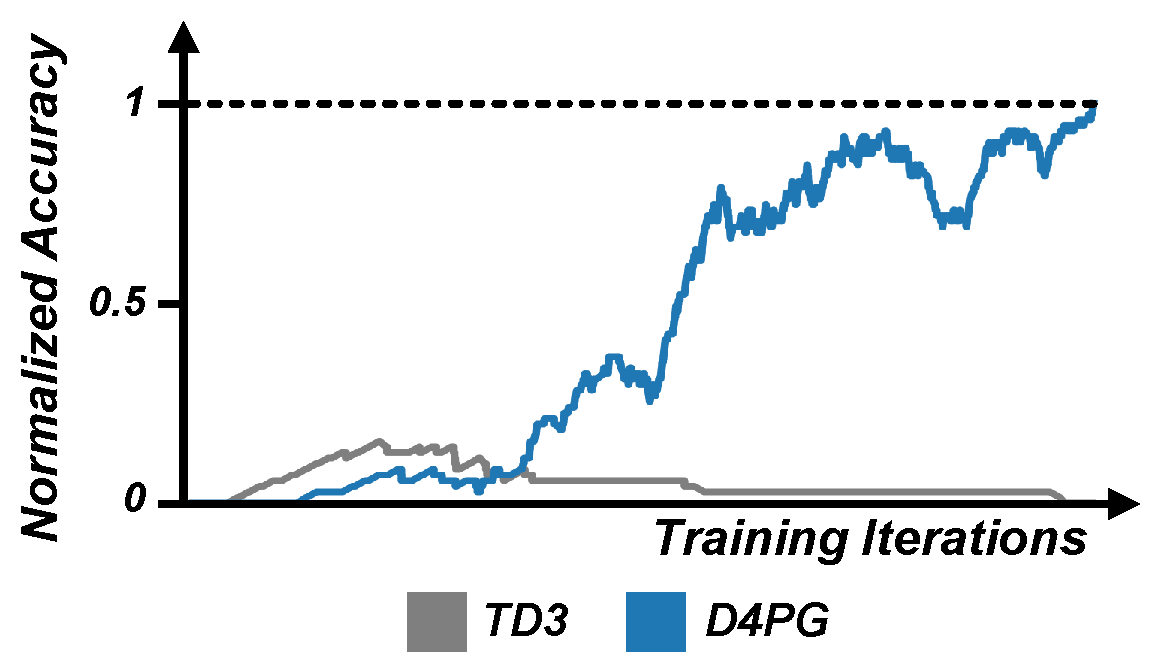
\includegraphics[width=0.83\linewidth]{Figures/Fig_td3_vs_d4pg.pdf}\\
  \caption{Training performance comparisons between TD3 and D4PG.}\label{fig:td3_vs_d4pg}
   \end{center}
   \vspace{-0.8cm}
\end{figure}


Recent works in mapless navigation have further demonstrated the practical benefits of DistRL. In particular, previous studies \cite{NCTU, nctu_fr} report that D4PG, a DistRL algorithm, achieves improved performance and robustness compared to conventional value-based methods in real-world navigation tasks. Furthermore, a recent theoretical and empirical analysis revealed that the advantages of DistRL become particularly significant when combined with deep neural network function approximation, rather than in simple tabular or linear settings \cite{AAAI19}. To further validate these findings, we experimentally compared D4PG, which is a DistRL algorithm, and TD3, a conventional scalar Q-value-based DRL algorithm, on a real-world autonomous navigation task. As demonstrated in Fig. \ref{fig:td3_vs_d4pg}, D4PG successfully learns a high-performance navigation policy and exhibits stable convergence throughout training. In contrast, TD3, a conventional scalar Q-value-based DRL algorithm, fails to learn a successful policy in this scenario. These results empirically confirm that DistRL enables effective policy learning in practical autonomous navigation tasks, where conventional scalar Q-value-based methods may struggle to converge.

\begin{figure}[!t]
   \begin{center}
  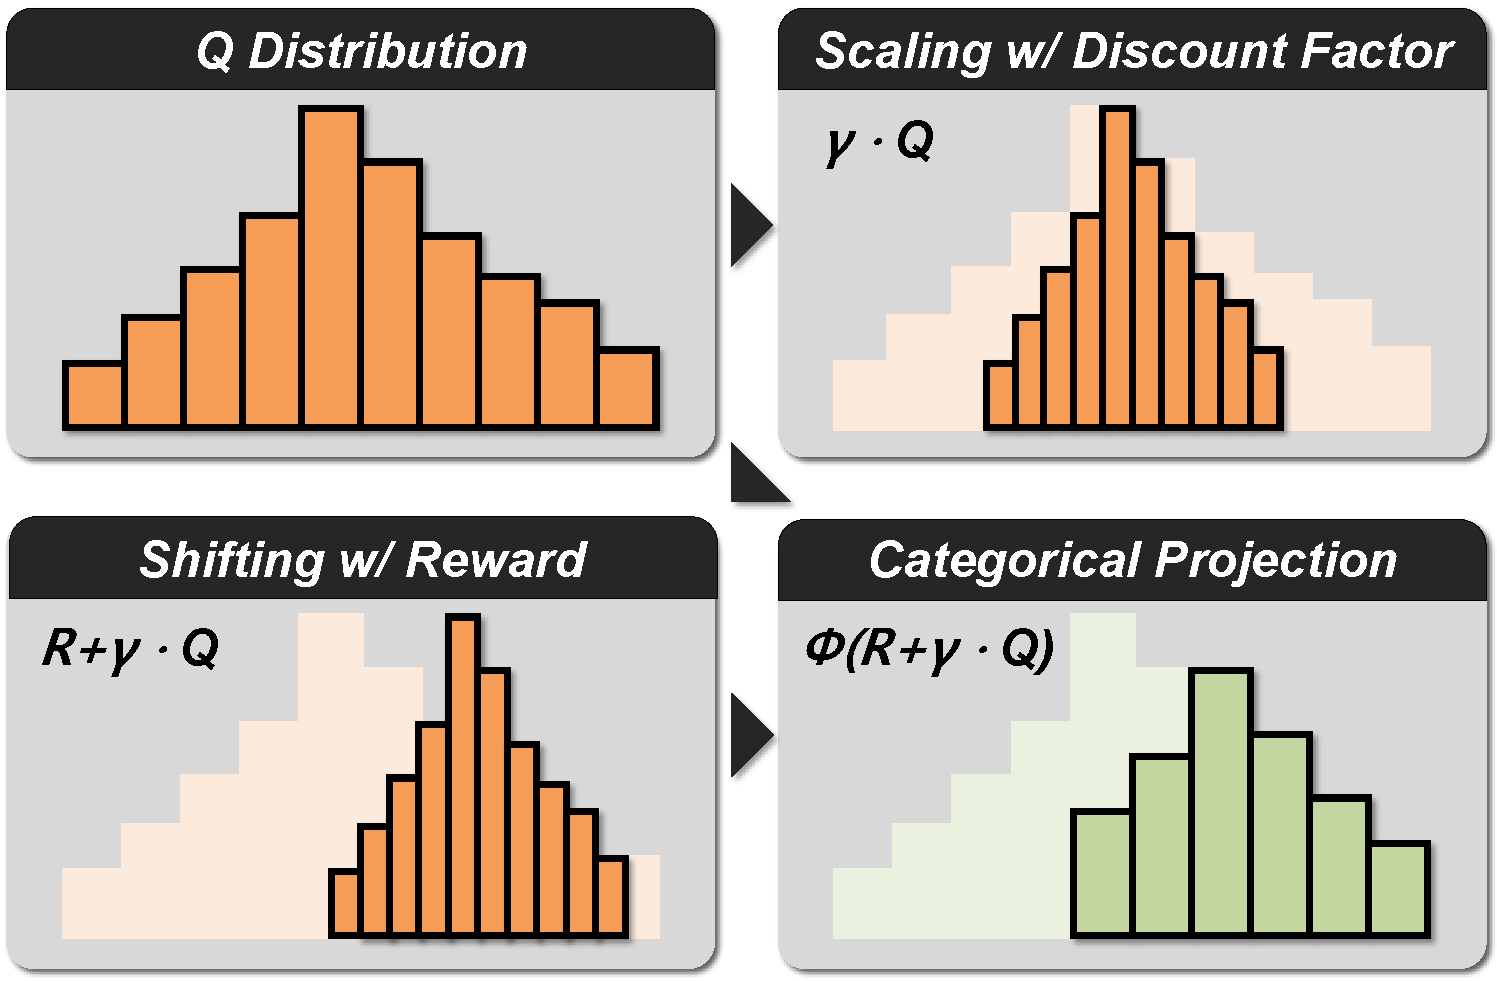
\includegraphics[width=0.9\linewidth]{Figures/Fig_projection_overview.pdf}\\
  \caption{Overview of categorical projection.}\label{fig:projection_overview}
   \end{center}
   \vspace{-0.5cm}
\end{figure}

Fig. \ref{fig:projection_overview} illustrates the motivation for categorical projection in DistRL algorithms. Unlike conventional RL algorithms that represent the Q-value as scalar, DistRL models the entire distribution of Q-values (Q-distribution). During training, the target Q-distribution undergoes a linear transformation by the reward ($R$) and the discount factor ($\gamma$). As a result, the transformed target distribution is generally misaligned with the fixed support of the original Q-distribution. Therefore, to compute the loss, it is necessary to redistribute the transformed target distribution onto the original fixed support, a process known as categorical projection \cite{C51}. This projection ensures that the distributional Bellman target and the network output are represented on the same discrete support, enabling a consistent and well-defined loss computation.

\begin{figure}[!t]
\centering

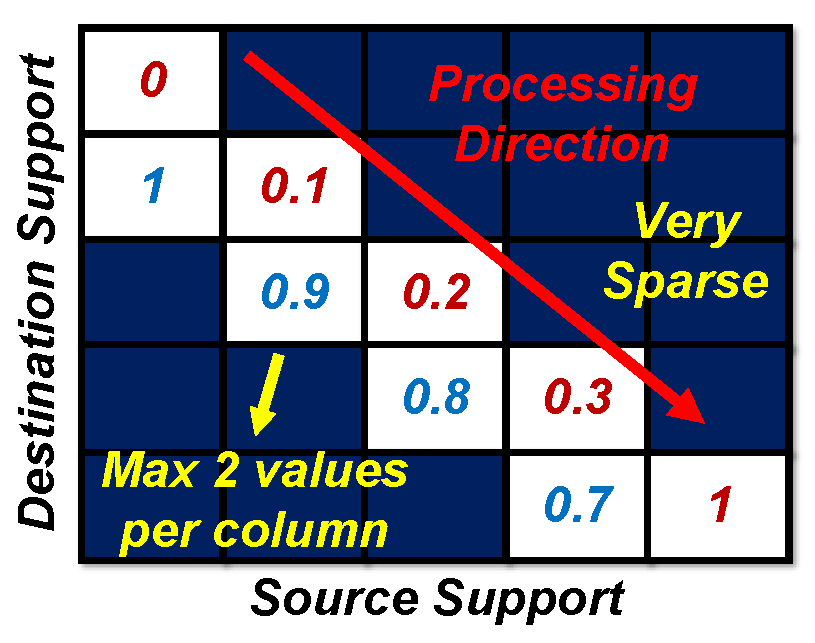
\includegraphics[width=0.6\linewidth]{Figures/Fig_delta_h_matrix.pdf}

\caption{An example of $\Delta h$ matrix with 5 supports.} \label{fig:delta_h_matrix}
\vspace{-0.5cm}
\end{figure}


Fig. \ref{fig:delta_h_matrix} illustrates the $\Delta h$ matrix utilized in categorical projection. This matrix encodes the redistribution of probability from each source support to the corresponding destination supports. Since the probability from each source support can be assigned to at most two neighboring destination supports, the $\Delta h$ matrix is inherently sparse, containing at most two non-zero entries per column. Consequently, the matrix exhibits high sparsity, reaching up to 96.1\% for 51 supports. To exploit this sparsity, our design employs column-wise zero-skipping categorical projection scheme. This scheme fetches and processes only the non-zero elements in each column per cycle, thereby skipping unnecessary operations for zero values in the $\Delta h$ matrix and reducing both computation overhead and power consumption. As a result, the proposed projection scheme reduces the total number of projection operations by 99\% for 51 supports.

\begin{figure}[!t]
\centering

\subfloat[]{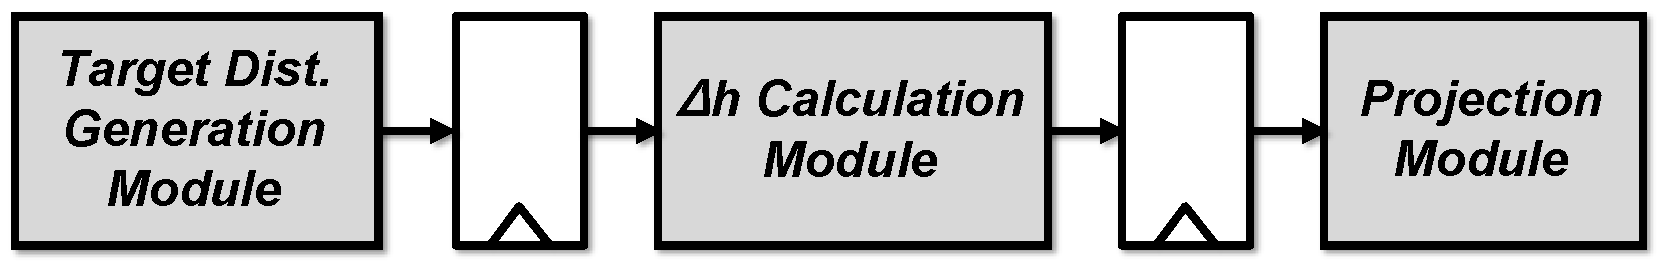
\includegraphics[width=0.95\linewidth]{Figures/Fig_ppu.pdf}\label{fig:ppu}}

\subfloat[]{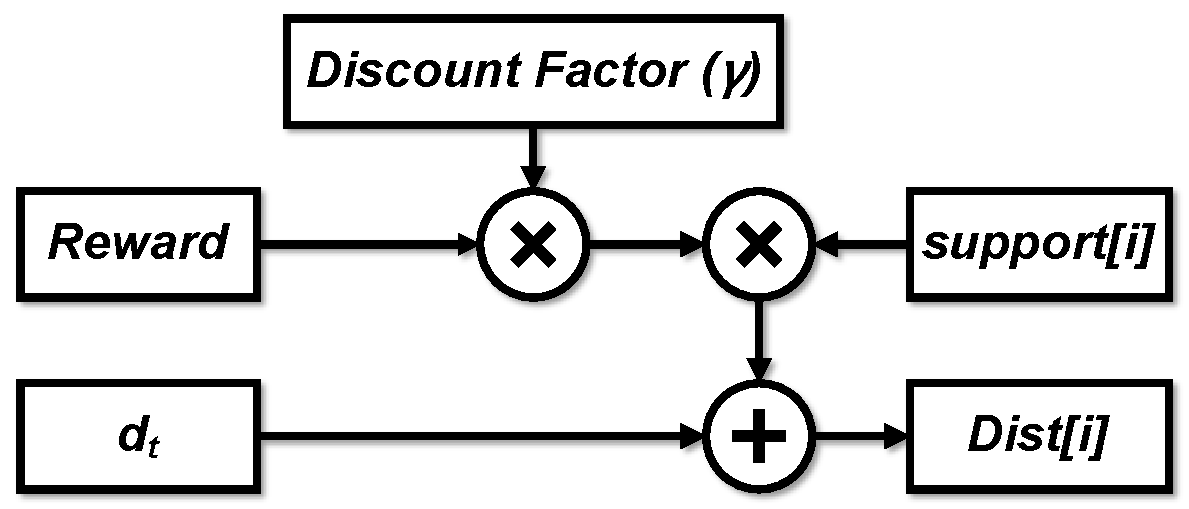
\includegraphics[width=0.7\linewidth]{Figures/Fig_target_dist_gen_module.pdf}\label{fig:target_dist_gen_module}}

\subfloat[]{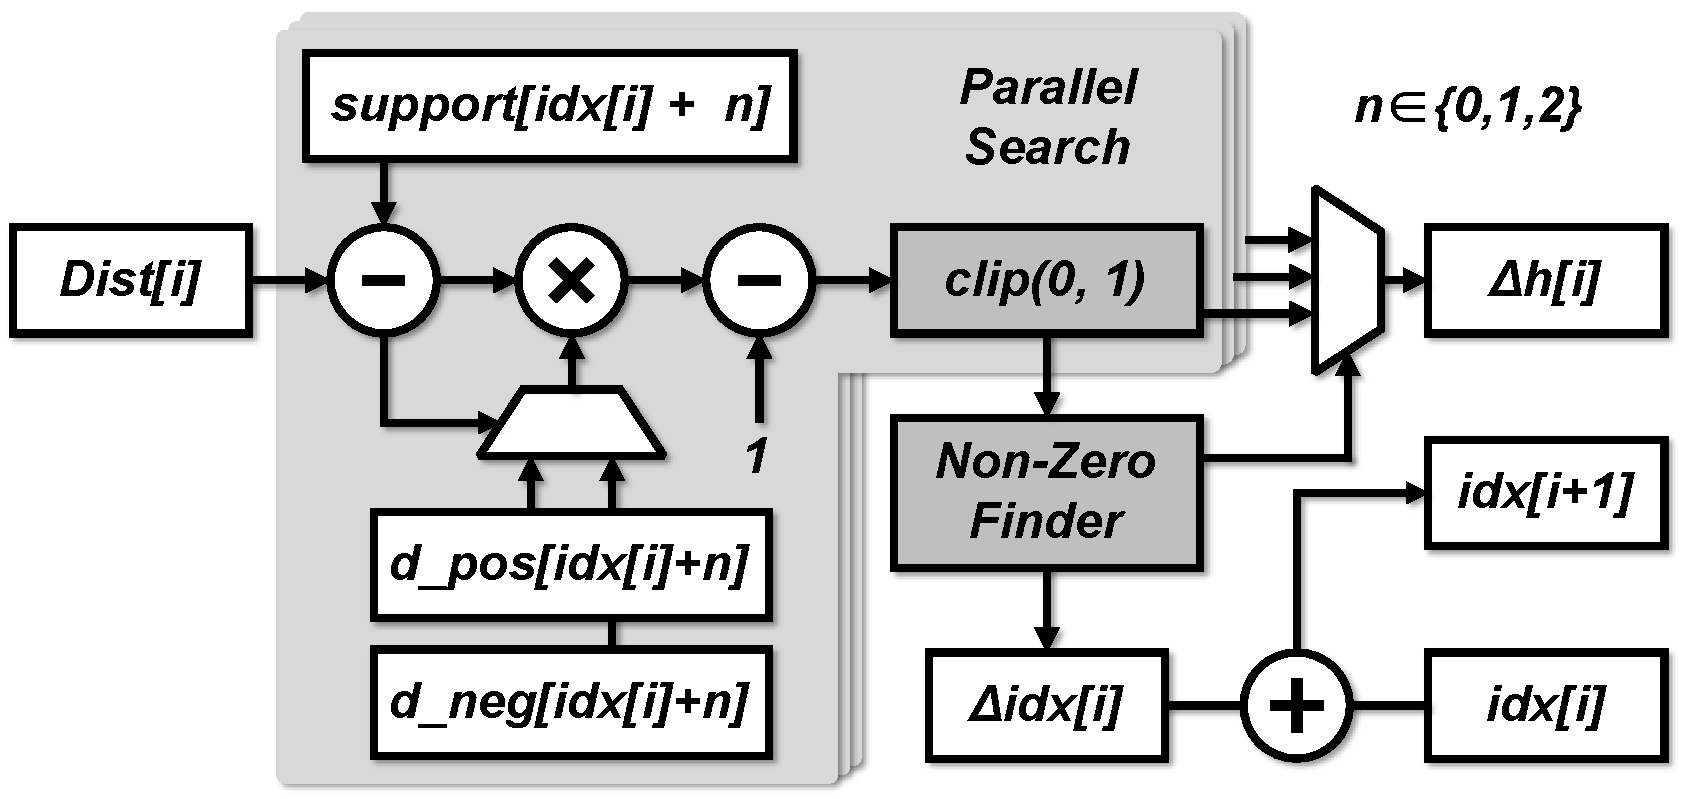
\includegraphics[width=0.95\linewidth]{Figures/Fig_delta_h_module.pdf}\label{fig:delta_h_module}}

\subfloat[]{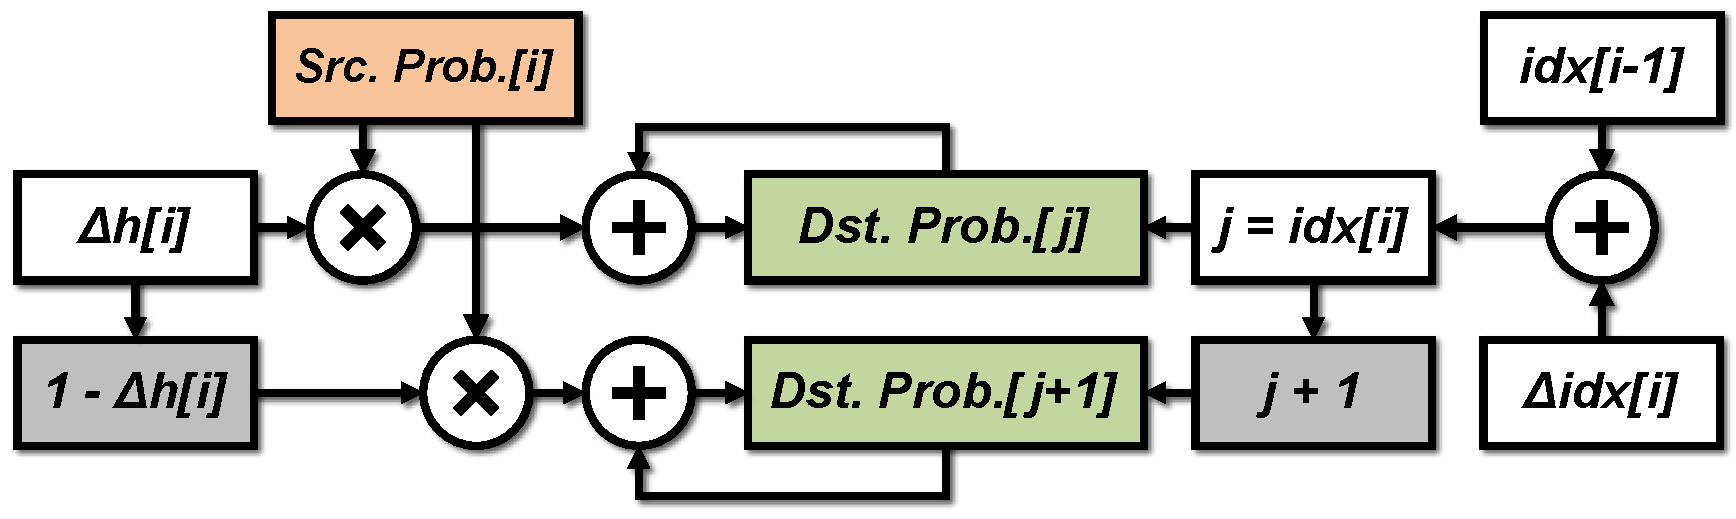
\includegraphics[width=0.95\linewidth]{Figures/Fig_projection_module.pdf}\label{fig:projection_module}}

\caption{(a) Projection Processing Unit (PPU). (b) Target distribution generation module. (c) $\Delta h$ calculation module. (d) Projection module. }\label{fig:ppu_top}
\vspace{-0.5cm}
\end{figure}

The PPU block in our processor handles the proposed column-wise zero-skipping categorical projection. Fig. \ref{fig:ppu_top}\subref{fig:ppu} shows the overall architecture of PPU, which consists of a target distribution generation module, a $\Delta h$ calculation module, and a projection module. The target distribution generation module (Fig. \ref{fig:ppu_top}\subref{fig:target_dist_gen_module}) applies an affine transformation to the original Q-distribution using the discount factor ($\gamma$) and reward ($R$). The $\Delta h$ calculation module (Fig. \ref{fig:ppu_top}\subref{fig:delta_h_module}) computes the $\Delta h$ matrix. Rather than calculating the entire $\Delta h$ matrix, this module tracks the row indices of non-zero elements ($\text{idx}$) in each column. The difference between two adjacent indices, $\Delta \text{idx}$, can take only one of three possible values, ${0, 1, 2}$, based on our simulation using discount factor $\gamma=0.99$. Accordingly, the module computes the $\Delta h$ values for three candidate positions in parallel. A non-zero finder then detects the next non-zero row index ($\text{idx}$) for each column. Finally, the projection module (Fig. \ref{fig:ppu_top}\subref{fig:projection_module}) accumulates the redistributed source probabilities into the corresponding destination support bins.

\begin{figure}[!t]
\begin{center}
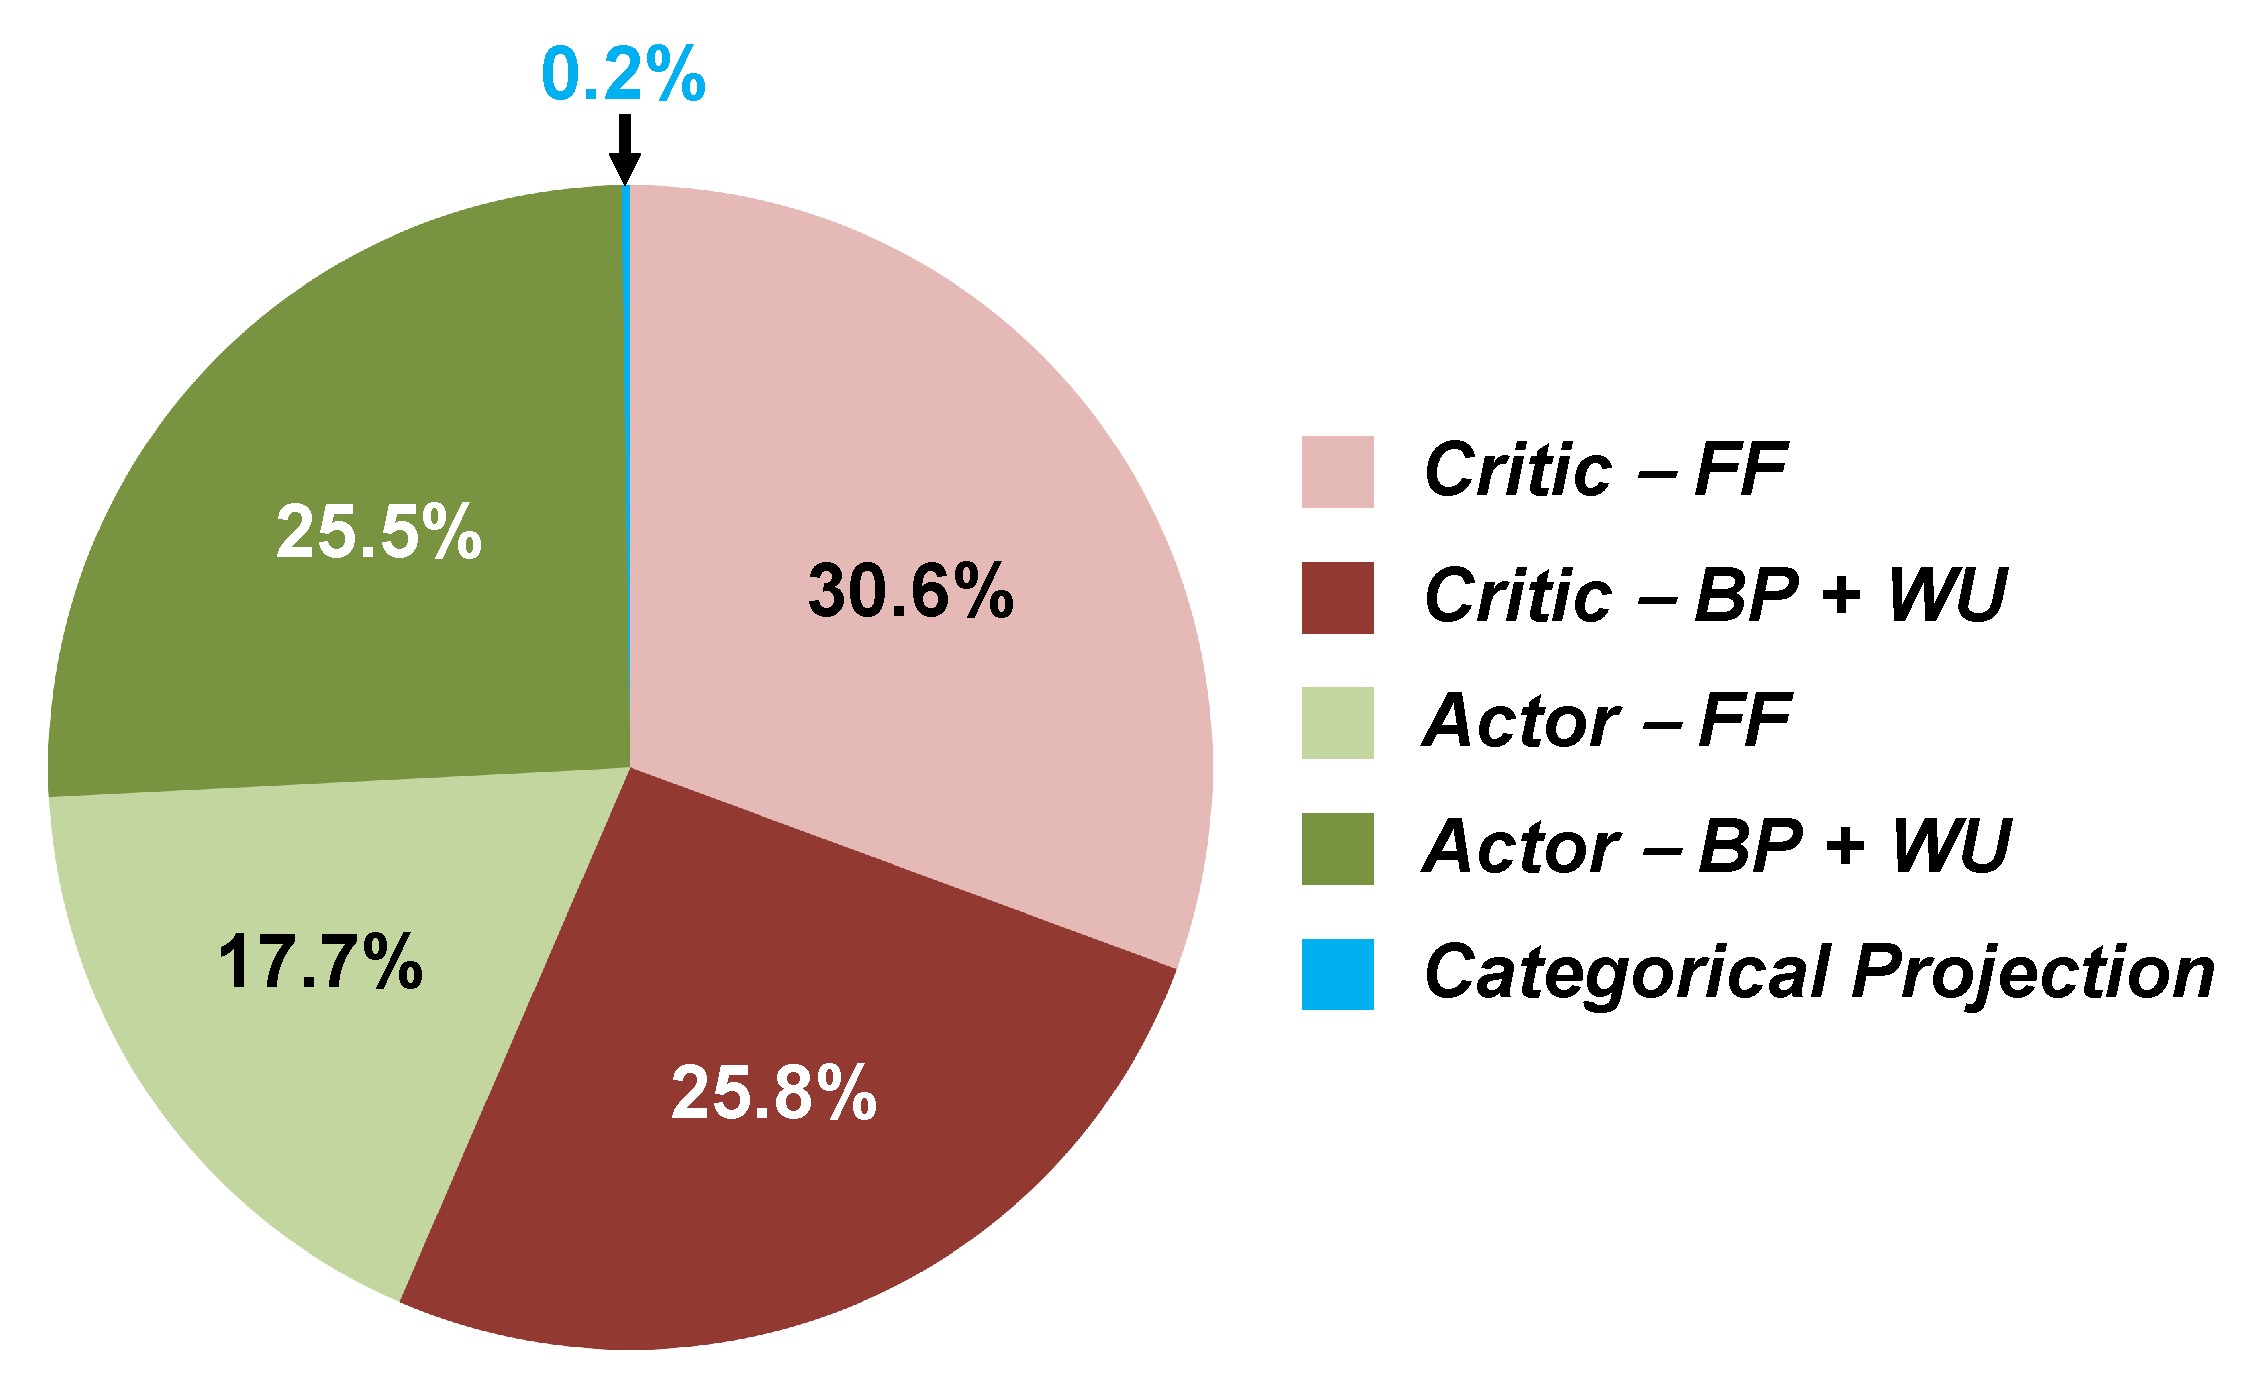
\includegraphics[width=0.85\linewidth]{Figures/Fig_training_ops_breakdown_rev1_v3_cropped.pdf}\\
\caption{Training operations breakdown.}\label{fig:training_ops_breakdown}
\end{center}
\vspace{-0.3cm}
\end{figure}

Fig. \ref{fig:training_ops_breakdown} shows the operation breakdown of the entire training process. In DistRL (e.g., D4PG), categorical projection is necessary for mapping predicted value distributions onto a fixed support. Although it accounts only for 0.2\% of total training operations, the implementation strongly influences the energy, area, and throughput. PPU significantly reduces computation through zero-skipping. Without zero-skipping, the projection requires 57.4× more operations. As a result, executing the categorical projection on the VPU costs 75.7× more energy. Our design uses an 8-way BF16 VPU matched to a 128-bit external I/O interface. To match the PPU’s projection throughput in the absence of zero-skipping, the VPU would need a 57.4× throughput increase, which corresponds to a 460-way configuration. Synthesis-based scaling indicates that such a VPU would occupy 74.5× the area of the PPU, making a VPU-only approach impractical at the same throughput target. These results motivate the need for a dedicated PPU unit. PPU is clock-gated when idle, making its power overhead outside the projection phase negligible.




\section{Experimental Results} \label{sec:results}
\subsection{Measurement Results}

\begin{figure}[!t]
   \begin{center}
  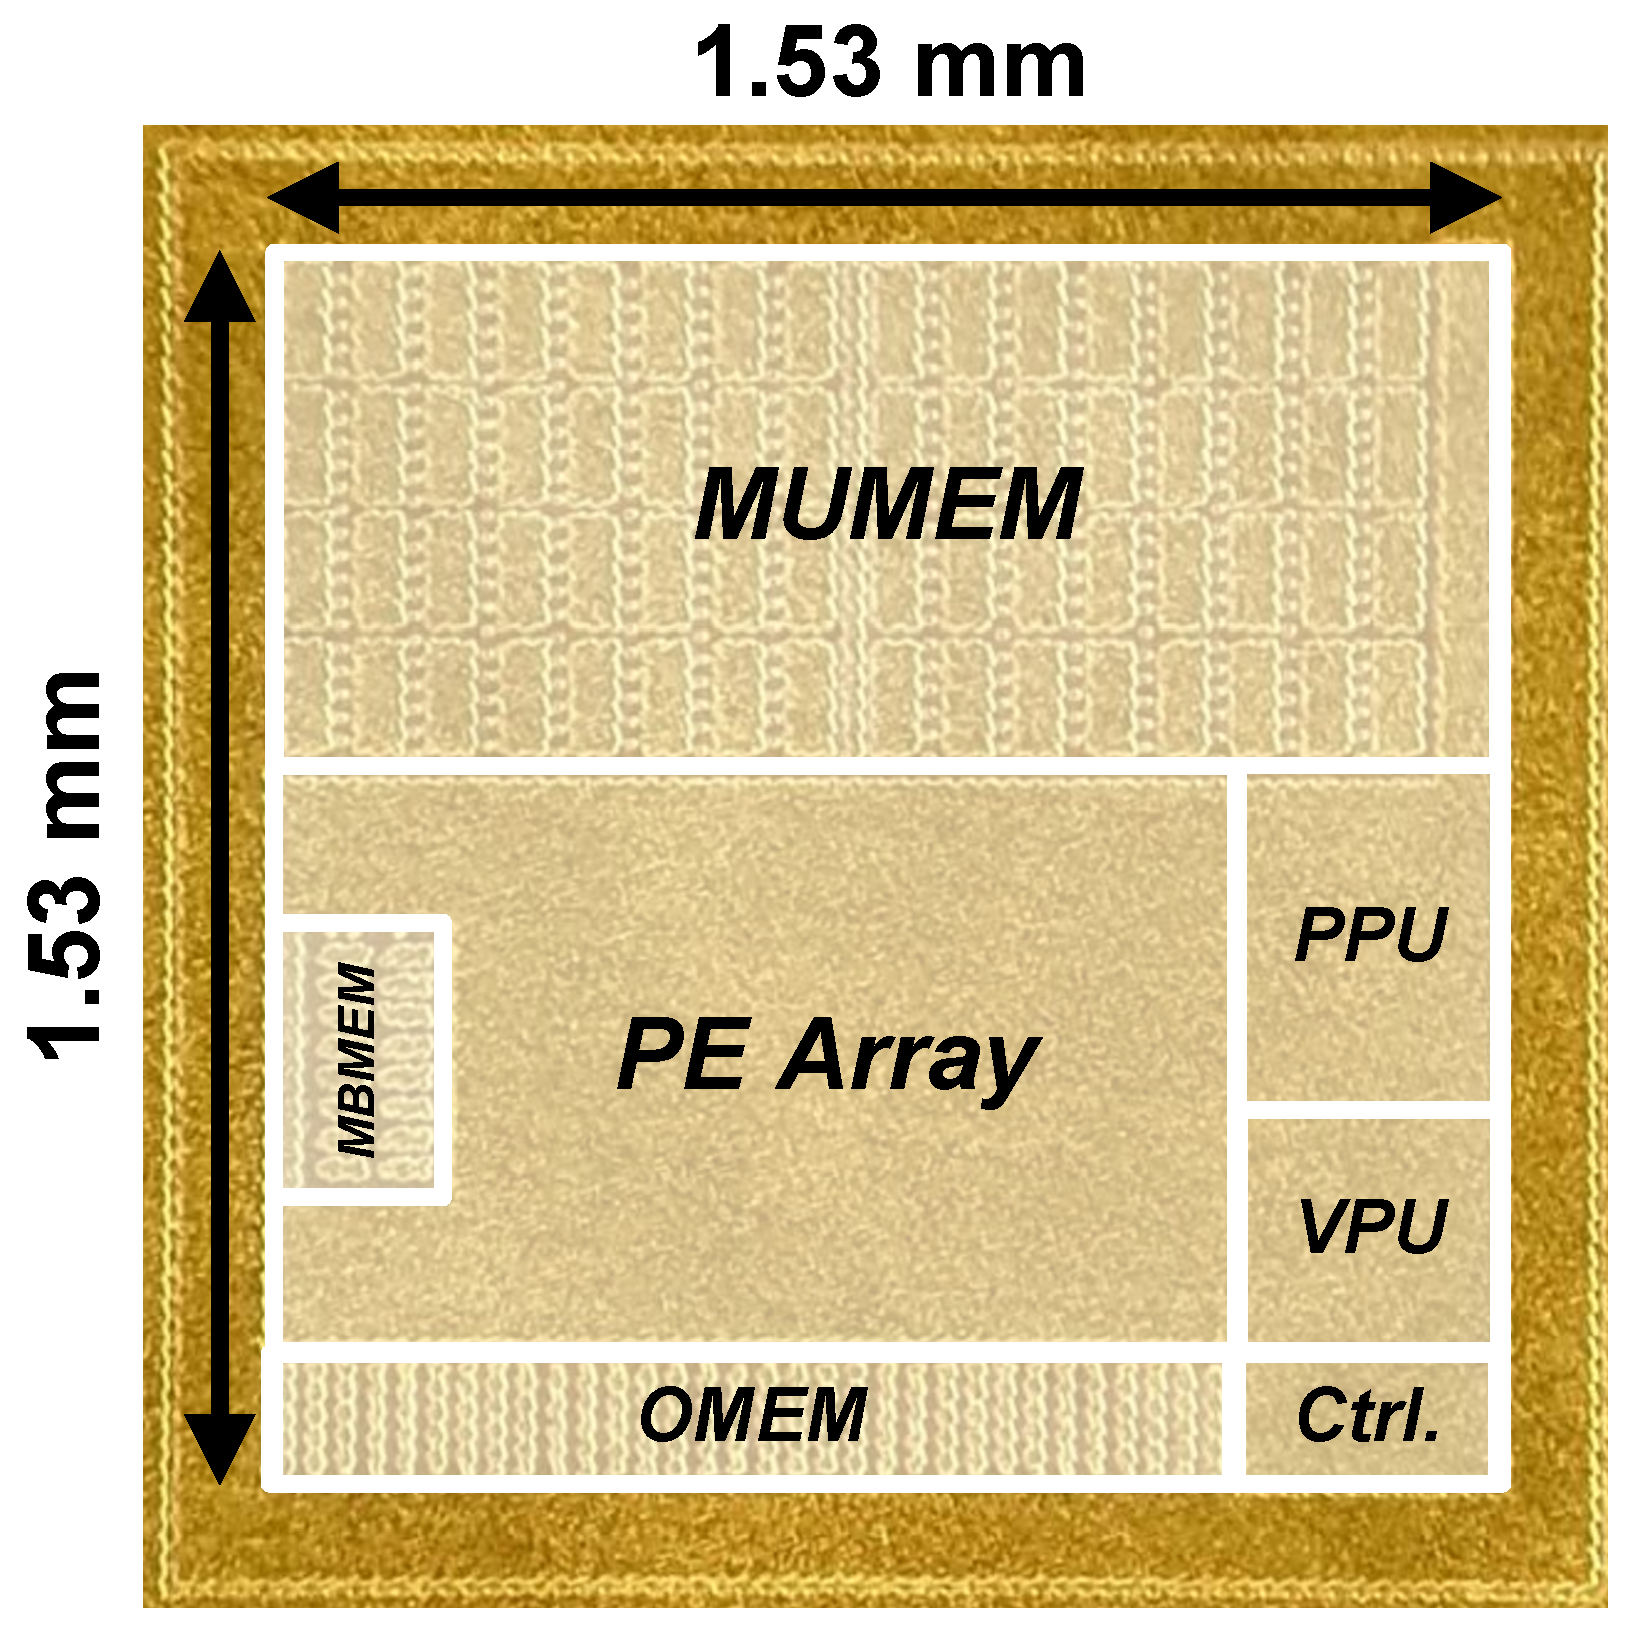
\includegraphics[width=0.6\linewidth]{Figures/Fig_diephoto.pdf}\\
  \caption{Die photograph.}\label{fig:diephoto}
   \end{center}
   % \vspace{-0.7cm}
   \vspace{0.2cm}
\end{figure}

\begin{figure}[!t]
   \begin{center}
  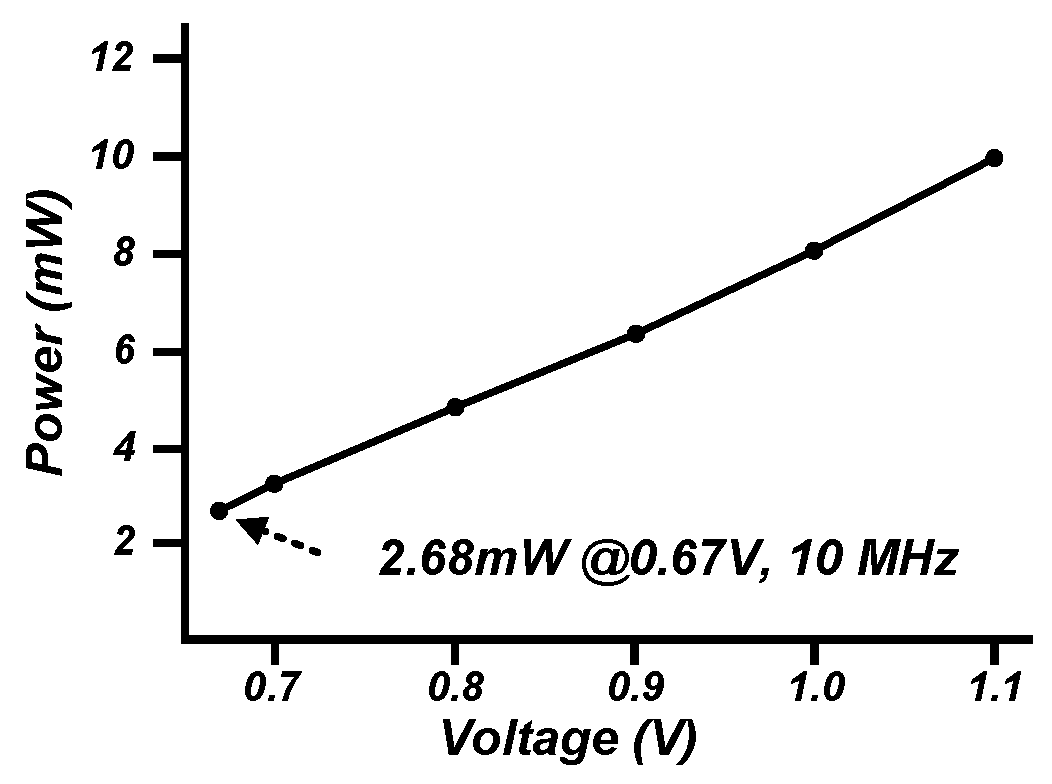
\includegraphics[width=0.7\linewidth]{Figures/Fig_power_meas.pdf}\\
  \caption{Measured power consumption.}\label{fig:power}
   \end{center}
   \vspace{-0.5cm}
\end{figure}



The proposed DRL processor was fabricated in a 28-nm CMOS process, and Fig. \ref{fig:diephoto} shows a die photograph. The design occupies 1.53$\times$1.53 $\text{mm}^2$ area with 592-kB on-chip SRAM. The processor operates at a clock frequency of 10 MHz, meeting the real-time control requirements of the navigation task. Fig. \ref{fig:power} displays the measured power consumption. The processor consumes 2.68 mW during concurrent inference and training at 10 MHz, 0.68 V. Fig. \ref{fig:area_breakdown} shows the area breakdown of the processor. The arithmetic intensity of the hardware is calculated using the reported I/O bandwith and peak performance, excluding other hardware optimization techniques but assuming all feature maps and parameters are loaded at least once. The arithmetic intensity of the model is calculated using the total operations and external memory access required by the model. We also take into account each design’s reported EMA reduction ratio.

\begin{table*}[t]
\centering
\caption{Comparison With State-of-the-Art DRL Processors}
\label{tab:comparison}
\renewcommand{\arraystretch}{2}
\begin{tabular}{|c|c|c|c|c|c|}
\hline
 & \textbf{This Work} & \textbf{ISSCC'19~\cite{ISSCC19}} &
   \textbf{VLSI'21~\cite{VLSI21}} & \textbf{TCAS-II'24~\cite{TCASII24}} &
   \textbf{CICC'25~\cite{CICC25}} \\
\hline
% Verified on Real Robot                       & O &  & X &  &  \\ \hline
% Support for Distributional RL                & O (D4PG) &  & X & X &  \\ \hline
Verified on Real Robot
  & O
  & \multicolumn{4}{c|}{X} \\ \hline

Support for DistRL
  & O
  & \multicolumn{4}{c|}{X} \\ \hline
Technology (nm)                              & 28 & 65 & 28 & 28 & 40 \\ \hline
Area (mm$^{2}$)                              & 2.34 & 16$^a$ & 28$^a$ & 12.96$^a$ & 5.65 \\ \hline
Precision (Weight)                           & Bfloat16 & FXP4/8/16 & Bfloat16 & BFP12/16 & BFP8 \\ \hline
Precision (Activation)                       & Bfloat16 & Bfloat16  & Bfloat16 & BFP12/16 & BFP8 \\ \hline
SRAM (kB)                                    & 592 & 448 & 1552 & 2594 & 108 \\ \hline
EMA Reduction                                & 84.1\% & 41.0\%$^b$ & 51.5\%$^c$ & 45.1\%$^c$ & -- \\ \hline
\makecell{Arithmetic Intensity (Hardware)$^d$ \\ {[OP/Byte]}}    & 32.0 & 127.5 & 404.0 & 1025.0 & -- \\ \hline
\makecell{Arithmetic Intensity (Model)$^e$ \\ {[OP/Byte]}}      & 32.5 & 441.0$^b$ & 108.6$^c$ & 90.8$^c$ & -- \\ \hline
Intensity Ratio                              & 1.02 & 3.46 & 0.27 & 0.09 & -- \\ \hline
\makecell{Processor Utilization \\ for Sparse Training$^f$} & 100\%$^g$ & 12.51\%$^b$ & 12.61\%$^c$ & 12.61\%$^c$ & -- \\ \hline
Voltage (V)                                  & 0.67–1.1 & 0.67–1.1 & 0.68–1.1 & 0.9 & 0.64–1.1 \\ \hline
Power (mW)                                   & \makecell{2.68 \\ (10 MHz, 0.67 V)} &
                                               \makecell{2.4  \\ (10 MHz, 0.67 V)} &
                                               \makecell{6.7  \\ (5 MHz, 0.68 V)}  &
                                               \makecell{176.7 \\ (200 MHz, 0.9 V)} &
                                               \makecell{25.1 \\ (50 MHz, 0.64 V)} \\ \hline
\makecell{Peak Area Efficiency$^h$ \\ (GFLOPS/mm$^2$)}  & 2.19 &
                                                      3.44 &
                                                      2.37 &
                                                      6.33 &
                                                      3.70 \\ \hline
\makecell{Normalized Area Efficiency \\ during DRL Training $^h$ \\ (GFLOPS/mm$^2$)}  & 2.19 &
                                                                                      3.39$^b$ &
                                                                                      0.78$^c$ &
                                                                                      -- &
                                                                                      --\\ \hline



\multicolumn{6}{l}{%
  \begin{minipage}{0.9\linewidth} % 셀 너비에 맞는 minipage 생성
    \vspace{5pt} % 위쪽 여백 살짝 추가 (선택사항)
    \footnotesize
    * All results assume 0\% weight sparsity and no speculation.\\
    $^{a}$Die area.\quad
    $^{b}$Actor–Critic, Hill Climbing, batch 2048.\quad
    $^{c}$TD3, MuJoCo HalfCheetah, batch 256. \\
    $^d$ Calculated using the reported I/O bandwidth and peak performance.\quad
    $^e$ Reported EMA reductions considered. \\
    $^{f}$$\,{(T+N)} \over {N(T+1)}$, $T = {\text{\# Training operations} \over {\text{\# Inference operations}}}$, $N=8$.\quad
    $^{g}$Batch 512. \quad
    $^{h}$Normalized with respect to process and frequency.
  \end{minipage}%
}
 

\vspace{-0.2cm}

\end{tabular}
\end{table*}


Table \ref{tab:comparison} compares our design with state-of-the-art DRL processors. The proposed processor is the only design validated on a real robot and supporting DistRL. Compared to prior designs, the design achieves the largest EMA reduction of 84.1\% and the most balanced arithmetic intensity, with a ratio of 1.02. Furthermore, while previous designs exhibit only 12–13\% utilization under sparse training, the proposed processor can achieve full (100\%) utilization in the same scenario. It should be noted that, despite these advantages, our design is limited to fixed BF16 precision. This design decision was partially based on the experimental results in Fig. \ref{fig:precision_comparison}, which show even FP16 training failed to converge in the target task. Therefore, we considered BF16 to be the minimum viable precision for our design. Contrarily, several recent accelerators support mixed/flexible precision, enabling accuracy-performance trade-offs \cite{ISSCC19} or layer-wise precision selection \cite{TCASII24}. While our design approach with a single precision allows for a simple datapath, our design cannot exploit the benefits of low-precision computing such as energy and throughput gains especially in more error-tolerant models or layers.

\begin{figure}[!t]
   \begin{center}
  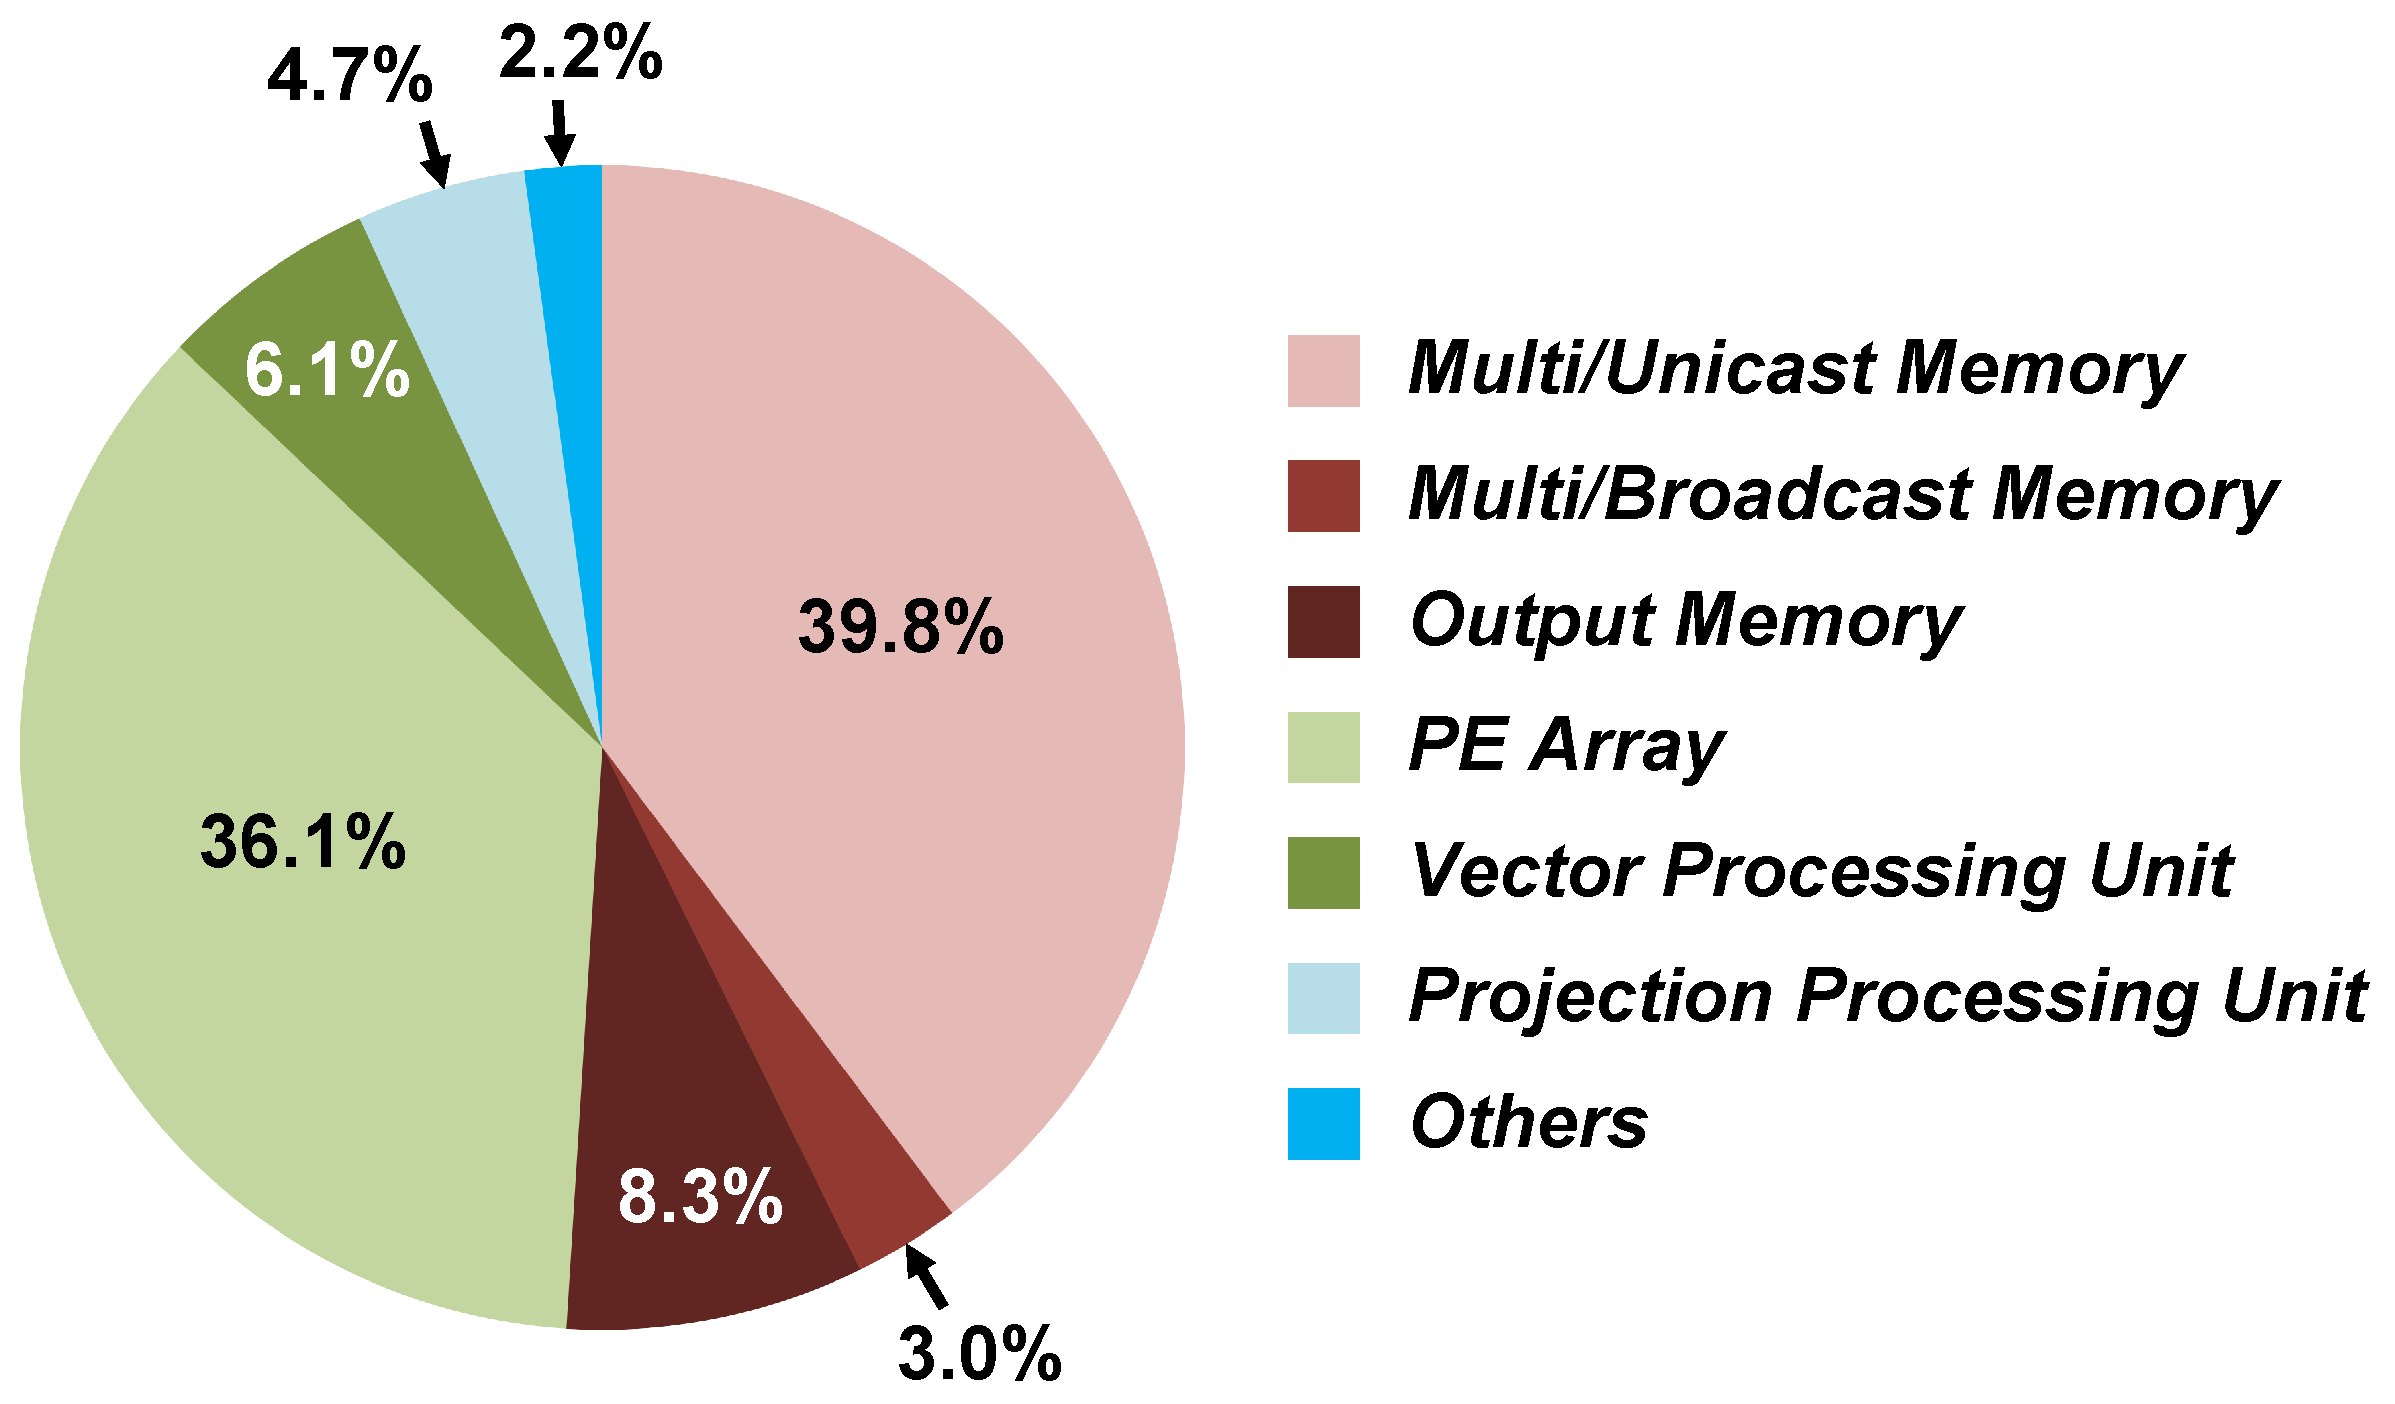
\includegraphics[width=0.9\linewidth]{Figures/Fig_area_breakdown_v2.pdf}\\
  \caption{Area breakdown.}\label{fig:area_breakdown}
   \end{center}
   \vspace{-0.5cm}
\end{figure}

\begin{figure}[!t]
   \begin{center}
   % \captionsetup{skip=-5pt}
  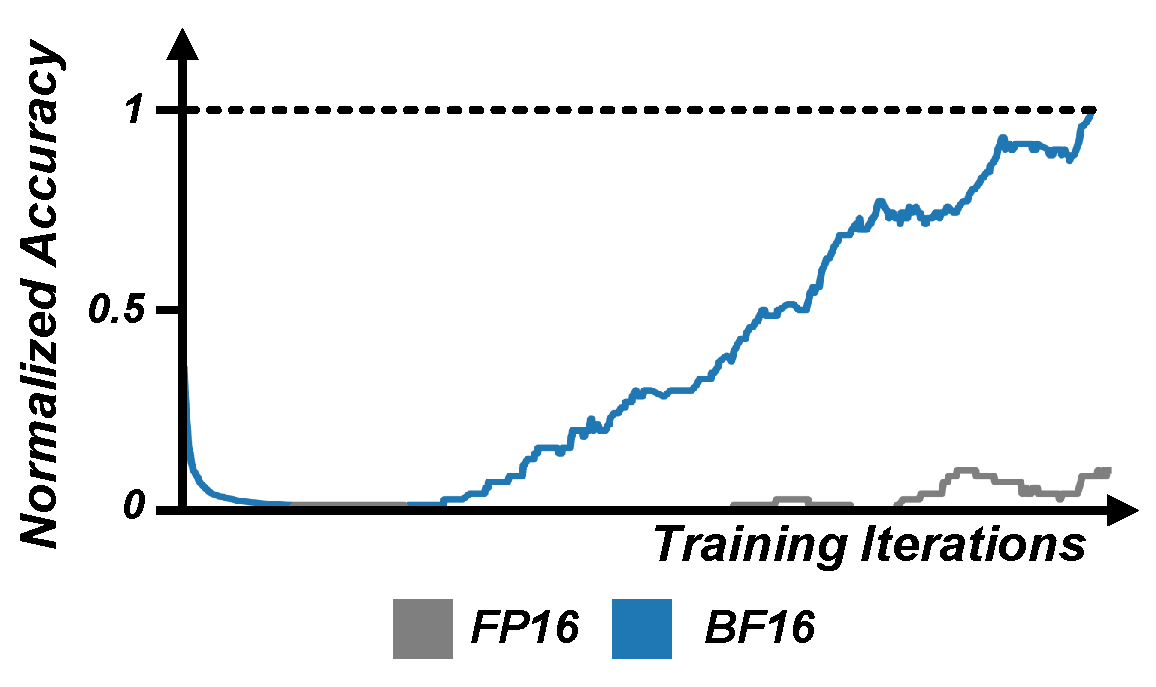
\includegraphics[width=0.83\linewidth]{Figures/Fig_fp16_vs_bf16_v2_cropped.pdf}\\
  \caption{Training performance comparisons between FP16 and BF16.}\label{fig:precision_comparison}
   \end{center}
   \vspace{-0.5cm}
\end{figure}

Unlike simulator-based benchmarks employed in \cite{ISSCC19, VLSI21, TCASII24, CICC25}, our real-time robot navigation workload must remain synchronized with 10 Hz LiDAR sensing and action updates (100 ms period). Under online training, this fixed period and the selected inference-to-training ratio the amount of required computation per unit time, and hence pushing peak throughput beyond it yields diminishing returns. We therefore select a design point that matches the arithmetic intensity between workload and hardware.

Table \ref{tab:comparison} shows that the design in \cite{VLSI21} achieves a peak area efficiency of 2.37 GFLOPS/mm$^2$, but it drops to only 0.78 GFLOPS/mm$^2$ and 1.61 GFLOPS/mm$^2$ during training in HalfCheetah-v2 and Humanoid-v2 environments, respectively, indicating the under-utilization of compute capability. On the other hand, the design in \cite{ISSCC19} reports peak area efficiency of 3.44 GFLOPS/mm$^2$ using lower weight precisions (FXP4/8/16). The compute-bounded operating point with arithmetic intensity ratio of 3.46 yields only a small area efficiency degradation during actual training, but external I/O bandwidth remains significantly under-utilized. In contrast, our arithmetic-intensity-matched design delivers identical peak and training area efficiencies of 2.19 GFLOPS/mm$^2$, confirming that our design is well-optimized for the target navigation workload.

\subsection{Navigation Performance in Simulation}

\begin{figure}[!t]
   \begin{center}
  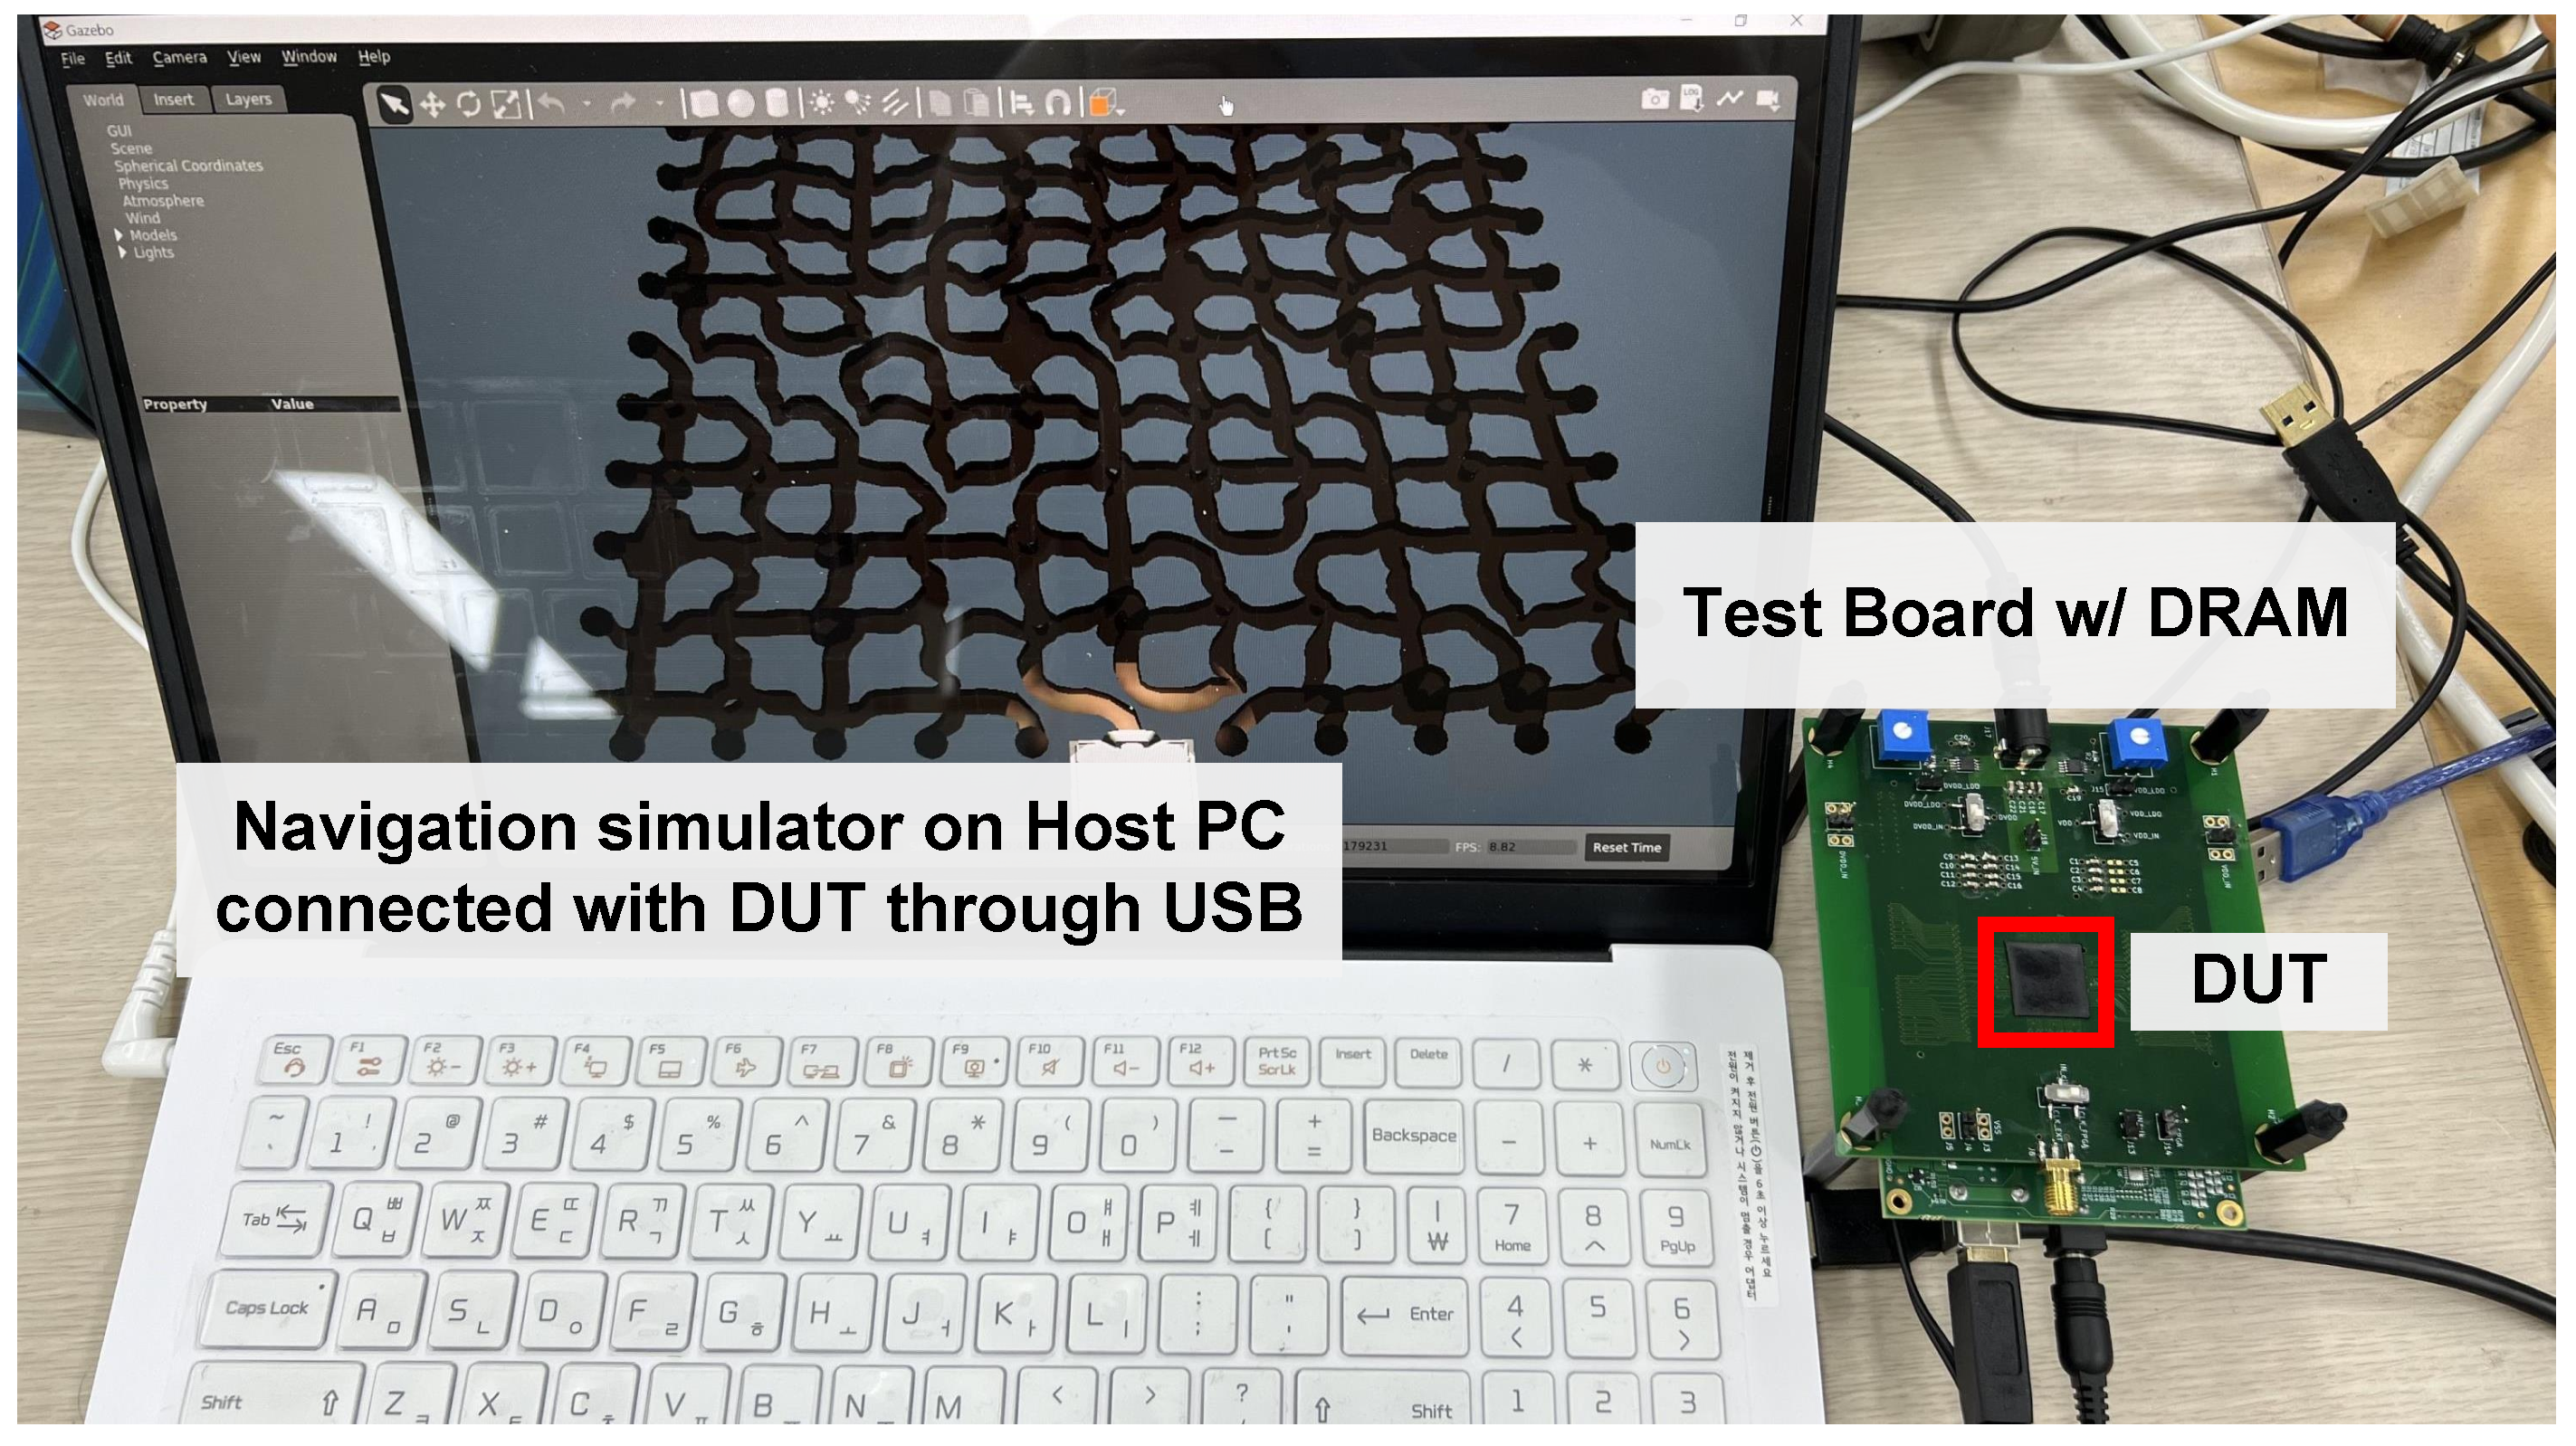
\includegraphics[width=0.9\linewidth]{Figures/Fig_simulation_environment.pdf}\\
  \caption{Evaluation setup for navigation simulation.}\label{fig:simulation_environment}
   \end{center}
   \vspace{-0.8cm}
\end{figure}

Fig. \ref{fig:simulation_environment} shows the evaluation setup for navigation simulation. The FPGA board interfaces the processor with the host PC, which runs the navigation simulator and emulates the real sensor by generating simulated sensor data. This data is transferred to the processor via FPGA, where the processor performs network training and generates actions based on the received sensor data. The actions are sent back to the simulator through FPGA, prompting the simulator to advance one step and generate new sensor data along with the corresponding reward. This closed-loop process is repeated for the entire training duration. In addition to serving as an interface, FPGA is equipped with on-board DRAM and functions as a DRAM controller, enabling data transfer between the processor and external memory.


\begin{figure}[!t]
\centering

\subfloat[]{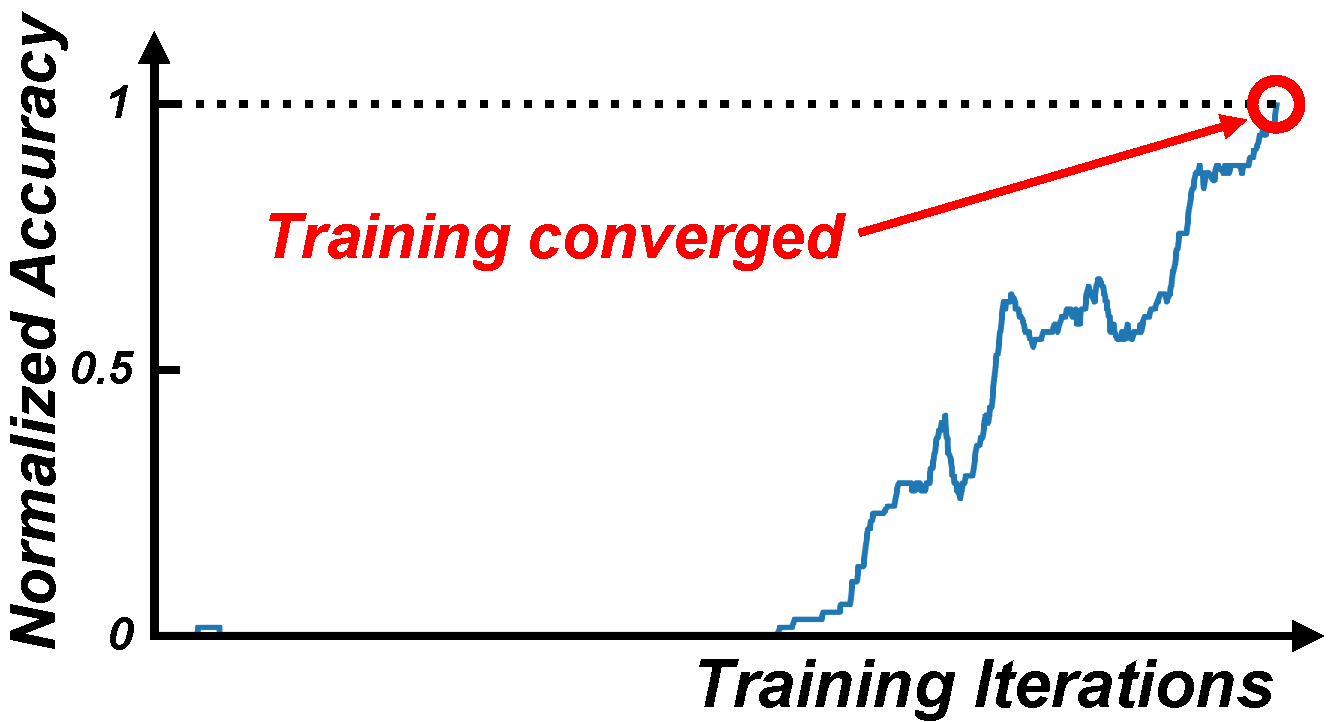
\includegraphics[width=0.5\linewidth]{Figures/Fig_sim_result_cave_v2.pdf}\label{fig:sim_cave}}
\subfloat[]{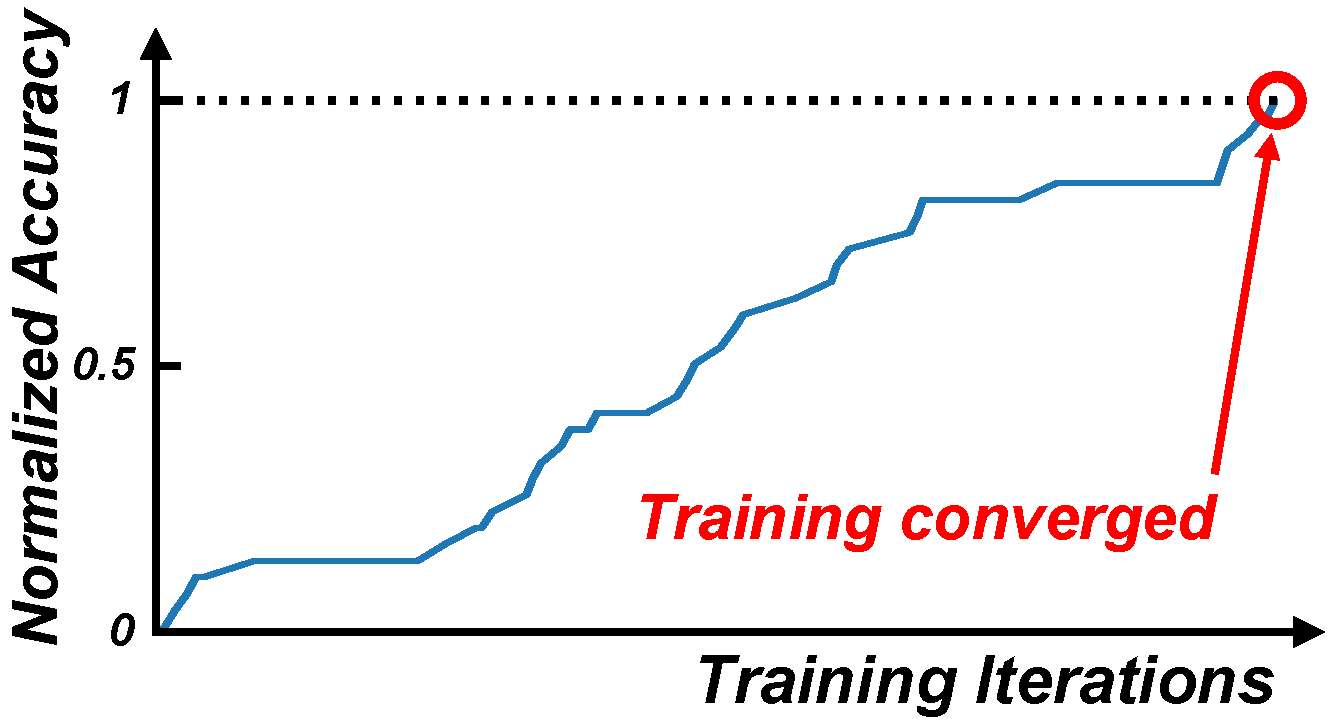
\includegraphics[width=0.5\linewidth]{Figures/Fig_sim_result_indoor_v2.pdf}\label{fig:sim_indoor}}

\subfloat[]{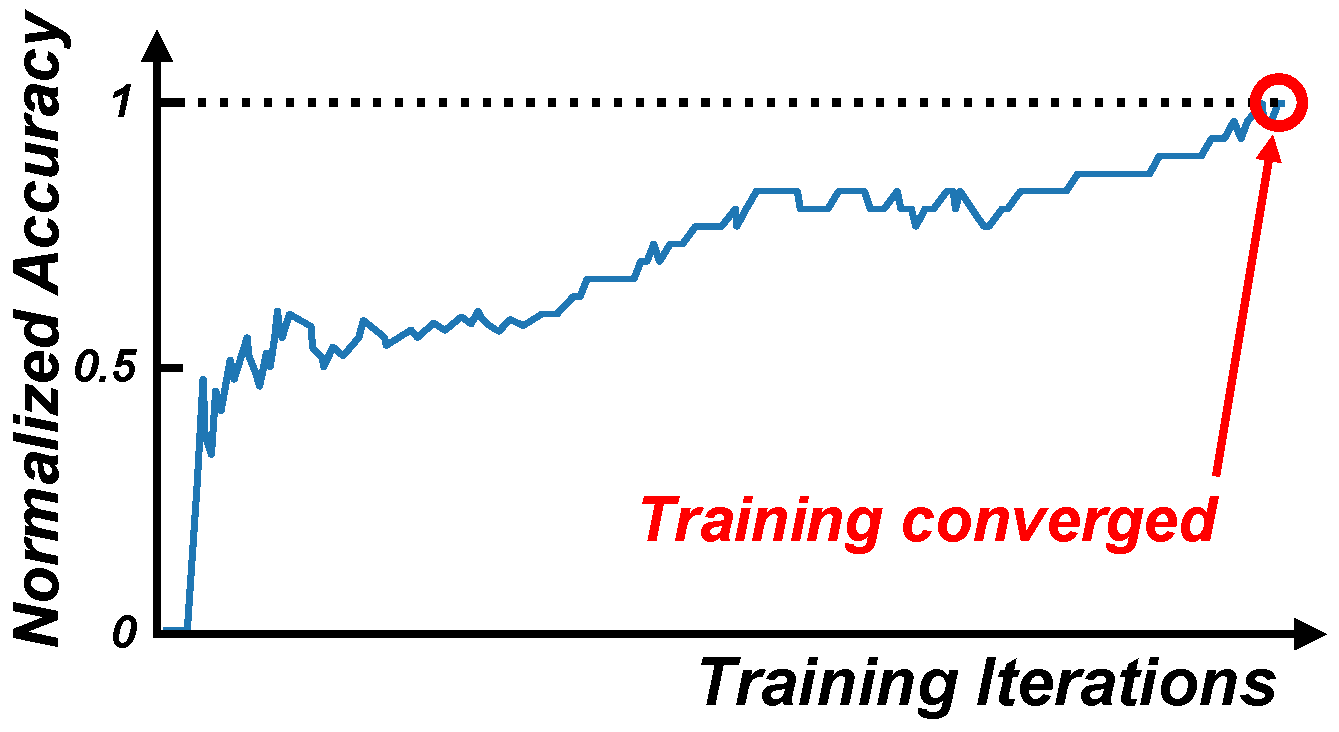
\includegraphics[width=0.5\linewidth]{Figures/Fig_sim_result_garage_v2.pdf}\label{fig:sim_garage}}
\subfloat[]{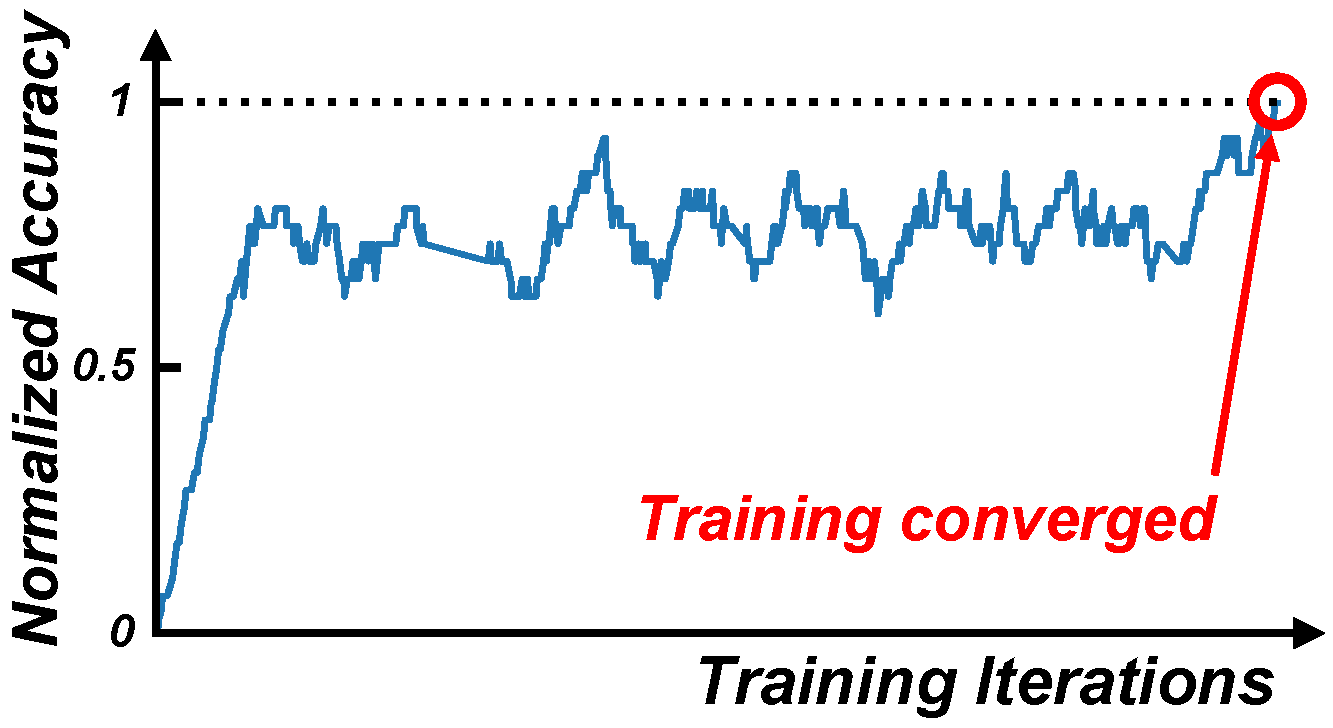
\includegraphics[width=0.5\linewidth]{Figures/Fig_sim_result_forest_v2.pdf}\label{fig:sim_forest}}

\caption{Learning curves in various simulation environments: (a) Cave, (b) Indoor, (c) Garage, and (d) Forest. }\label{fig:simulation_results}
\vspace{-0.5cm}
\end{figure}

Fig. \ref{fig:simulation_results} shows the learning curves obtained using the navigation simulator in various environments, including Cave \cite{env_cave} as well as Indoor, Garage, and Forest from \cite{env_others}. The results demonstrate that the proposed system achieves stable convergence in all tested environments, confirming its robustness and generalization capability across diverse navigation scenarios.

\subsection{Navigation Performance in Real-World Experiments}

\begin{figure}[!t]
   \begin{center}
  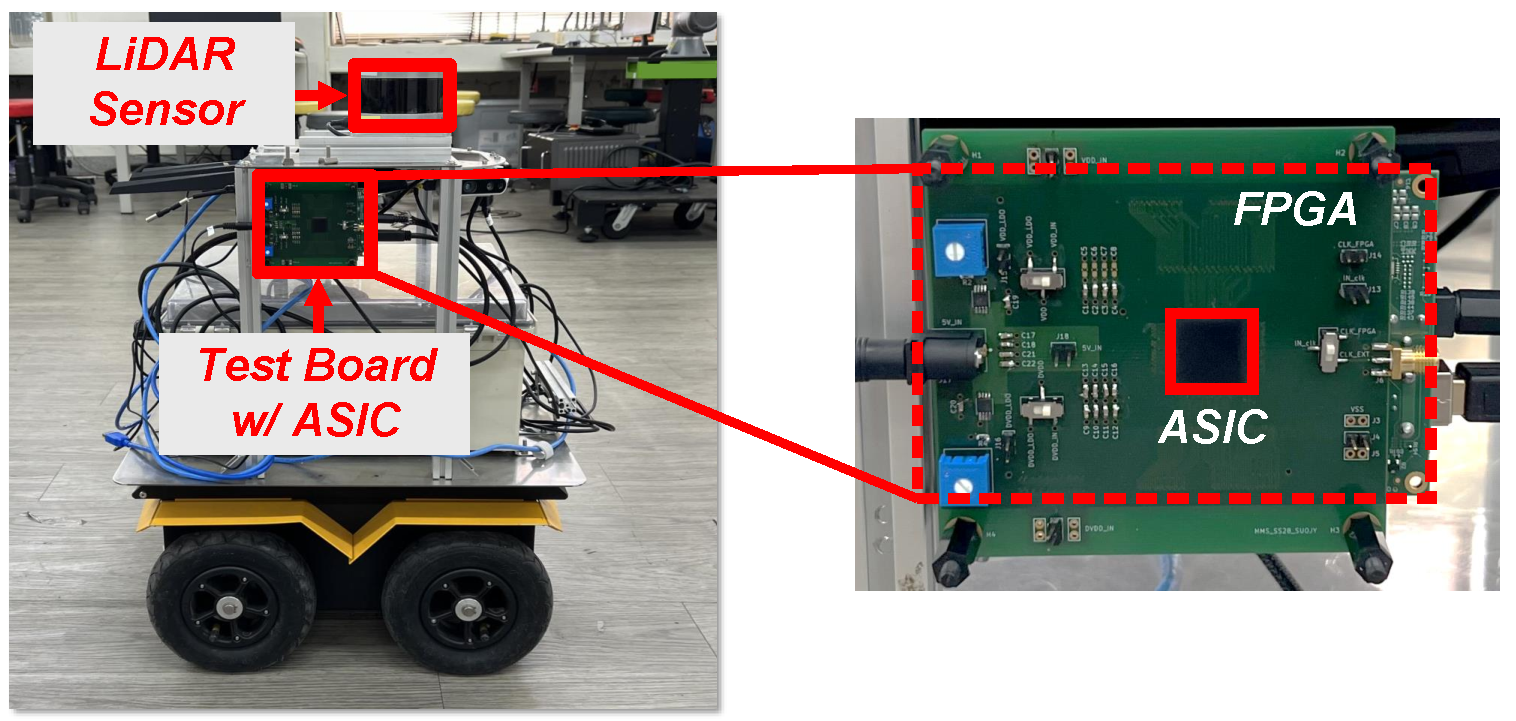
\includegraphics[width=1\linewidth]{Figures/Fig_robot_setup.pdf}\\
  \caption{Real-world verification platform.}\label{fig:robot_setup}
   \end{center}
   \vspace{-0.5cm}
\end{figure}

\begin{figure}[!t]
\centering

\subfloat[]{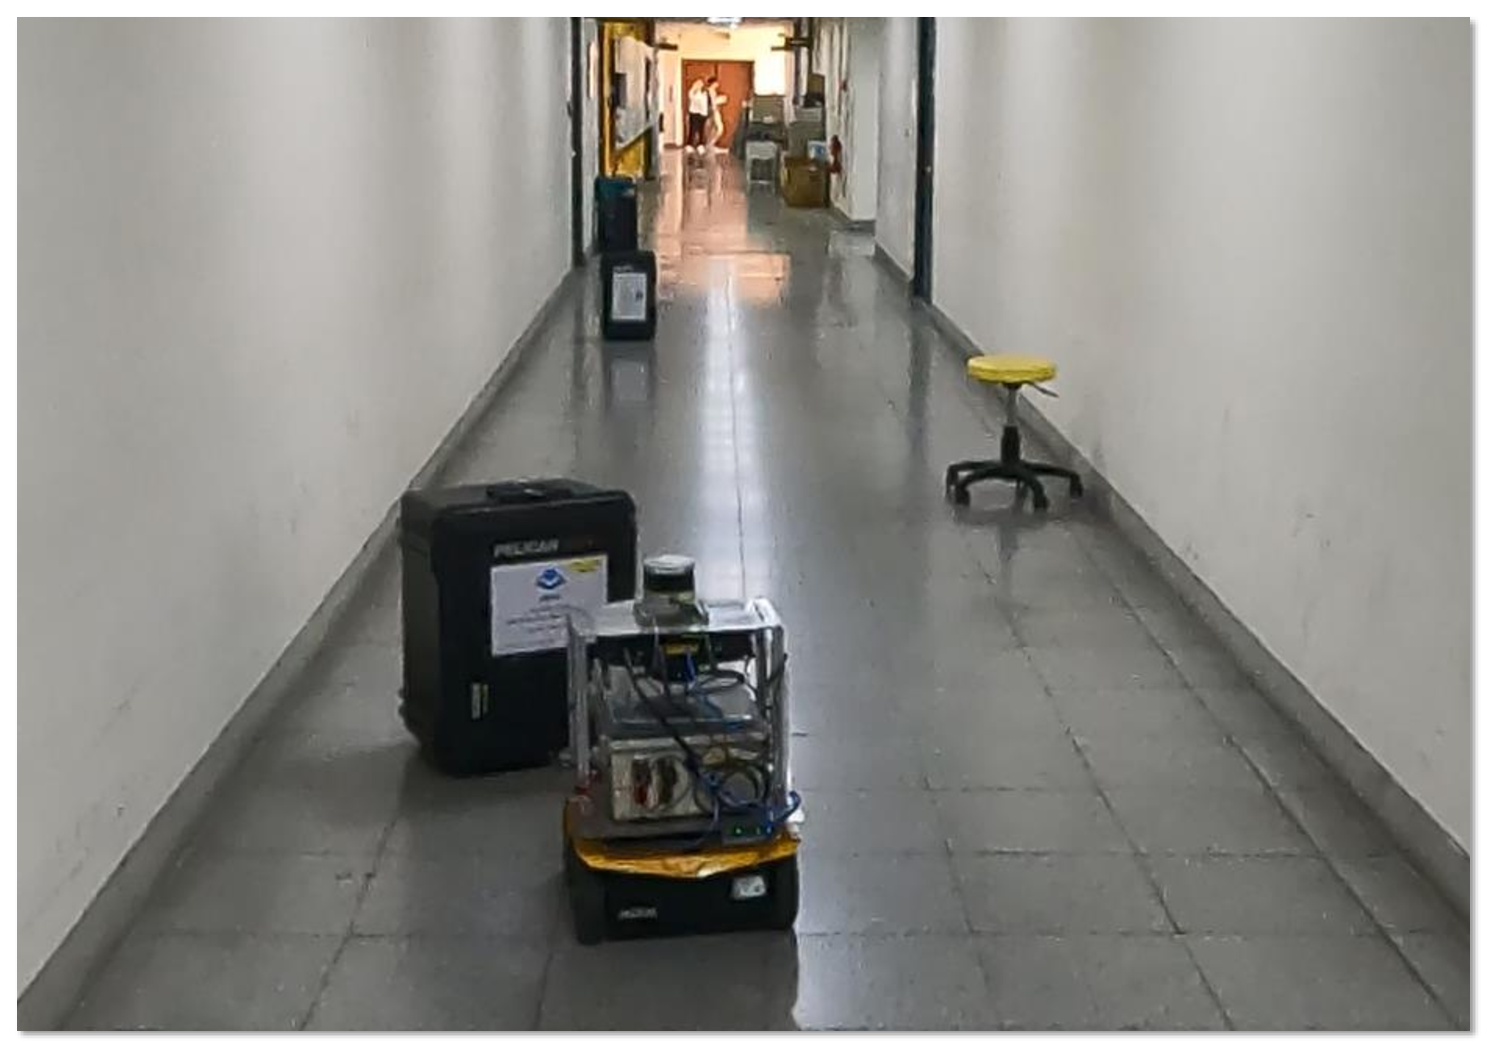
\includegraphics[width=1\linewidth]{Figures/Fig_env.pdf}\label{fig:real_env}}

\subfloat[]{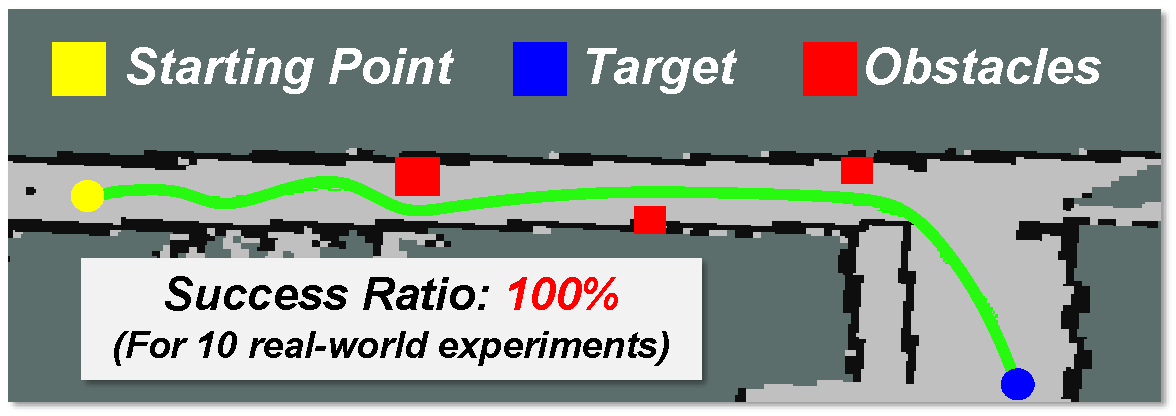
\includegraphics[width=1\linewidth]{Figures/Fig_trajectory.pdf}\label{fig:trajectory}}


\caption{(a) Indoor verification environment and (b) measured trajectory. }\label{fig:real_results}
\vspace{-0.5cm}
\end{figure}

To validate the functionality of the proposed processor beyond simulation, real-world experiments were conducted using an actual robot. A Jackal UGV (Clearpath Robotics) \cite{jackal} with sensor input period and control rate of both 10Hz was used for the experiment. The proposed processor was integrated into the robotic platform via an FPGA interface, as shown in Fig. \ref{fig:robot_setup}. Fig. \ref{fig:real_results}\subref{fig:real_env} presents the indoor environment used for the real-world verification, located at National Yang Ming Chiao Tung University (NYCU) in Taiwan. The test environment consisted of narrow corridors with multiple obstacles placed along the robot's path, requiring the robot to navigate from a start position to an unseen target location without collision. The trajectory is approximately 30 m, and the robot requires about 1 minute to reach the goal. In real-world experiments, the robot operated with weights pre-trained in the Indoor environment from \cite{env_others} and no additional online training was performed. Between 25,000 and 30,000 iterations were required for training convergence in the Indoor environment.

In real-world experiments, we introduced obstacles that were absent during pre-training. Even in this previously unseen configuration, the robot reached the target wighout collisions. However, we consistently observed a brief pause before the avoidance maneuver. These results indicate that pre-trained policy can avoid collision for unseen environment, but it shows suboptimal avoidance latency. We therefore expect that online adaptation in the target environment would reduce avoidance latency and yield a well-aligned navigation policy.

Over 10 independent trials, the robot successfully reached the goal in all attempts without any collision, demonstrating stable and robust operation in unseen environment. Fig. \ref{fig:real_results}\subref{fig:trajectory} displays the recorded trajectory. The illustrated map is provided only for the visualization purpose and is not used in the navigation. The robot reached the target position without collision, successfully avoiding obstacles throughout the entire path. These real-world experiments confirm that our design is capable of reliable operation when deployed on an actual robotic system.
 
\section{Conclusion} \label{sec:conclusion}
In this paper, real-time reinforcement learning processor for mapless autonomous navigation, designed to meet the tight resource and energy constraints of mobile robotic platforms, is proposed. The proposed processor features a unified actor-critic network architecture that enables parameter sharing between the actor and critic branches, together with feature map caching to eliminate redundant computation, resulting in a reduction of total parameters, external memory access, and overall operations by 95.6\%, 84.1\%, and 85.4\%, respectively. IoR scheduling allows inference requests to interrupt background training, thereby maintaining full hardware utilization across a wide range of inference-to-training ratios. Adaptive dataflow mapping scheme efficiently supports all of multi-/single-batch feed-forwards, and activation/weight gradient calculations without additional data transposition, achieving high PE array utilization of 71.0\% including external I/O latency. Column-wise zero-skipping categorical projection fetches and processes only non-zero elements in the sparse $\Delta h$ matrix, enabling efficient hardware acceleration for DistRL algorithms. Fabricated in a 28-nm CMOS process, the processor consumes only 2.68 mW at 0.68 V and 10 MHz while meeting the real-time constraints of autonomous navigation. To the best of our knowledge, this is the first DRL processor that provides hardware support for DistRL, and real robot experiments confirm both the effectiveness and practicality of the proposed design.



\section*{Acknowledgement}
The chip fabrication and EDA tool were supported by the IC Design Education Center.

% \bibliographystyle{IEEEtran}
% \bibliography{IEEEabrv,Bibliography}
% \bibliography{Bibliography}
% \printbibliography

\ifCLASSOPTIONcaptionsoff
  \newpage
\fi

\bibliographystyle{IEEEtran} %TODO: insert biography
\bibliography{IEEEabrv,Bibliography}


\begin{IEEEbiography}
[{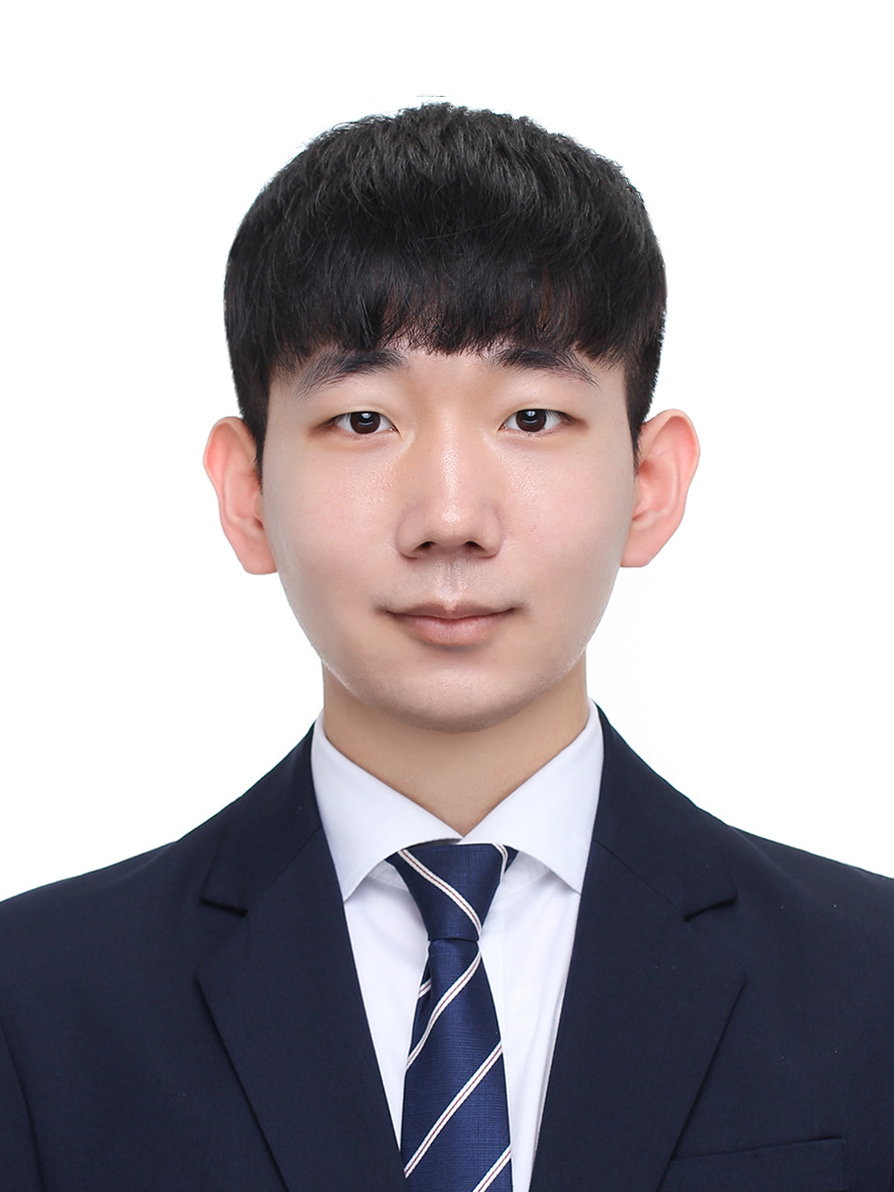
\includegraphics[width=1in,height=1.25in,clip,keepaspectratio]{Photos/JuyoungOh.png}}]{Juyoung Oh}
(Graduate Student Member, IEEE) received the B.S. degree in Electrical and Electronics Engineering from Chung-Ang University, Seoul, South Korea, in 2022. He is currently pursuing a Ph.D. degree at Seoul National University, Seoul, South Korea.
His research interests include hardware/software algorithm co-design and low-power application-specific integrated circuit (ASIC) design for deep learning and robotics applications.
\end{IEEEbiography}

% \vspace{-1.0\baselineskip}

\begin{IEEEbiography}[{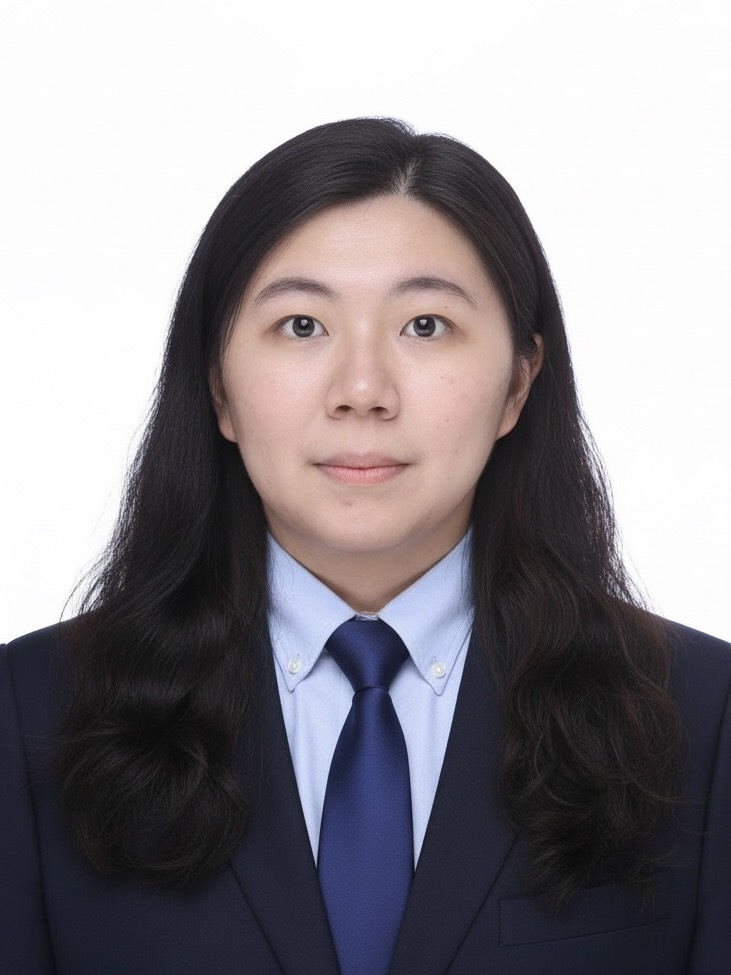
\includegraphics[width=1in,height=1.25in,clip,keepaspectratio]{Photos/Phoebe.jpg}}]{Jie-Xin Liu} received the B.S. degree from the Arete Honors Program at National Yang Ming Chiao Tung University, Hsinchu, Taiwan, in 2023, and the M.S. degree from the Graduate Degree Program of Artificial Intelligence at the same university in 2025. Her research interests include autonomous ground and surface vehicle
navigation, as well as reinforcement learning-based control.
\end{IEEEbiography}

% \vspace{-1.0\baselineskip}

\begin{IEEEbiography}[{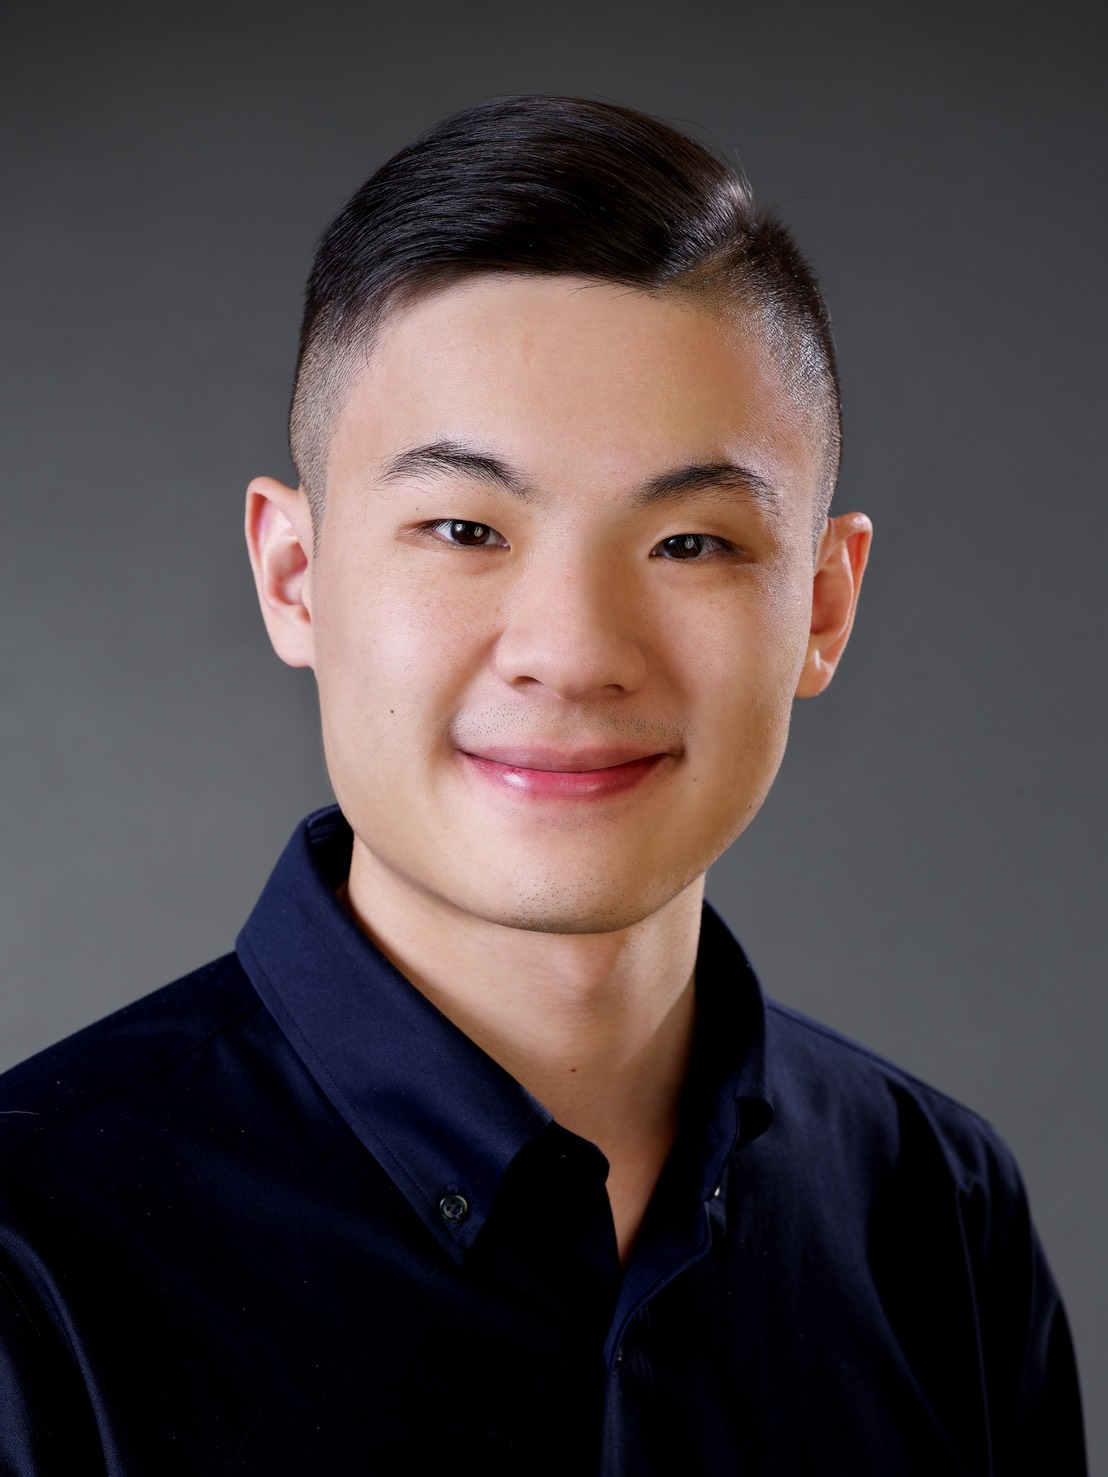
\includegraphics[width=1in,height=1.25in,clip,keepaspectratio]{Photos/Mike.jpg}}]{Yi-Chen Teng} received the B.S. degree in Electrical Engineering from National Central University, Taoyuan, Taiwan, in 2022, and the M.S. degree from the Graduate Degree Program of Robotics at National Yang Ming Chiao Tung University, Hsinchu, Taiwan, in 2024. His research interests include autonomous ground and surface vehicle
navigation, and reinforcement learning-based control.
\end{IEEEbiography}

% \vspace{-1.0\baselineskip}

\begin{IEEEbiography}[{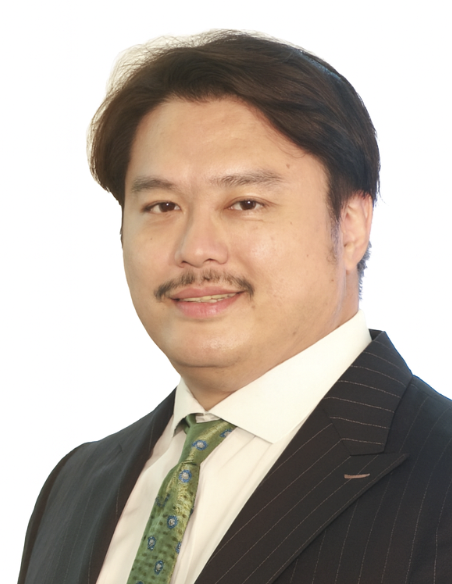
\includegraphics[width=1in,height=1.25in,clip,keepaspectratio]{Photos/Hsueh-Cheng_Wang.png}}]{Hsueh-Cheng Wang}
(Member, IEEE) is an associate professor in the Department of Electrical and Computer Engineering, National Yang Ming Chiao Tung University, Taiwan. He was a postdoctoral associate in the Marine Robotics Group (MRG) in the Computer Science and Artificial Intelligence Laboratory (CSAIL), MIT from 2013 to 2016. Dr. Wang received Ph.D. from the Department of Computer Science, UMass Boston. Dr. Wang's research team focuses on Learning-based Robotic Control, with a strong emphasis on practical applications. Dr. Wang’s team actively participated in international competitions to validate their algorithms in real-world scenarios. Their areas of application span across disaster relief, defense, and smart healthcare, among others.
\end{IEEEbiography}

% \vspace{-10\baselineskip}

\begin{IEEEbiography}[{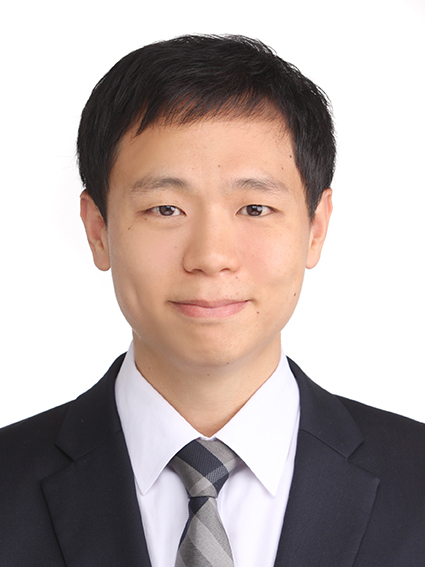
\includegraphics[width=1in,height=1.25in,clip,keepaspectratio]{Photos/dongsuk_jeon.jpg}}]{Dongsuk Jeon}
(Member, IEEE) received the B.S. degree in electrical engineering from Seoul National University, Seoul, South Korea, in 2009, and the Ph.D. degree in electrical engineering from the University of Michigan, Ann Arbor, MI, USA, in 2014. From 2014 to 2015, he was a Postdoctoral Associate with Massachusetts Institute of Technology, Cambridge, MA, USA. He is currently a Professor with the Graduate School of Convergence Science and Technology, Seoul National University. His current research interests include hardware-oriented machine learning algorithms, hardware accelerators, and low-power circuits.
Dr. Jeon has served or is currently serving on the Technical Program Committees of the IEEE International Solid-State Circuits Conference (ISSCC), ACM/IEEE Design Automation Conference (DAC), IEEE/ACM Asia and South Pacific Design Automation Conference (ASP-DAC), and IEEE Asian Solid-State Circuits Conference (ASSCC). He was also a Distinguished Lecturer of the IEEE Solid-State Circuits Society in 2023-2024 and is currently serving as an Associate Editor of the IEEE Transactions on Very Large Scale Integration (VLSI) Systems.
\end{IEEEbiography}


\end{document}
